
This chapter presents the results obtained by the optimization algorithm for classical control strategies. An optimized controller design was obtained for each control strategy and its dynamic stiffness, step  and frequency responses were evaluated. 

Each response is shown in a separate figure that contains four curves which comprise initial and optimized design evaluation in two fluid temperatures each. The tests with two temperatures were performed to cover the entire actuator operation range, from -15$^{\circ}$C to 100$^{\circ}$C.

\section{Classic Controllers and Simple Cost Function}

The classic controllers P, PI, PD and PID were optimized. The initial solutions selected as an input to the optimization algorithm are the controller designs proposed by \citeonline{Ballesteros} and are listed in table \ref{table:5_1_InitSolutTable}.

\begin{table}[H]
	\captionof{table}{Initial Solution for Classic Controllers}
	\label{table:5_1_InitSolutTable}
	\centering
	\resizebox{8cm}{!} {
		\begin{tabular}{|l|c|c|c|c|}
			\hline
			Parameter & P & PI 		& PD 	& PID 	\\ \hline
			$K_p$ & $40$  & $40$	& $40$	& $40$	\\ \hline
			$K_i$ & $0.0$ & $1e-6$	& $0.0$ & $1e-6$\\ \hline
			$K_d$ & $0.0$ & $0.0$	& $0.7$ & $0.7$ \\ \hline
	\end{tabular}}
\end{table}

The results presented in this section were obtained using the simple cost function described by Equations \ref{eq:4_4_2_CostEquation} and \ref{eq:4_4_2_PartialCostEquation}.

\subsection{Proportional Controller (P)}

The optimization results for the proportional controller are presented in this section. As shown in table \ref{table:5_1_1_PContExecution}, the execution time of the optimization was 5.6 hours and 15 
iterations were performed until stopping criteria was reached. Also, the proportional gain after optimization was 84.3. This value is in the range evaluated by \citeonline{Ballesteros} and therefore similar behavior as the one observed by the author is expected. 

\begin{table}[H]
	\captionof{table}{P Controller Optimization Execution Results}
	\label{table:5_1_1_PContExecution}
	\centering
	\resizebox{7cm}{!} {
	\begin{tabular}{|l|c|}
		\hline
		Optimized Proportional Gain & 84.3 \\ \hline
		Optimization Execution Time (h) & 5.6 \\ \hline
		Number of Iterations & 15 \\ \hline		
		Number of Obj. Function Evaluations & 32 \\ \hline			
	\end{tabular}}
\end{table}

The  dynamic stiffness response for each design is shown in Figure \ref{fig:5_1_1_P_DynStif}. The dynamic stiffness for high fluid temperature is considerably lower than for low temperature which reinforces the use of high temperature response to calculate the cost function as discussed in section \ref{4-4-1-DynStiffTest}.

An increase in dynamic stiffness is observed below 4Hz but, for frequencies up to 15Hz a decrease occurred. The dynamic stiffness is more critical at 15Hz because for greater frequencies, more stiffness is required to avoid coupling between control surface rotational mode and aircraft aeroelastic modes \cite{Ballesteros}. Thus, because of the dynamic stiffness decrease at 15Hz, the actuation system with the optimized controller has a worse flutter suppression characteristic than with the initial controller. 

\begin{figure}[H]
	\centering
	\centerline{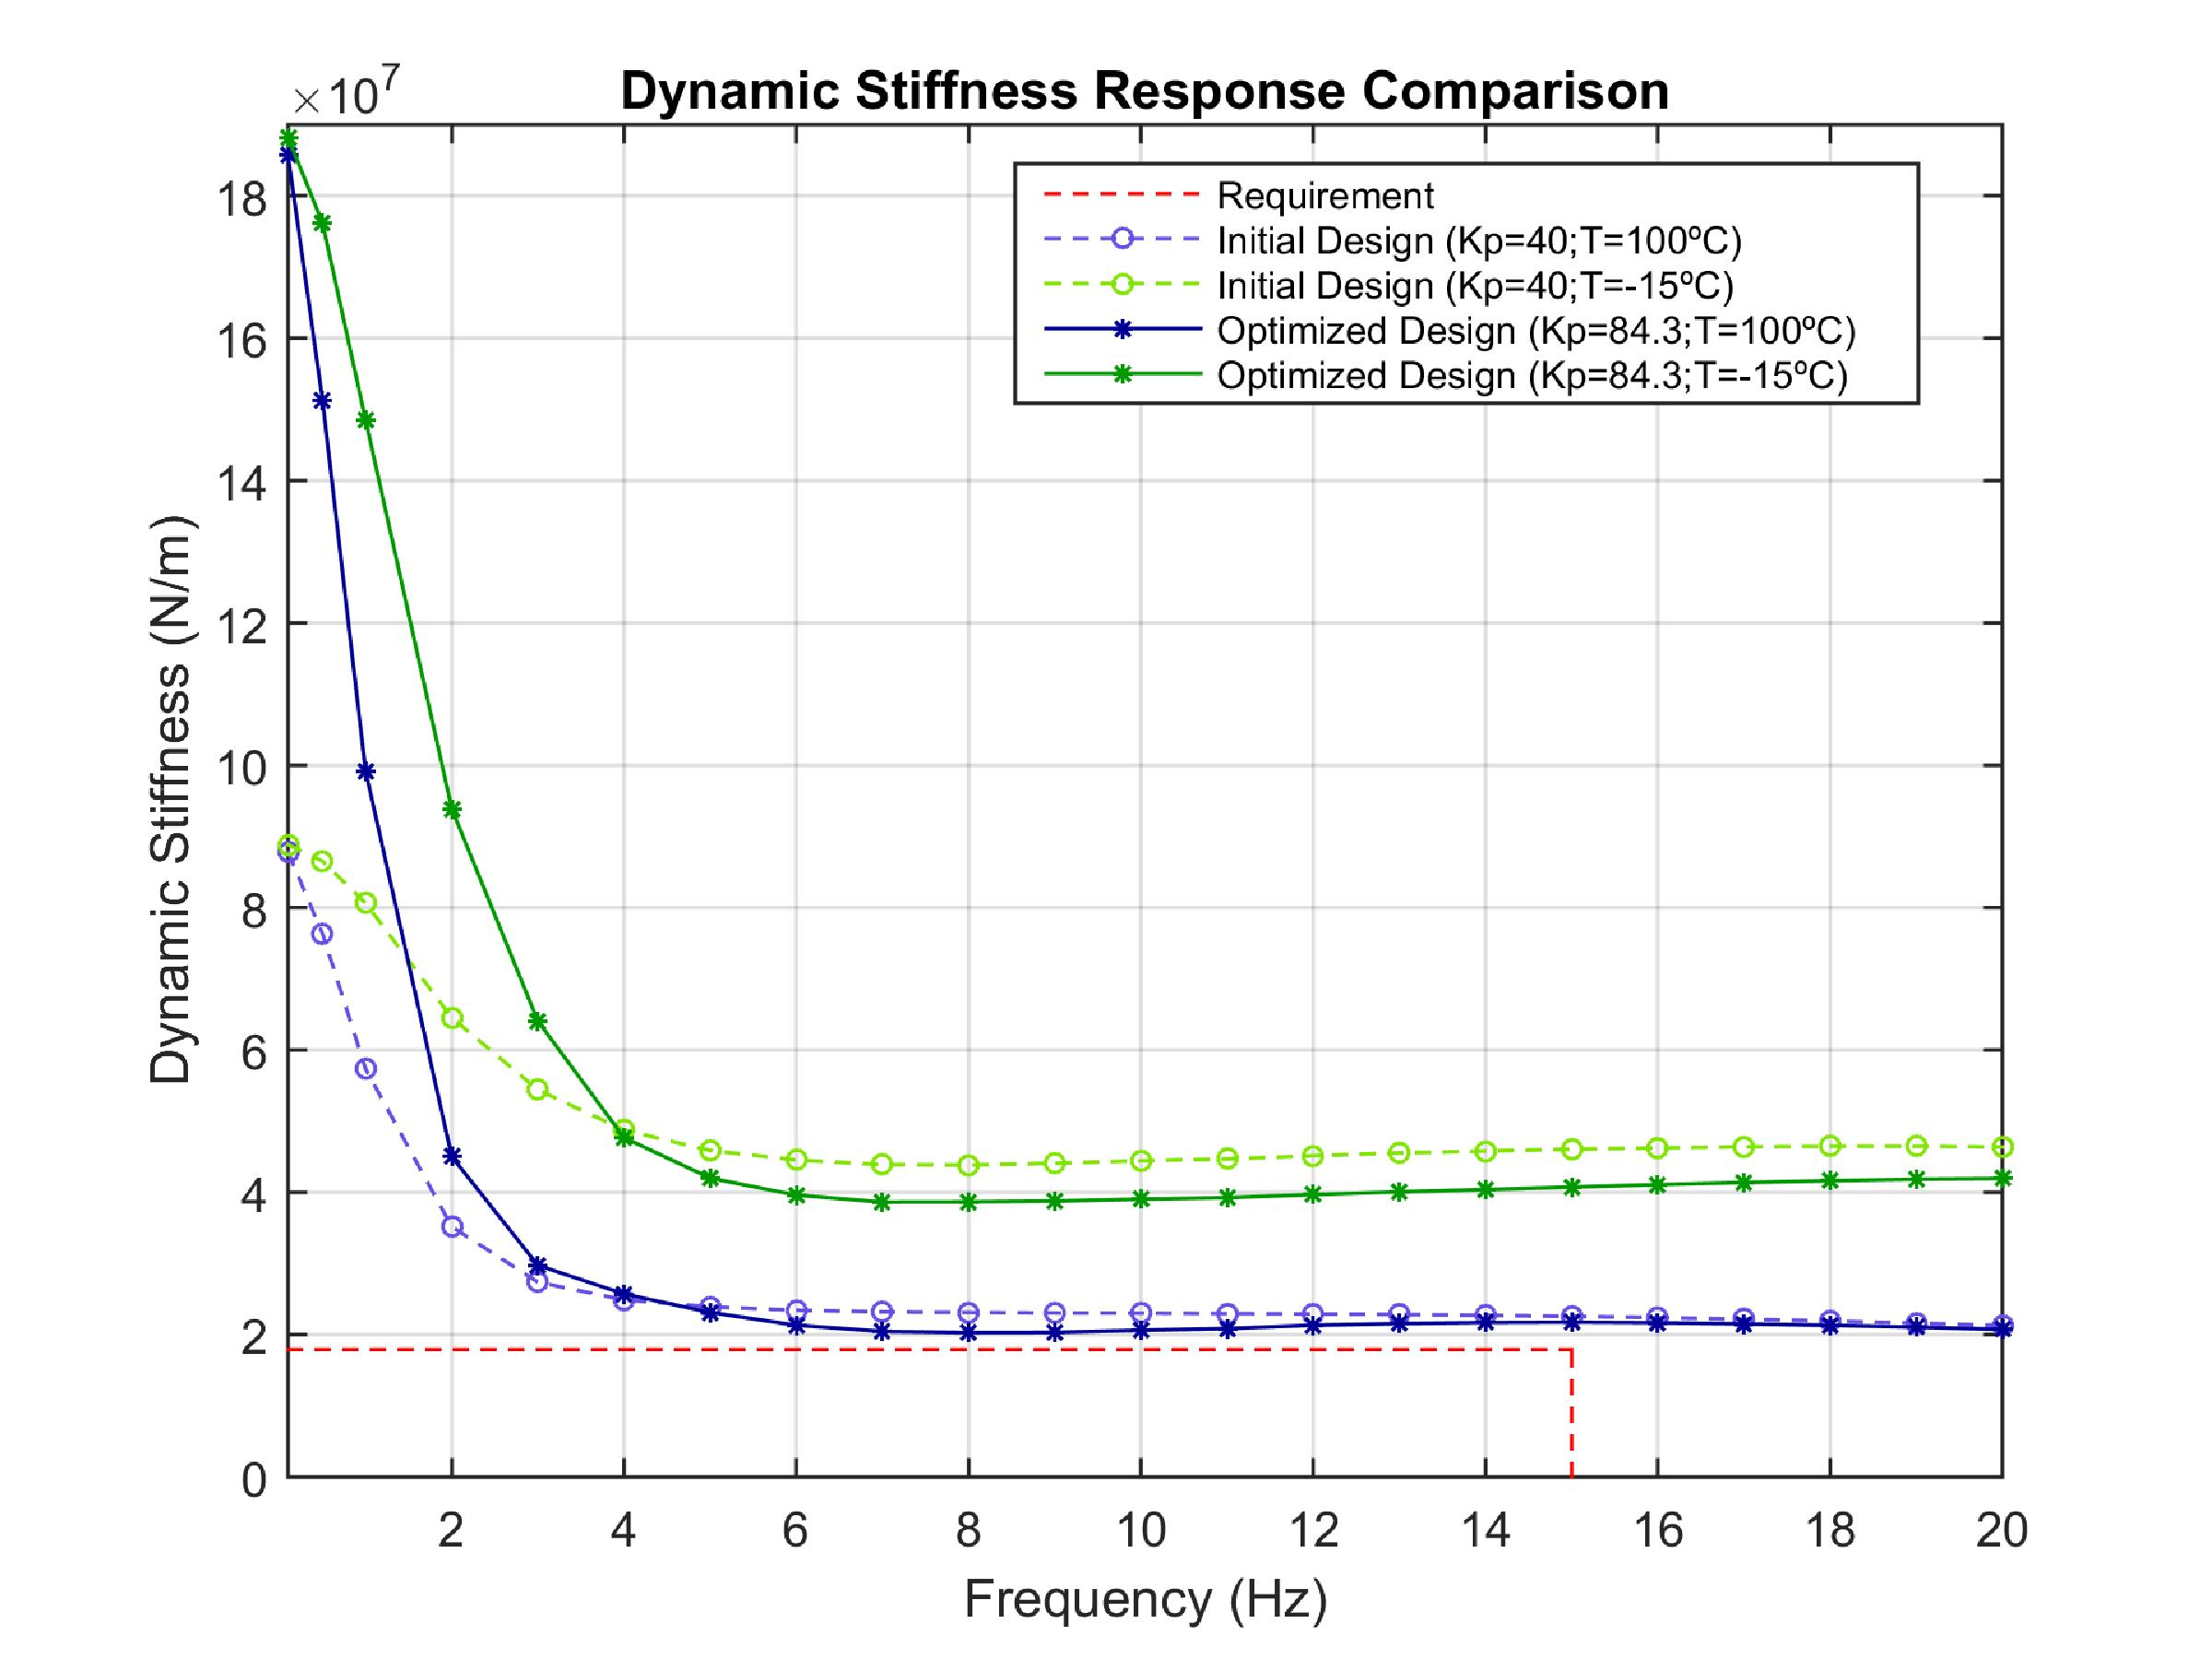
\includegraphics[width=0.9\textwidth]{Figuras/5.OptimizationResults/5-1-1-P-DynamicStiffnessComparison.jpg}}
	\caption{Dynamic Stiffness Comparison for Proportional Controller.}
	\label{fig:5_1_1_P_DynStif}
\end{figure}

Table \ref{table:5_1_1_P_CostFunctionTable} show the partial values of the cost function for each frequency evaluated by the dynamic stiffness test. The values at the lower frequencies are considerably larger since stiffness increase occurred in this range. 

\begin{table}[H]
	\captionof{table}{P Controller Final Solution Cost Function for Each Evaluated Frequency}
	\label{table:5_1_1_P_CostFunctionTable}
	\centering
	\resizebox{14cm}{!} {
		\begin{tabular}{|c|c|c|c|c|c|}
			\hline
			Frequency (Hz) & $J_i$ & Frequency (Hz) & $J_i$ & Frequency (Hz) & $J_i$ \\ \hline
			$0.1$ & $1.68e+08$ & $5$ & $5.22e+06$ & $11$ & $2.96e+06$ \\ \hline
			$0.5$ & $1.33e+08$ & $6$ & $3.42e+06$ & $12$ & $3.42e+06$ \\ \hline
			$1$ & $8.12e+07$ & $7$ & $2.56e+06$ & $13$ & $3.66e+06$ \\ \hline
			$2$ & $2.71e+07$ & $8$ & $2.4e+06$ & $14$ & $3.8e+06$ \\ \hline
			$3$ & $1.18e+07$ & $9$ & $2.43e+06$ & $15$ & $3.86e+06$ \\ \hline
			$4$ & $7.83e+06$ & $10$ & $2.72e+06$ &  &  \\ \hline
	\end{tabular}}
\end{table}

The time response comparison is presented in Figure \ref{fig:5_1_1_P_TimeResp} and the performance requirements are shown in Table \ref{table:5_1_1_P_PerfTable}. The settling time decreased by 68ms and the steady state error decreased approximately 50\%. Also, it is possible to observe that for higher fluid temperature the surface position rises faster than for the lower temperature, because of the lower fluid density, as discussed in section \ref{4-3-1-StepRespTest}.

\begin{figure}[H]
	\centering
	\centerline{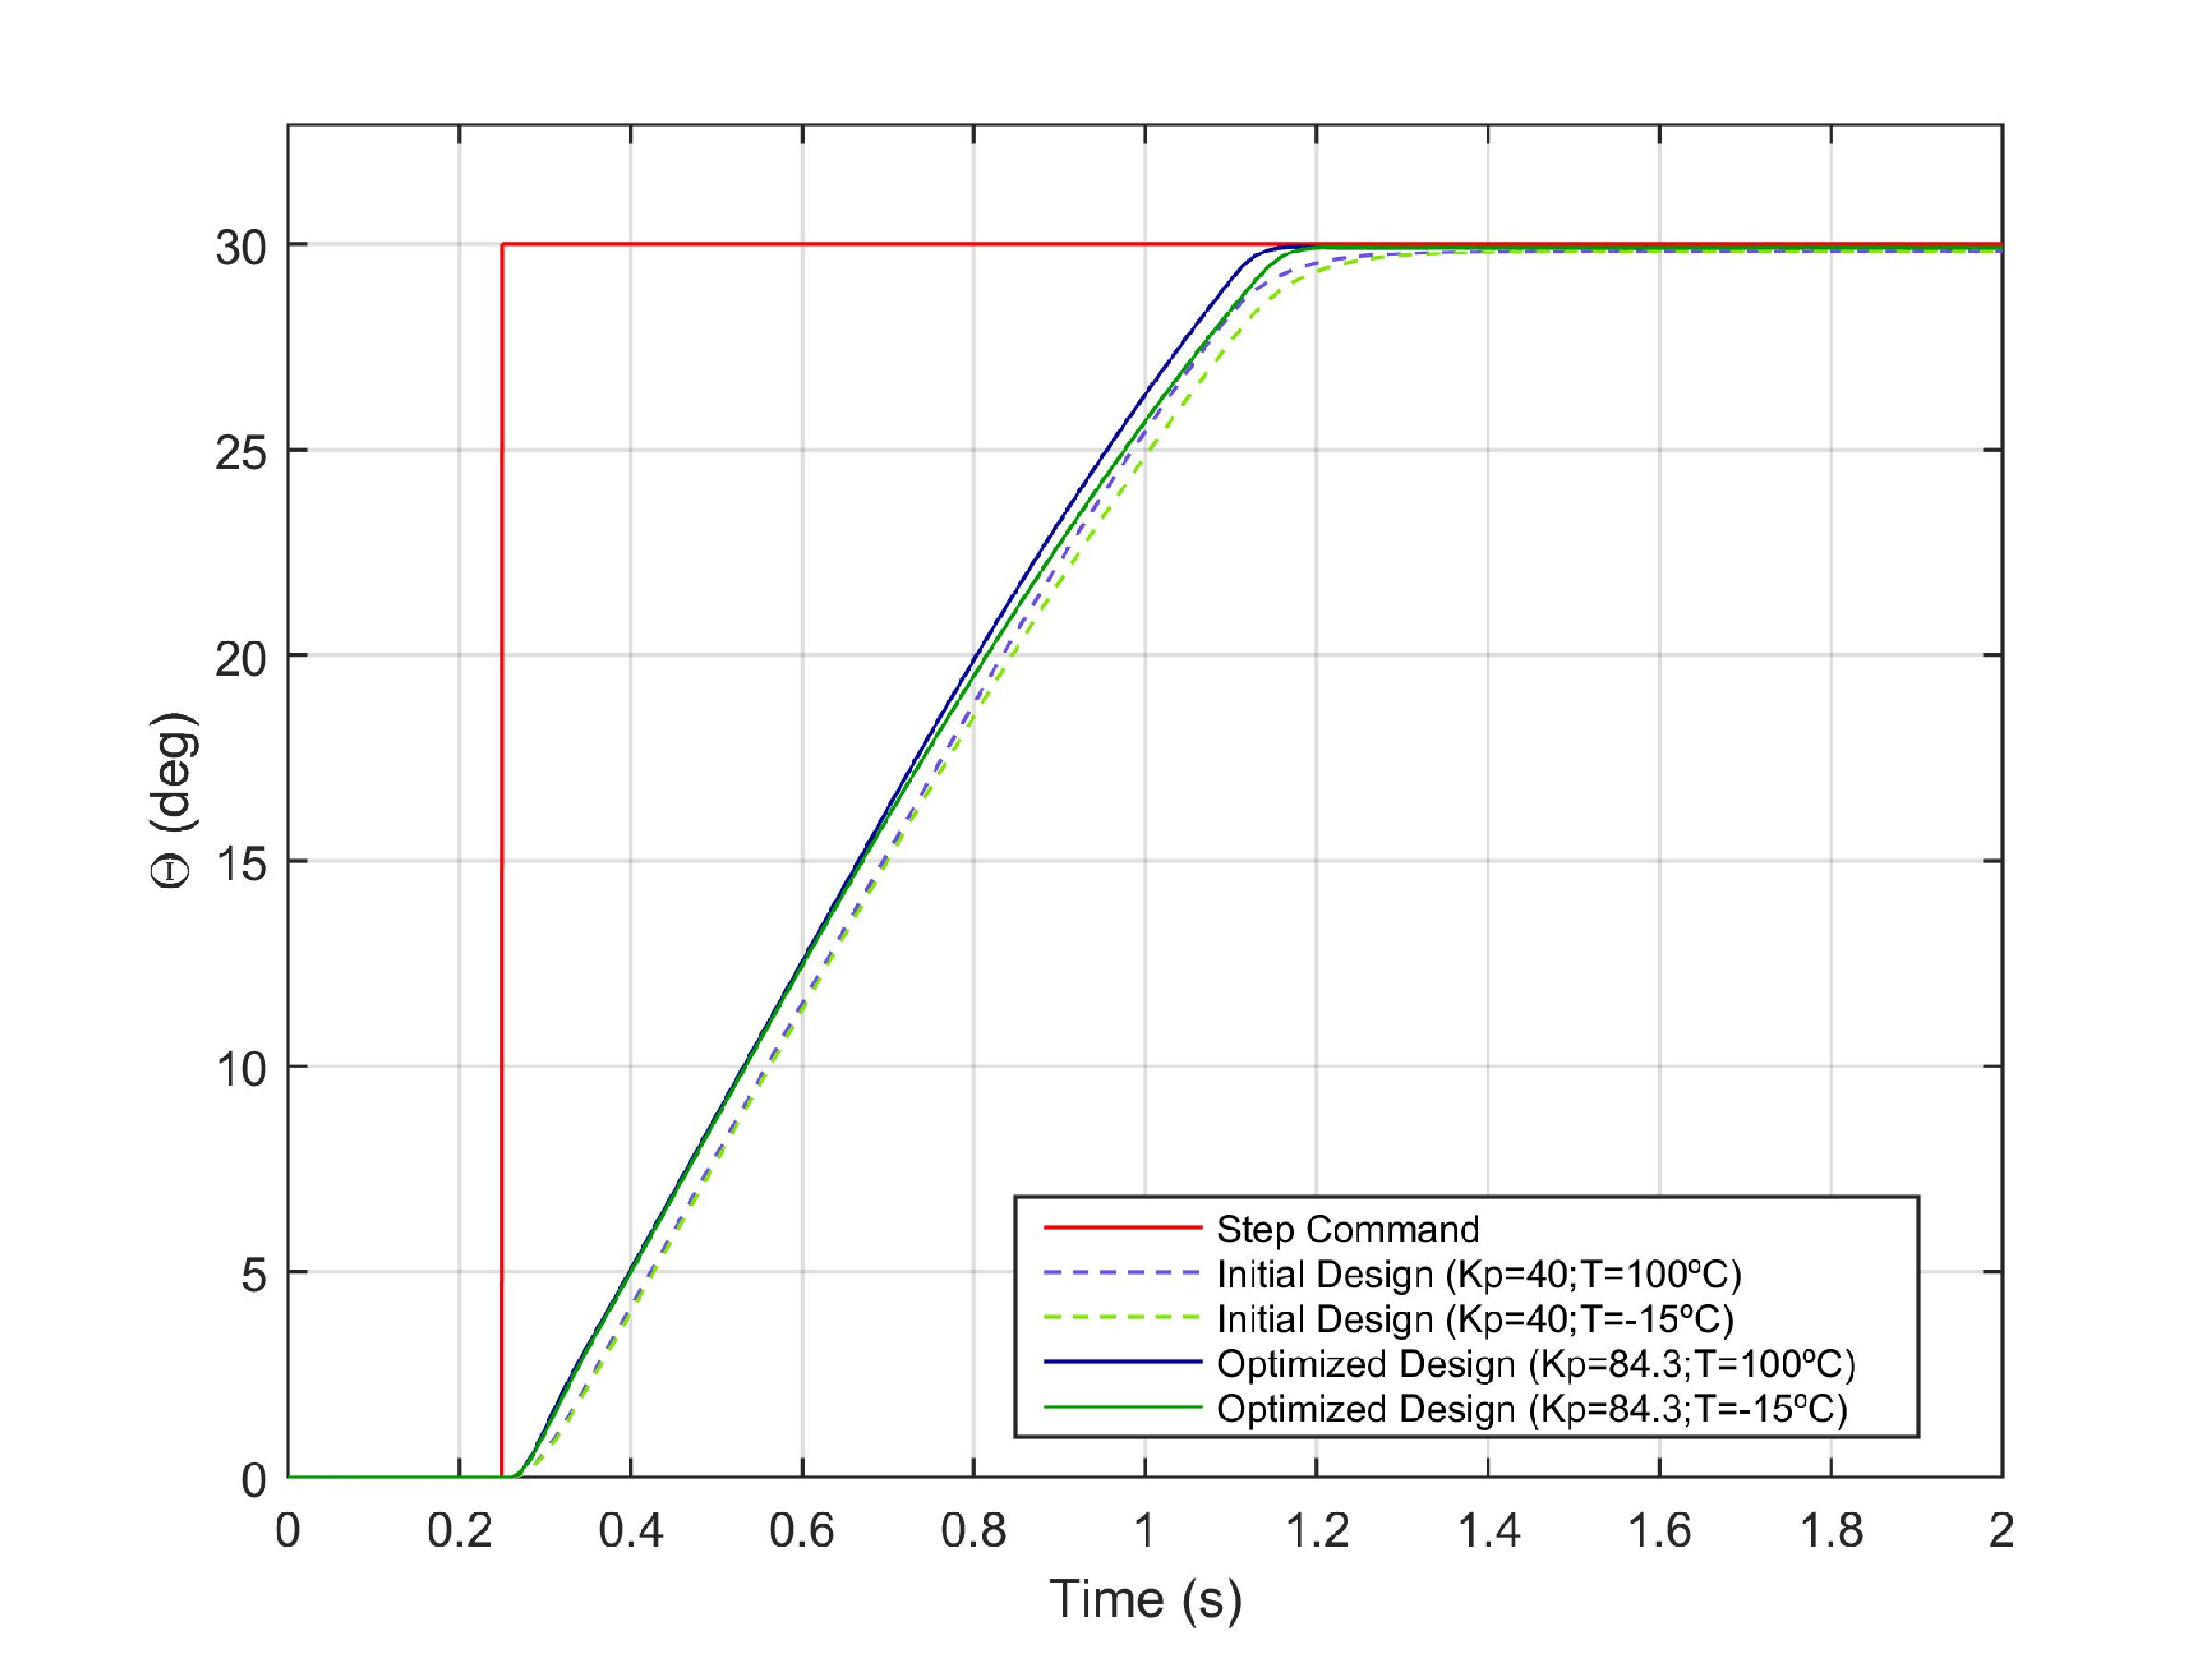
\includegraphics[width=0.9\textwidth]{Figuras/5.OptimizationResults/5-1-1-P-TimeResponseComparison.jpg}}
	\caption{Time Response Comparison for Proportional Controller.}
	\label{fig:5_1_1_P_TimeResp}
\end{figure}

\begin{figure}[H]
	\centering
	\centerline{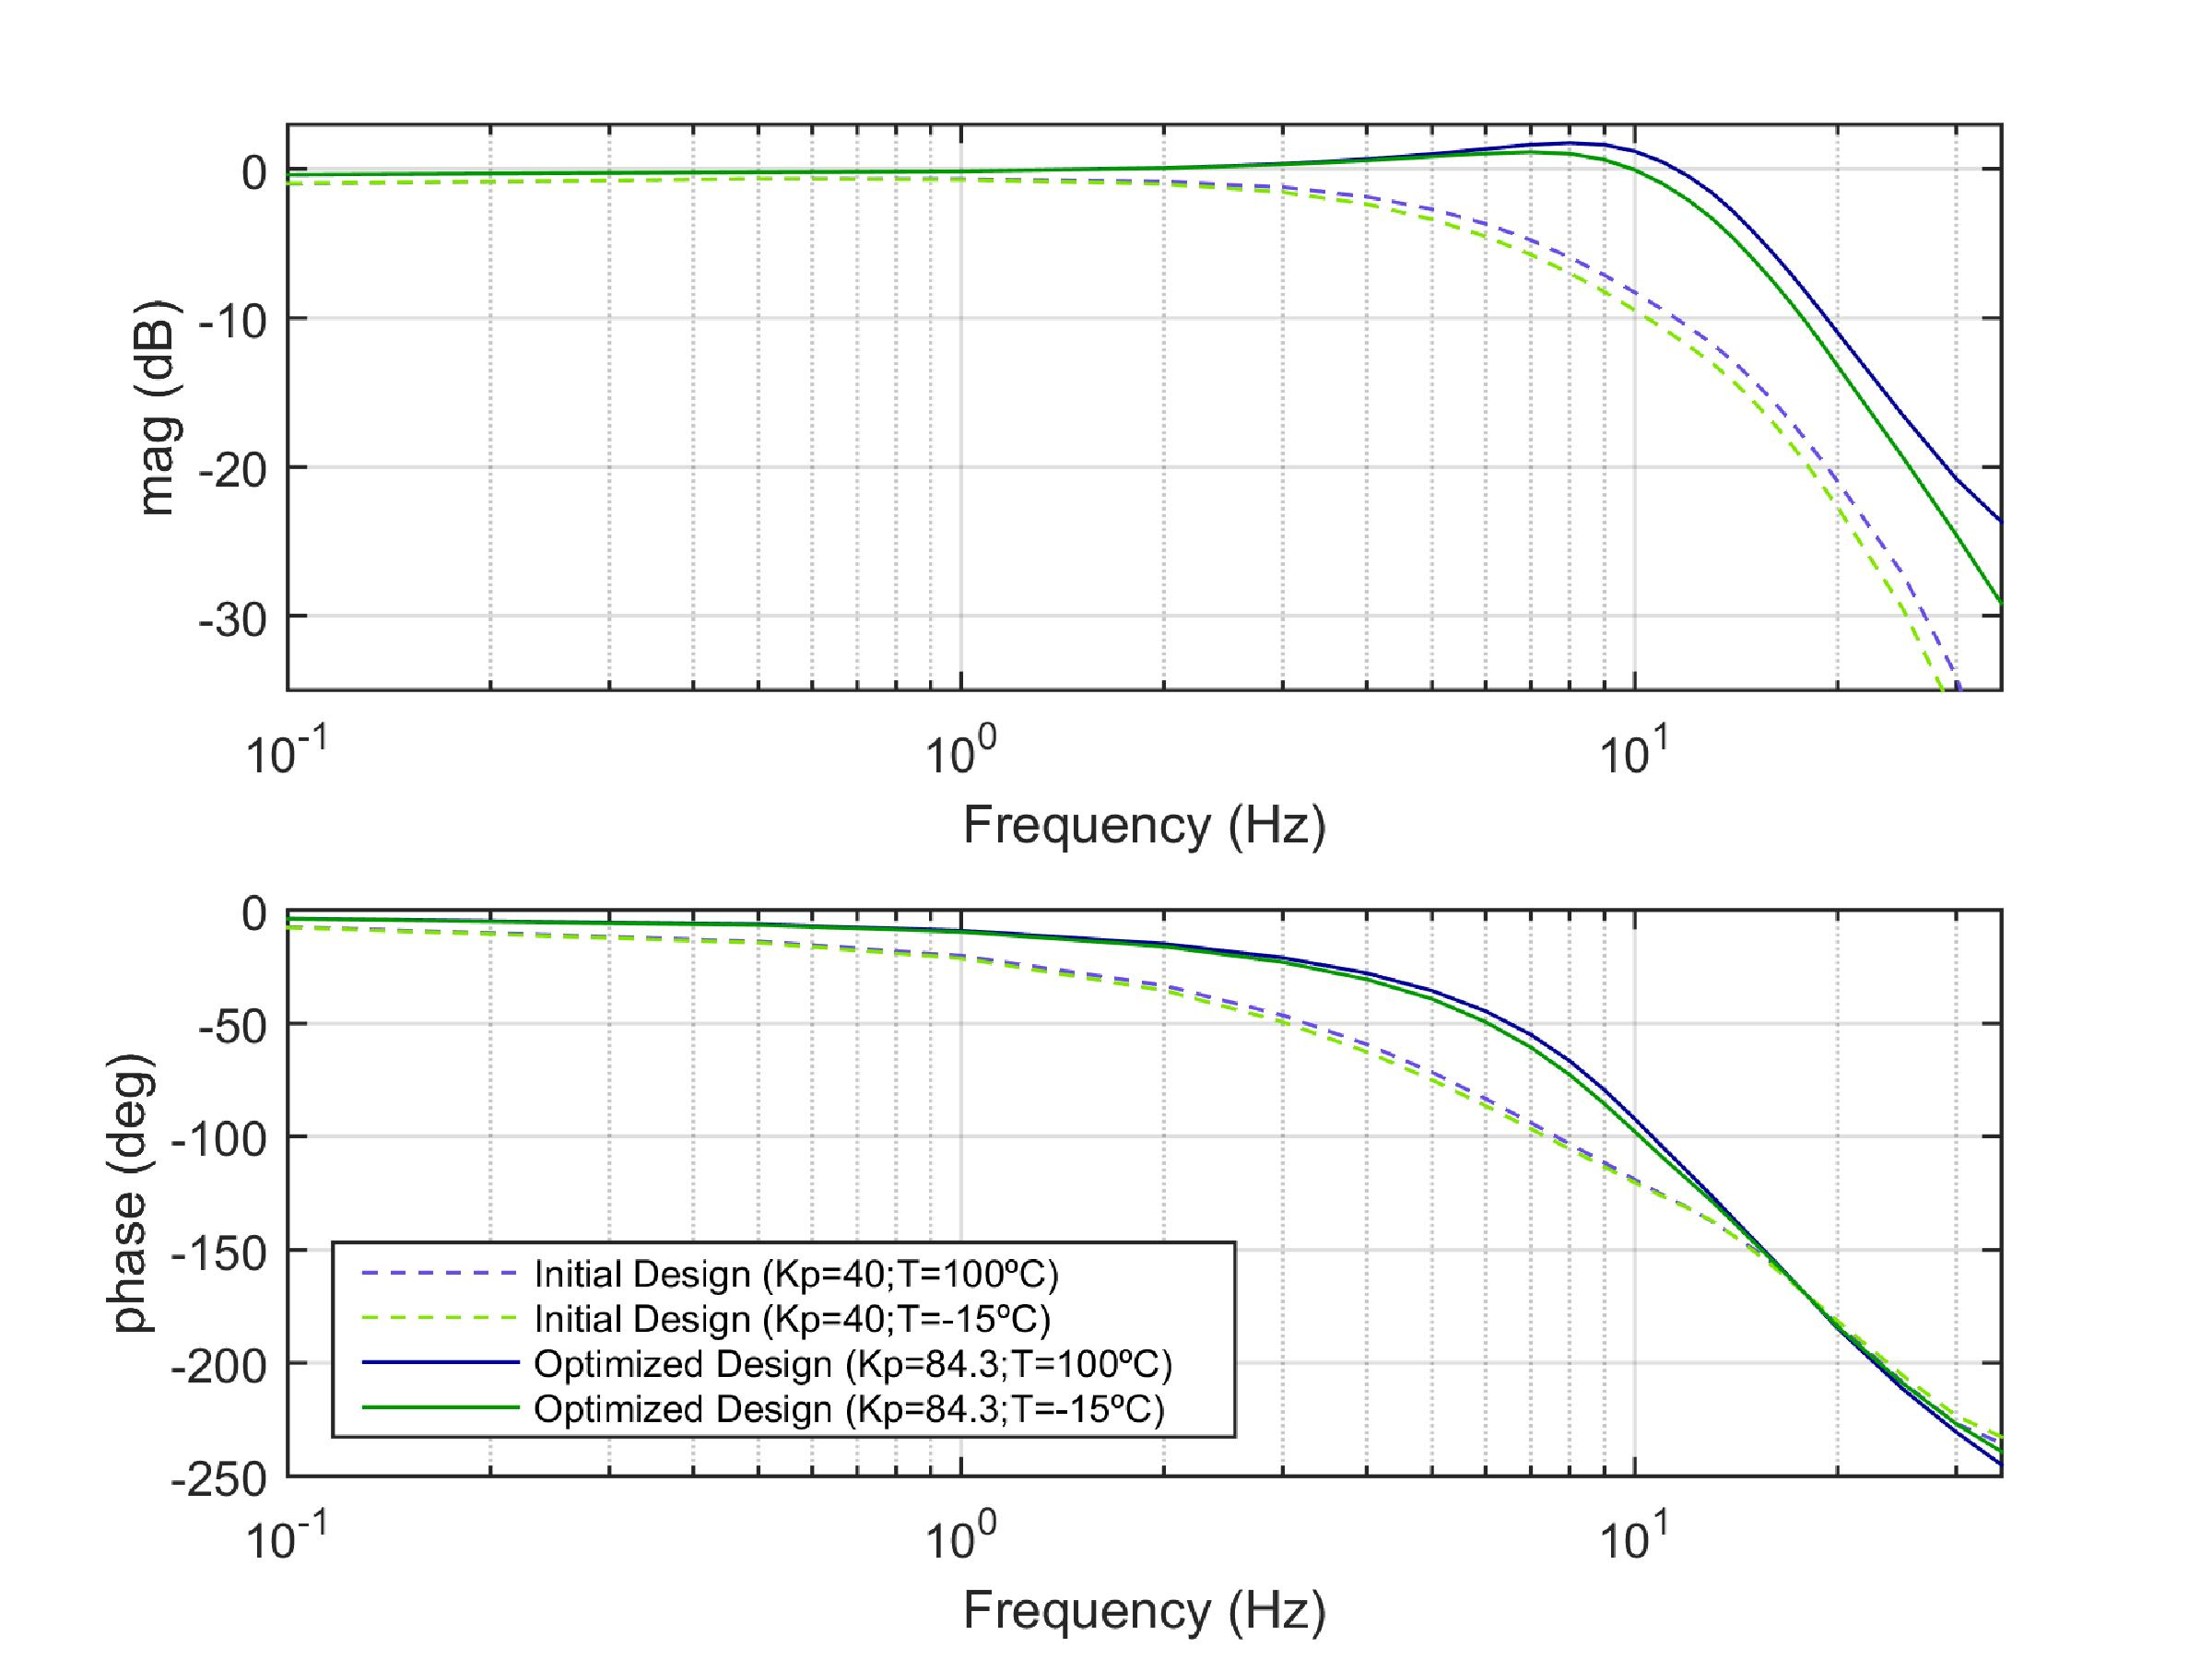
\includegraphics[width=0.9\textwidth]{Figuras/5.OptimizationResults/5-1-1-P-FrequencyResponseComparison.jpg}}
	\caption{Frequency Response Comparison for Proportional Controller.}
	\label{fig:5_1_1_P_FreqResp}
\end{figure}

The closed-loop frequency response comparison is presented in Figure \ref{fig:5_1_1_P_FreqResp} and the performance requirements are also shown in Table \ref{table:5_1_1_P_PerfTable}. The closed-loop gain and phase allowances were fairly reduced but still comply with requirements. The magnitude response surpassed 0dB and peaked at 1.75dB, above optimization constraint. Positive magnitude peaks are related to time response overshoot and dynamic stiffness reduction but in this case it did not result in any of these concerns.

\begin{table}[H]
	\captionof{table}{Requirement Compliance for Proportional Controller}
	\label{table:5_1_1_P_PerfTable}
	\centering
	\resizebox{14cm}{!} {
		\begin{tabular}{|l|c|c|c|c|}
			\hline
			Design Parameter & Requirement & Baseline & Optimized Controller & Difference (\%) \\ \hline
			Settling Time (ms) & $< 1100$ & $959$ & $891$ & $-7.1$ \\ \hline
			Steady State Error ($\%$) & $< 1$ & $0.27$ & $0.13$ & $-51.9$ \\ \hline
			Overshoot ($\%$) & $< 10 $  & $0.0$ & $0.0$ & $N/A$ \\ \hline
			Minimum Average Rate ($°/s$) & $> 32$ & $34.45$ & $34.62$ & $0.5$ \\ \hline
			Maximum Average Rate ($°/s$) & $< 36$ & $34.45$ & $34.62$ & $0.5$ \\ \hline
			Closed-Loop Gain Allowance (dB) & $ \geq 10 $ & $20.35$ & $10.13$ & $-50.2$ \\ \hline
			Closed-Loop Phase Allowance ($°$) & $ \geq 45$ & $inf$ & $69.78$ & $N/A$ \\ \hline
			Closed-Loop Maximum Peak (dB) & $ < 0.5$ & $-0.65$ & $1.75$ & $369.2$ \\ \hline
			Closed-Loop Initial Magnitude (dB) & $None$ & $-1.0$ & $-0.39$ & $61.0$ \\ \hline
			Closed-Loop Bandwidth (Hz) & $None$ & $6.30$ & $14.4$ & $128.6$ \\ \hline
	\end{tabular}}
\end{table}

\subsection{Proportional Integral Controller (PI)}

The optimization of the proportional integral controller was executed in 11.2 hours and required 19 iterations, as shown in Table \ref{table:5_1_2_PIContExecution}. Also, the optimization yielded a proportional gain of 66.88 and an integral gain of 0.001. These values also were evaluated by \citeonline{Ballesteros} and similar behavior in this case is expected as well. 

\begin{table}[H]
	\captionof{table}{PI Controller Optimization Execution Results}
	\label{table:5_1_2_PIContExecution}
	\centering
	\resizebox{7cm}{!} {
		\begin{tabular}{|l|c|}
			\hline
			Optimized Proportional Gain & 66.88 \\ \hline
			Optimized Integral Gain & 0.001 \\ \hline
			Optimization Execution Time (h) & 11.2 \\ \hline
			Number of Iterations & 19 \\ \hline			
			Number of Obj. Function Evaluations & 68 \\ \hline	
	\end{tabular}}
\end{table}

The  dynamic stiffness response for each PI design is shown in Figure \ref{fig:5_1_2_PI_DynStif}. Similarly to the P controller, increase in dynamic stiffness was observed only in frequencies below 4Hz and a decrease occurred for frequencies between 4Hz and 15Hz.

\begin{figure}[H]
	\centering
	\centerline{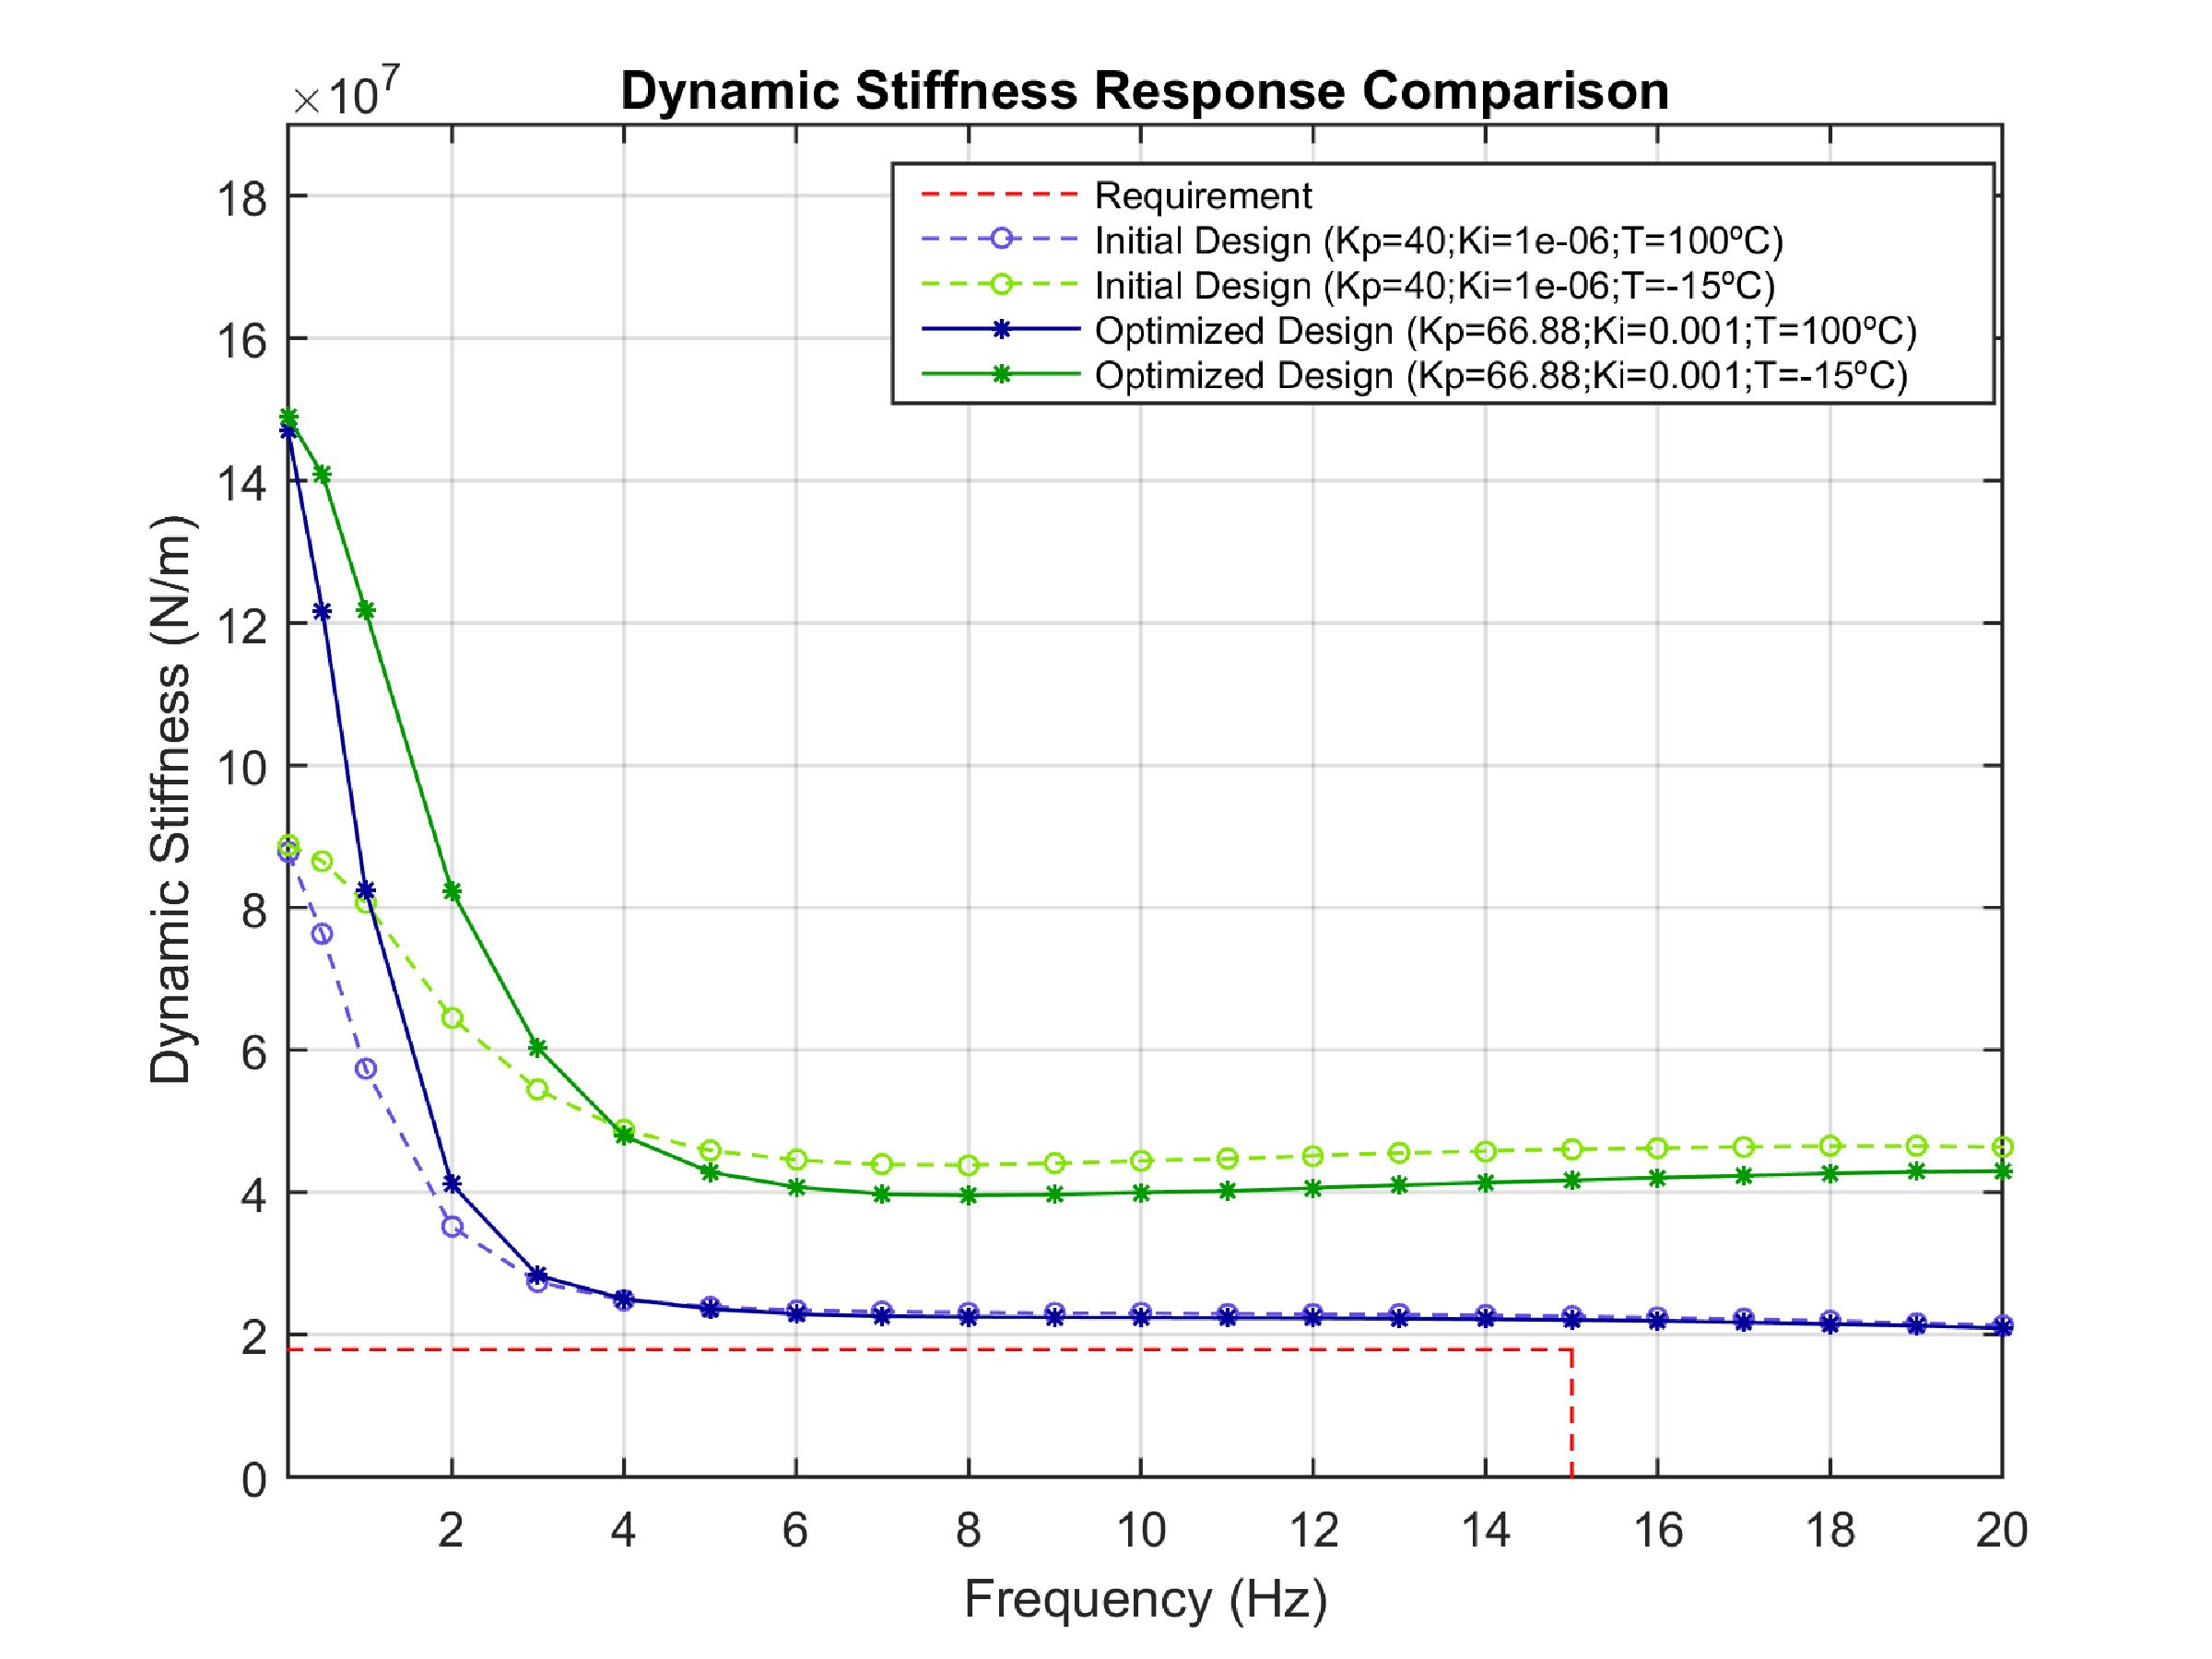
\includegraphics[width=0.9\textwidth]{Figuras/5.OptimizationResults/5-1-2-PI-DynamicStiffnessComparison.jpg}}
	\caption{Dynamic Stiffness Optimization Result for the PI Controller.}
	\label{fig:5_1_2_PI_DynStif}
\end{figure}

Table \ref{table:5_1_2_PI_CostFunctionTable} show the partial values of the cost function for each frequency evaluated by the dynamic stiffness test. The lower frequencies values are considerably larger since stiffness increase occurred in this range. 

\begin{table}[H]
	\captionof{table}{PI Controller Final Solution Cost Function for Each Evaluated Frequency}
	\label{table:5_1_2_PI_CostFunctionTable}
	\centering
	\resizebox{14cm}{!} {
		\begin{tabular}{|c|c|c|c|c|c|}
			\hline
			Frequency (Hz) & $J_i$ & Frequency (Hz) & $J_i$ & Frequency (Hz) & $J_i$ \\ \hline
			$0.1$ & $1.29e+08$ & $5$ & $5.72e+06$ & $11$ & $4.46e+06$ \\ \hline
			$0.5$ & $1.04e+08$ & $6$ & $5.01e+06$ & $12$ & $4.44e+06$ \\ \hline
			$1$ & $6.46e+07$ & $7$ & $4.67e+06$ & $13$ & $4.38e+06$ \\ \hline
			$2$ & $2.32e+07$ & $8$ & $4.58e+06$ & $14$ & $4.29e+06$ \\ \hline
			$3$ & $1.04e+07$ & $9$ & $4.54e+06$ & $15$ & $4.15e+06$ \\ \hline
			$4$ & $7.12e+06$ & $10$ & $4.5e+06$ &  &  \\ \hline
	\end{tabular}}
\end{table}

The time response comparison is presented in Figure \ref{fig:5_1_2_PI_TimeResp} and the performance requirements are shown in Table \ref{table:5_1_2_PI_PerfTable}. The settling time decreased by 57ms and the steady state error decreased almost 40\%.

\begin{figure}[H]
	\centering
	\centerline{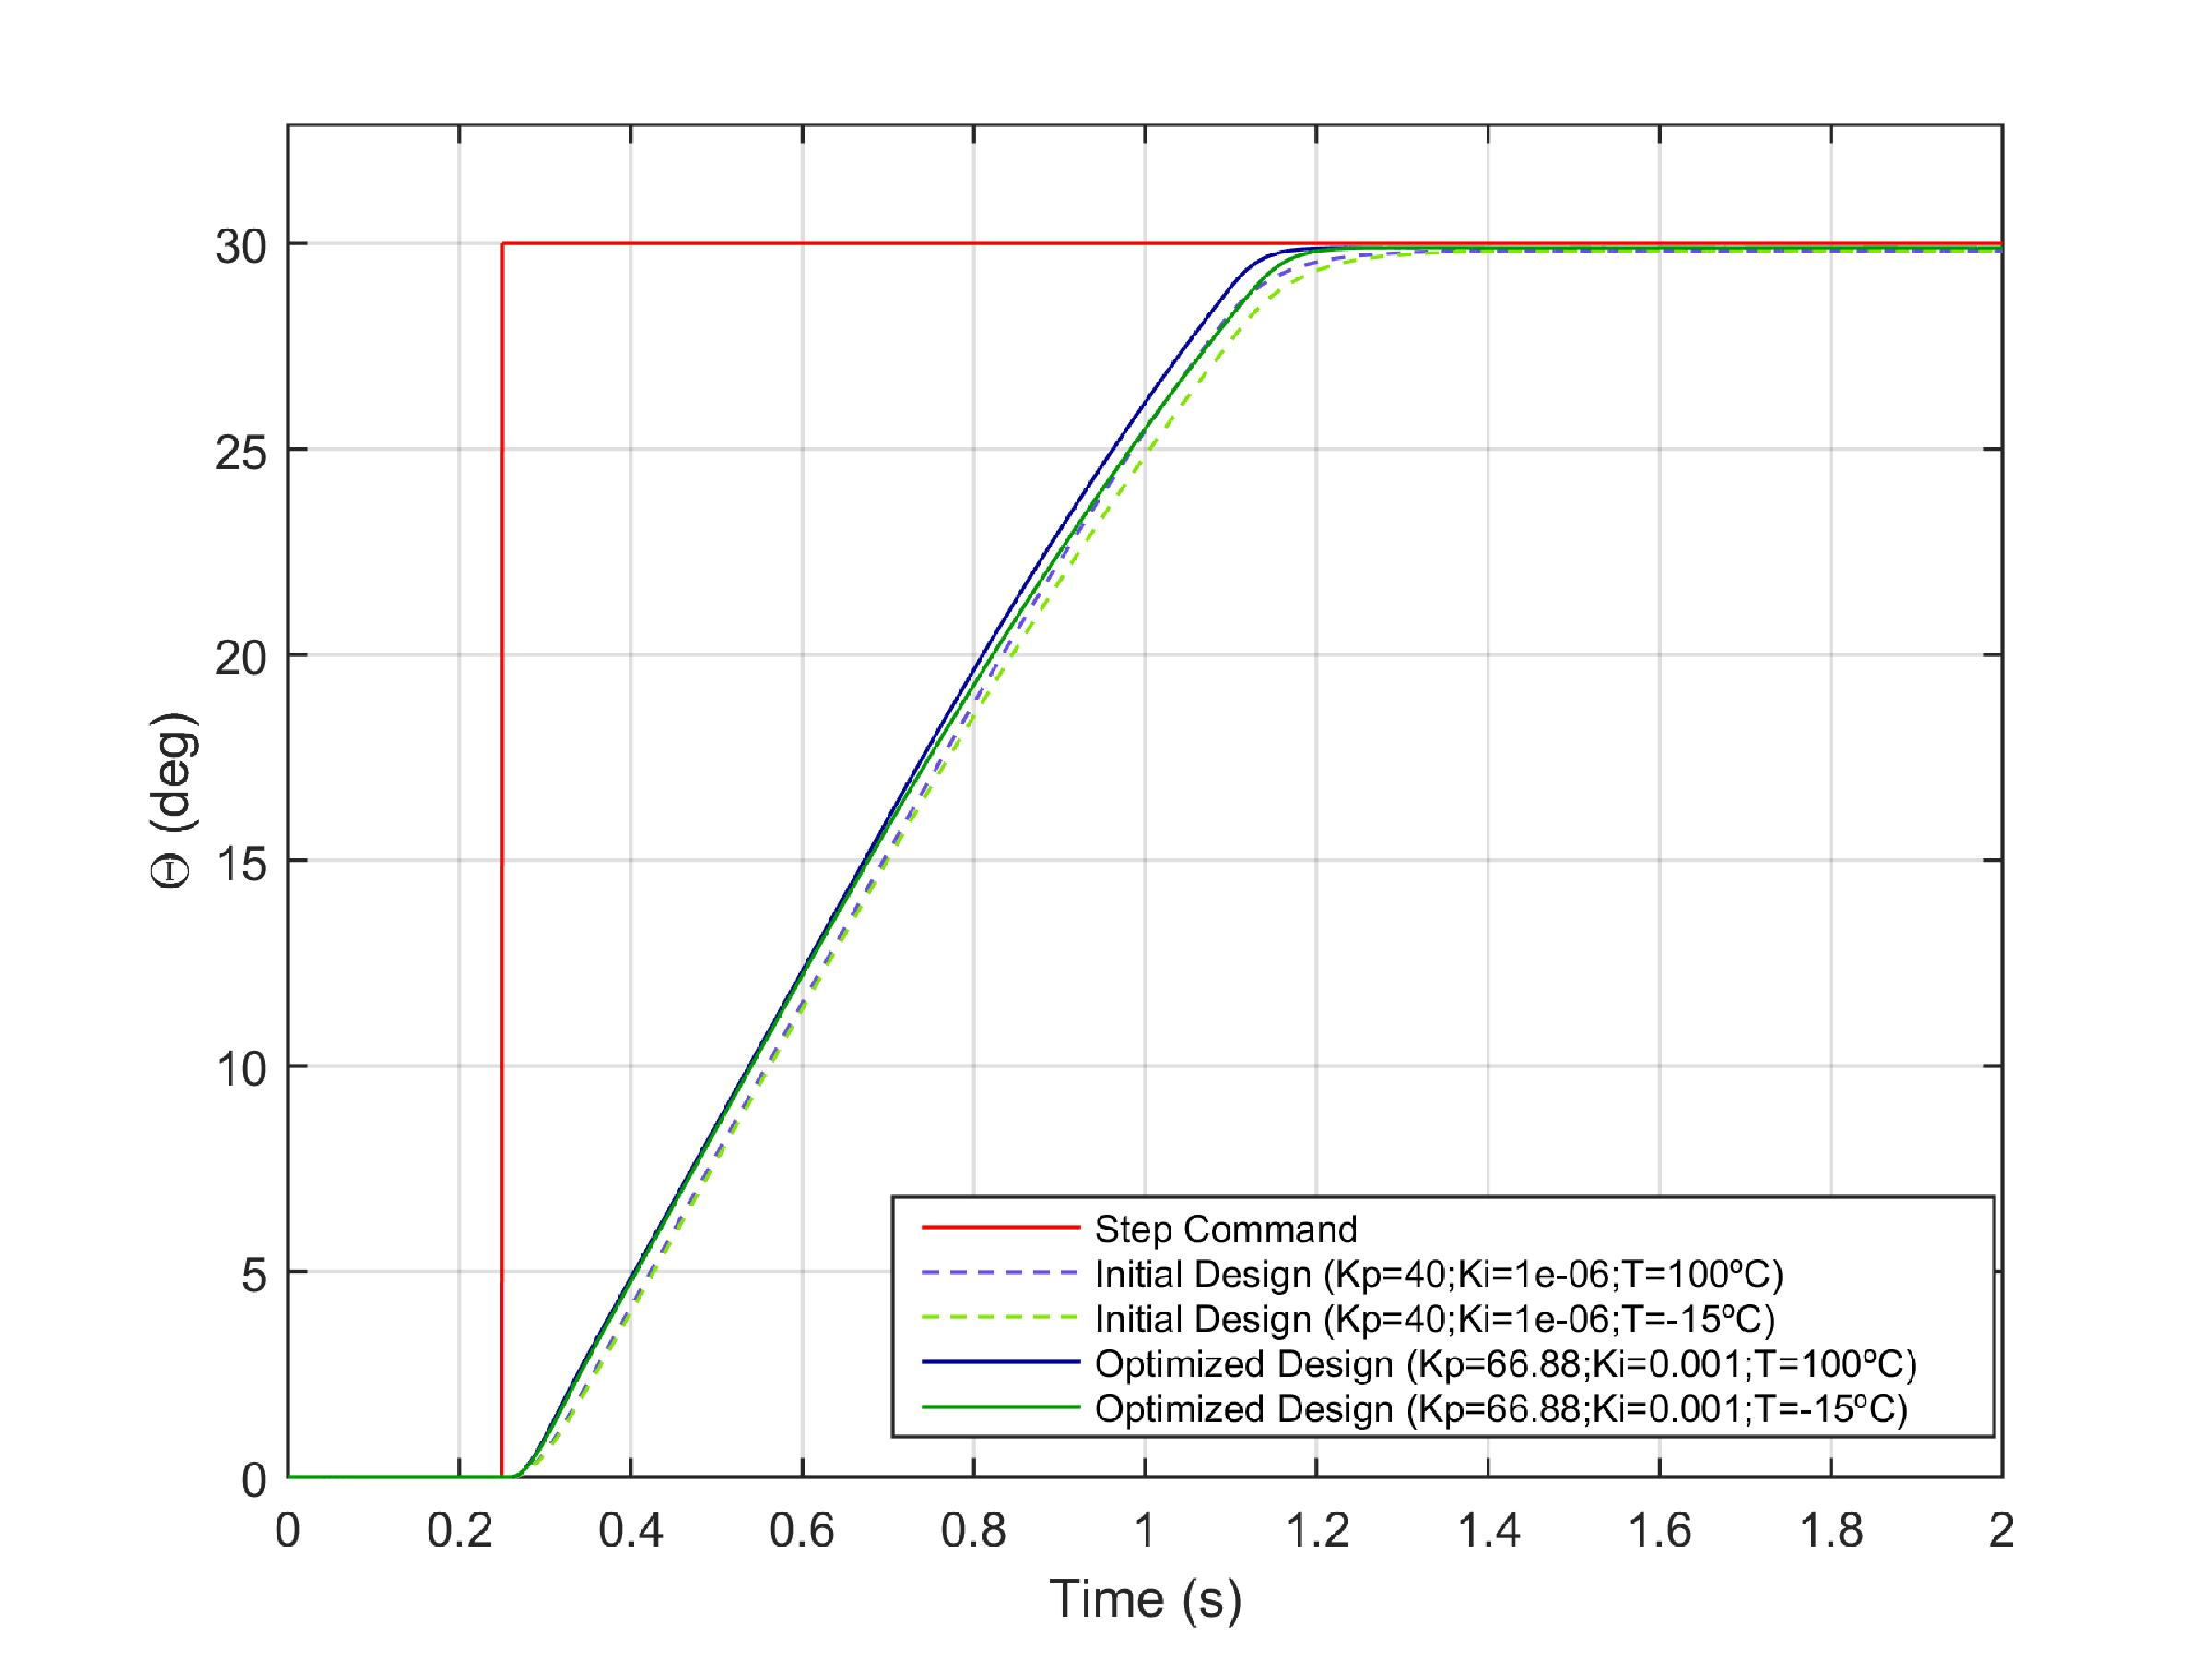
\includegraphics[width=0.9\textwidth]{Figuras/5.OptimizationResults/5-1-2-PI-TimeResponseComparison.jpg}}
	\caption{Time Response Optimization Result for the PI Controller.}
	\label{fig:5_1_2_PI_TimeResp}
\end{figure}

The closed-loop frequency response comparison is presented in Figure \ref{fig:5_1_2_PI_FreqResp} and the performance requirements are also shown in Table \ref{table:5_1_2_PI_PerfTable}. The closed-loop gain and phase allowances were fairly reduced but still comply with requirements. The magnitude response surpassed 0 dB and peaked at 0.41 dB, just below the 0.5dB requirement.

\begin{figure}[H]
	\centering
	\centerline{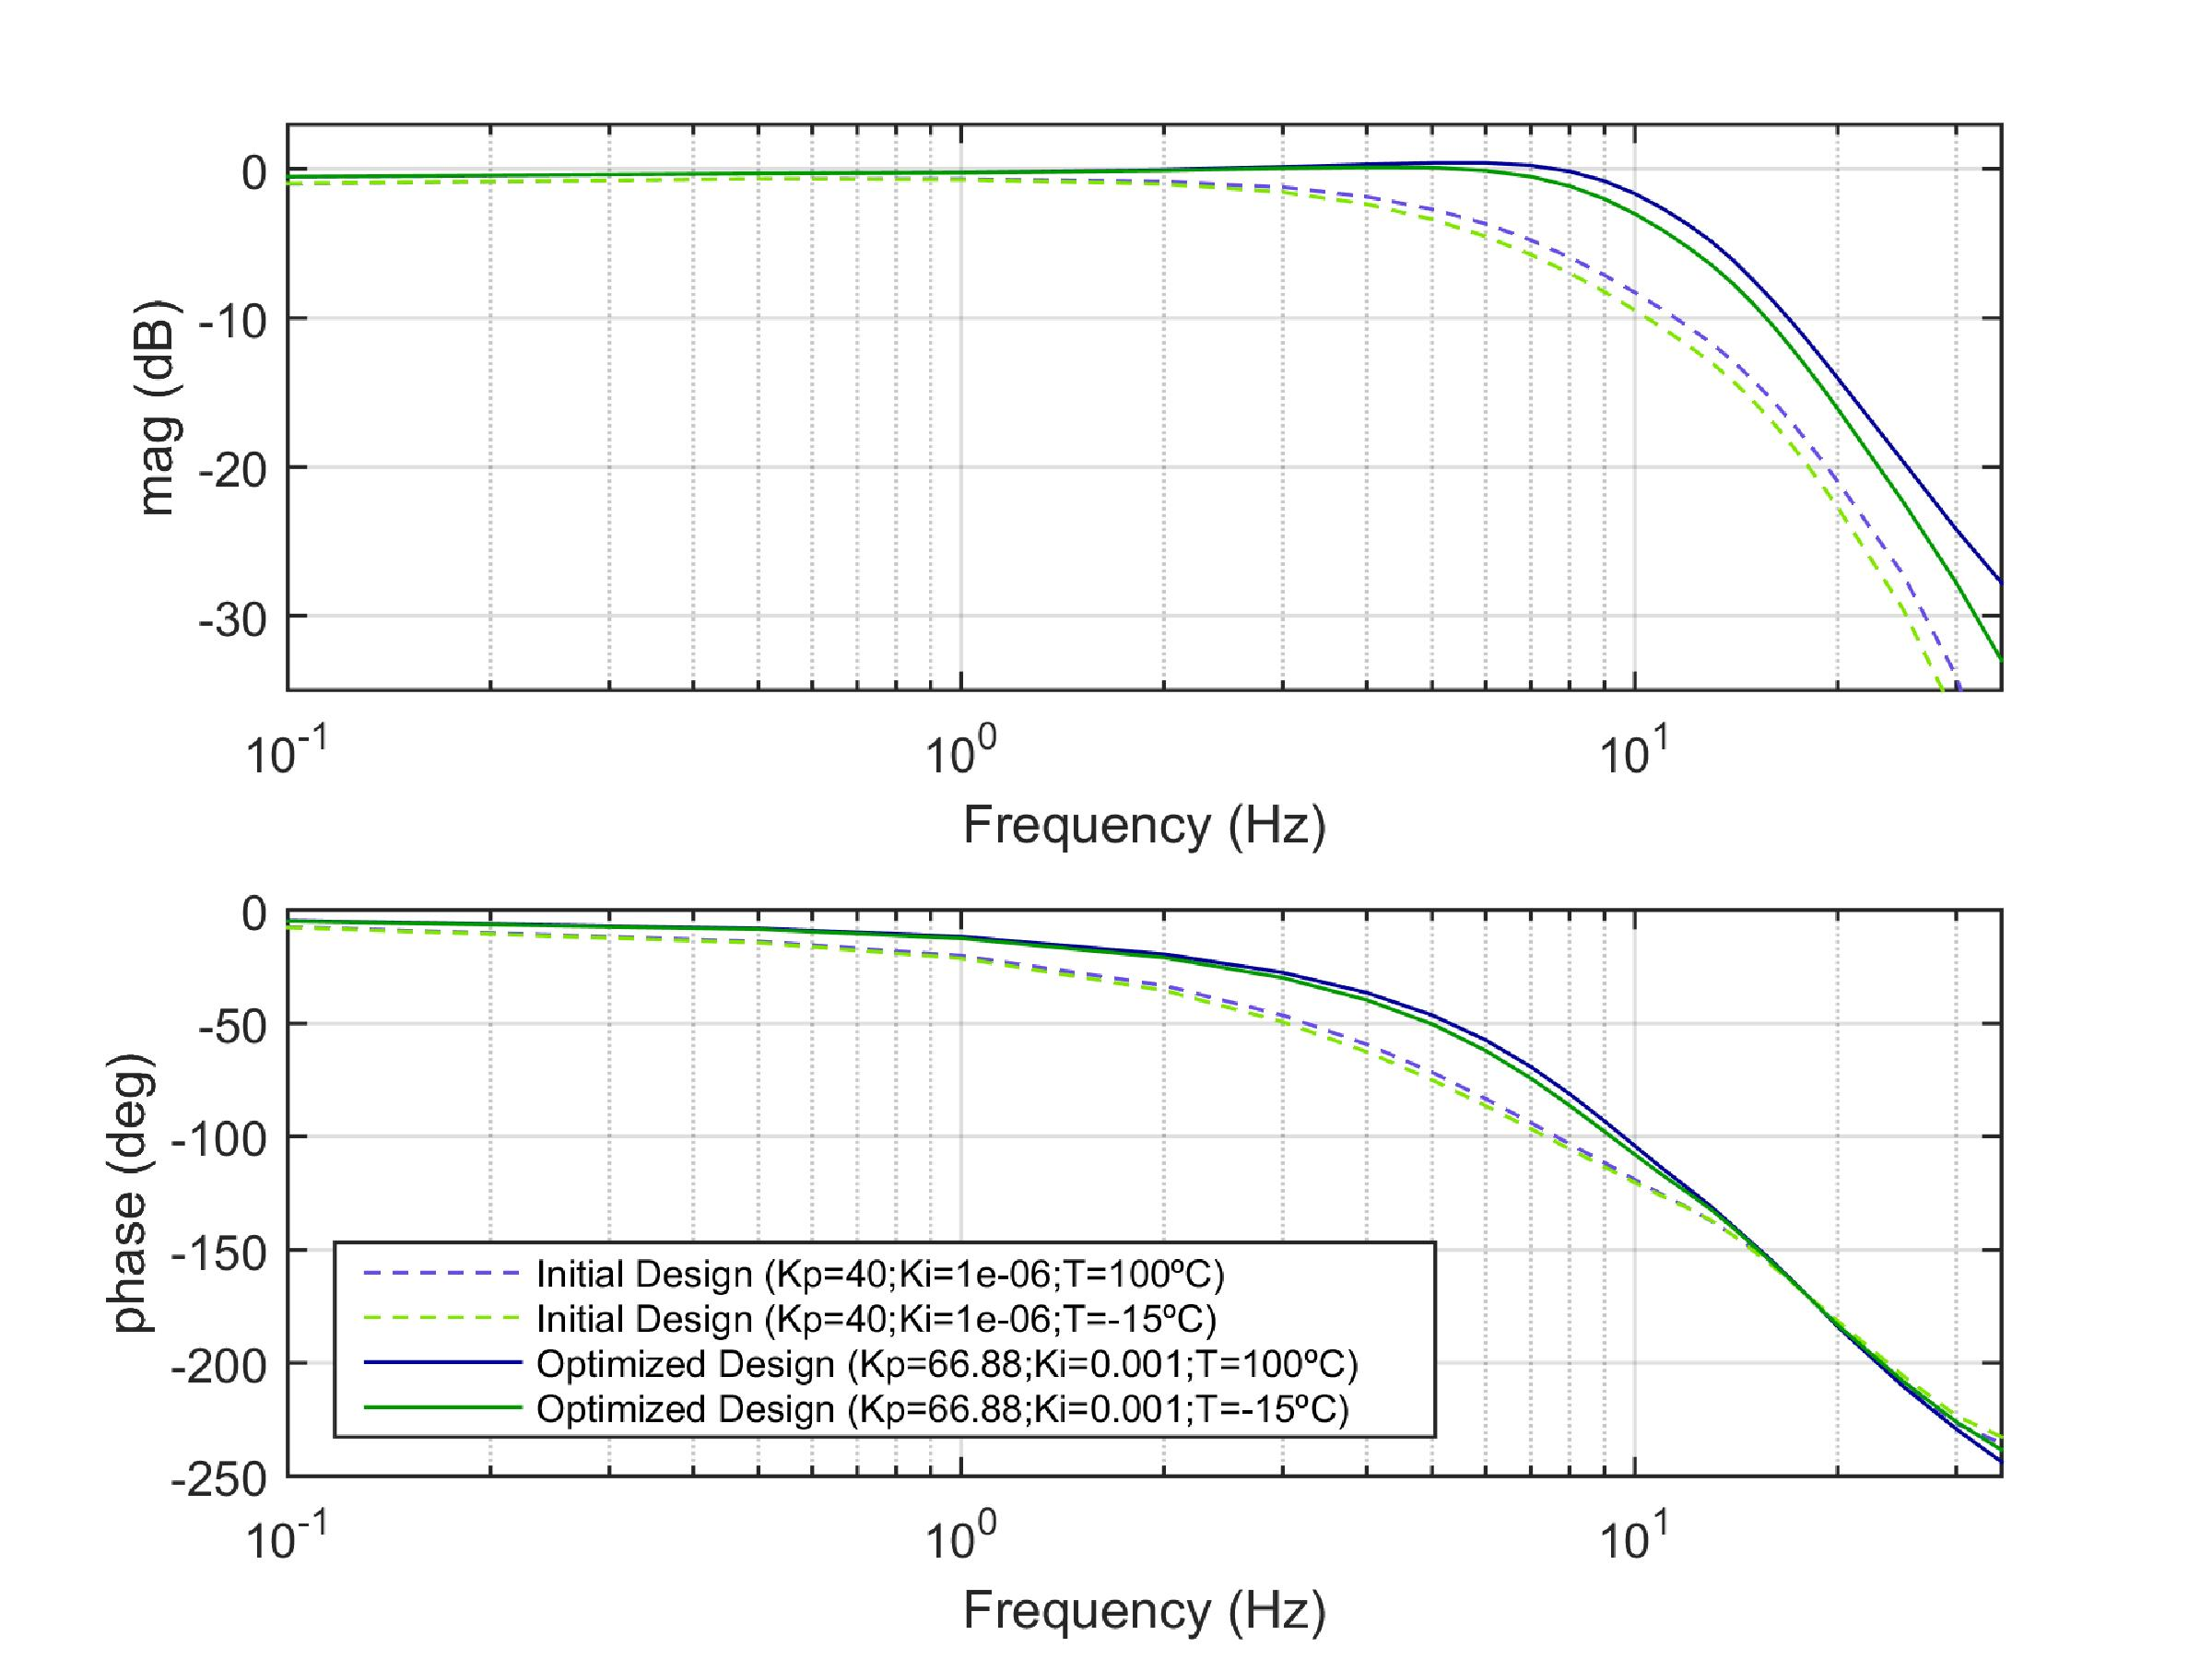
\includegraphics[width=0.9\textwidth]{Figuras/5.OptimizationResults/5-1-2-PI-FrequencyResponseComparison.jpg}}
	\caption{Frequency Response Baseline for the PI Controller.}
	\label{fig:5_1_2_PI_FreqResp}
\end{figure}

\begin{table}[H]
	\captionof{table}{Requirement Compliance for PI Controller}
	\label{table:5_1_2_PI_PerfTable}
	\centering
	\resizebox{14cm}{!} {
		\begin{tabular}{|l|c|c|c|c|}
			\hline
			Design Parameter & Requirement & Baseline & Optimized Controller & Difference (\%) \\ \hline
			Settling Time (ms) & $< 1100 $ & $959$ & $902$ & $-5.9.$ \\ \hline
			Steady State Error ($\%$) & $< 1$ & $0.27$ & $0.16$ & $-40.7$ \\ \hline
			Overshoot ($\%$) & $< 10 $  & $0.0$ & $0.0$ & $N/A$ \\ \hline
			Minimum Average Rate ($°/s$) & $> 32$ & $34.45$ & $34.58$ & $0.4$ \\ \hline
			Maximum Average Rate ($°/s$) & $< 36$ & $34.45$ & $34.58$ & $0.4$ \\ \hline
			Closed-Loop Gain Allowance (dB) & $ \geq 10 $ & $20.34$ & $13.31$ & $-34.6.$ \\ \hline
			Closed-Loop Phase Allowance ($°$) & $ \geq 45$ & $inf$ & $103.6$ & $N/A$ \\ \hline
			Closed-Loop Maximum Peak (dB) & $ < 0.5$ & $-0.65$ & $0.41$ & $163.1$ \\ \hline
			Closed-Loop Initial Magnitude (dB) & $None$ & $-1.0$ & $-0.52$ & $48.0$ \\ \hline
			Closed-Loop Bandwidth (Hz) & $None$ & $6.30$ & $11.80$ & $87.3$ \\ \hline
	\end{tabular}}
\end{table}

\subsection{Proportional Derivative Controller (PD)}

The proportional derivative controller optimization execution time was 18 hours and required 32 iterations, as per Table \ref{table:5_1_3_PDContExecution}. Also, the optimization yielded a proportional gain of 79.59 and a derivative gain of 0.3339. These values also were evaluated by \citeonline{Ballesteros} and similar behavior in this case is expected as well. 

\begin{table}[H]
	\captionof{table}{PD Controller Optimization Execution Results}
	\label{table:5_1_3_PDContExecution}
	\centering
	\resizebox{7cm}{!} {
		\begin{tabular}{|l|c|}
			\hline
			Optimized Proportional Gain & 79.59 \\ \hline
			Optimized Derivative Gain & 0.3339 \\ \hline
			Optimization Execution Time (h) & 18.0 \\ \hline
			Number of Iterations & 32 \\ \hline		
			Number of Obj. Function Evaluations & 121 \\ \hline		
	\end{tabular}}
\end{table}

The  dynamic stiffness response for each PD design is shown in Figure \ref{fig:5_1_3_PD_DynStif}. Similarly to previous controllers, the dynamic stiffness increase was restricted to frequencies below 3Hz but, for the PD, a fair reduction was observed in higher frequencies. This behavior is coherent with $K_d$ parametric study which demonstrated dynamic stiffness reduction for frequencies below 12Hz \cite{Ballesteros}.

\begin{figure}[H]
	\centering
	\centerline{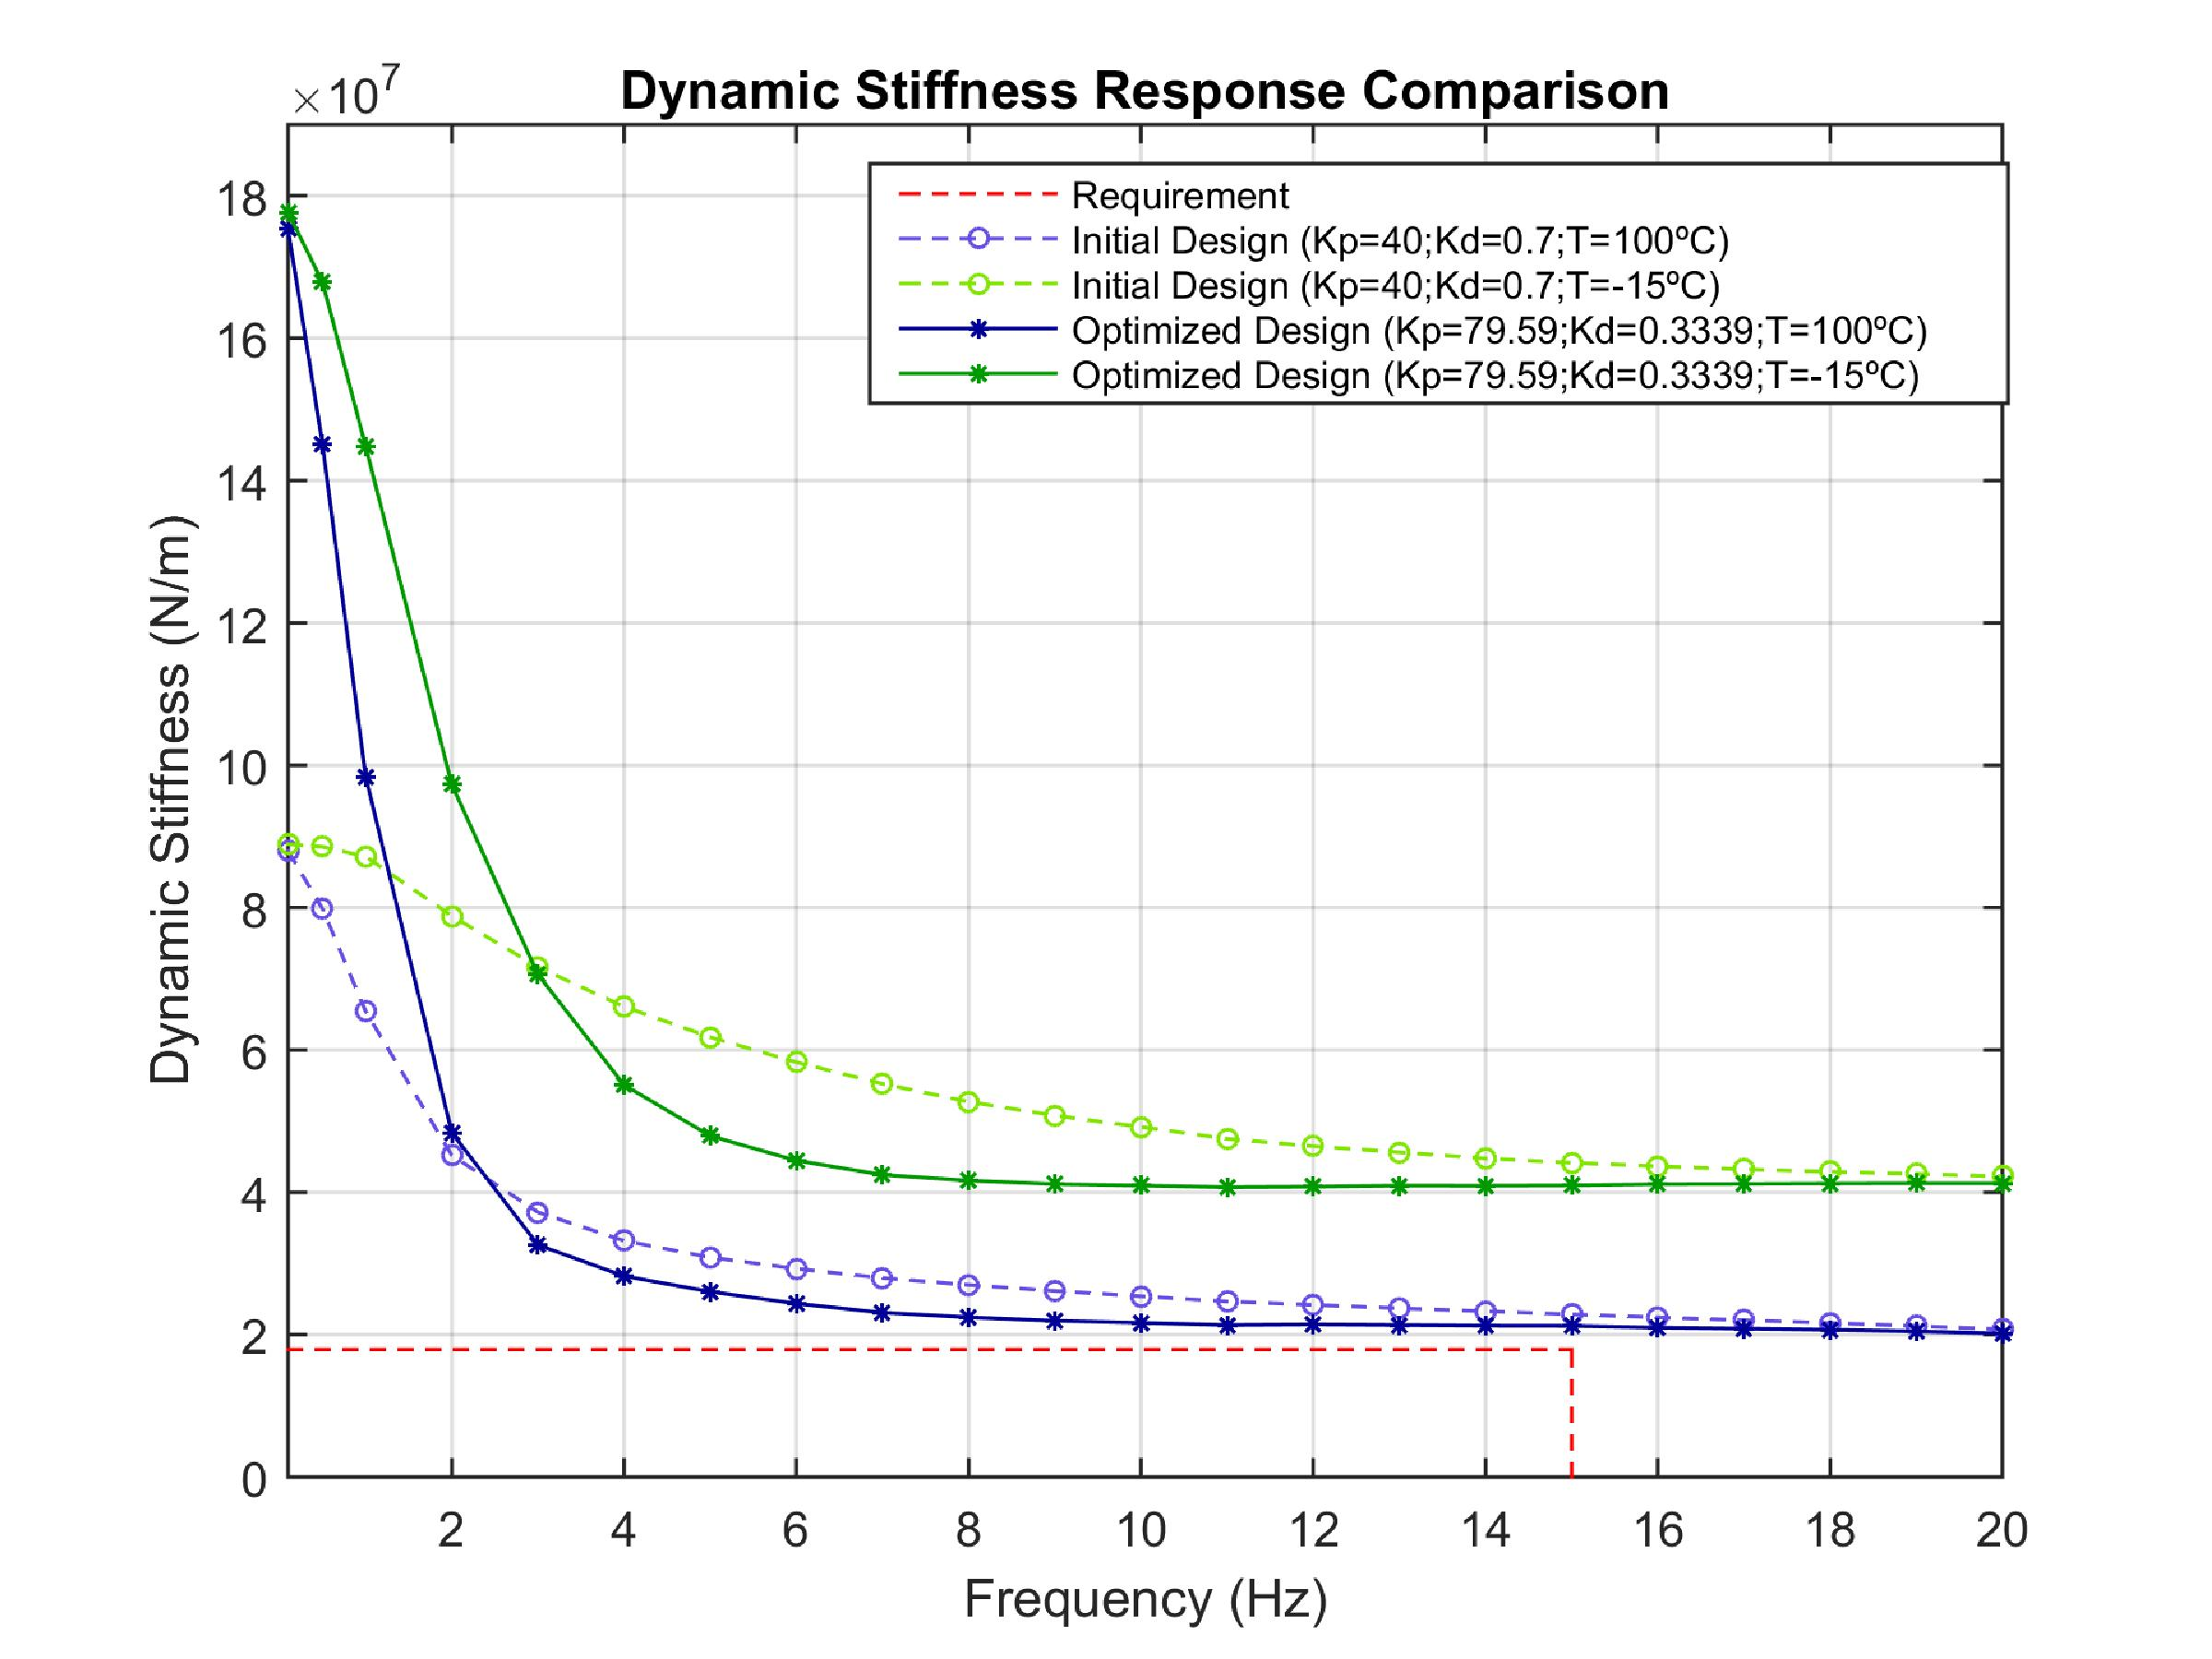
\includegraphics[width=0.9\textwidth]{Figuras/5.OptimizationResults/5-1-3-PD-DynamicStiffnessComparison.jpg}}
	\caption{Dynamic Stiffness Optimization Result for the PD Controller.}
	\label{fig:5_1_3_PD_DynStif}
\end{figure}

Table \ref{table:5_1_3_PD_CostFunctionTable} show the partial values of the cost function for each frequency evaluated by the dynamic stiffness test. The lower frequencies values are considerably larger since stiffness increase occurred in this range. 

\begin{table}[H]
	\captionof{table}{PD Controller Final Solution Cost Function for Each Evaluated Frequency}
	\label{table:5_1_3_PD_CostFunctionTable}
	\centering
	\resizebox{14cm}{!} {
		\begin{tabular}{|c|c|c|c|c|c|}
			\hline
			Frequency (Hz) & $J_i$ & Frequency (Hz) & $J_i$ & Frequency (Hz) & $J_i$ \\ \hline
			$0.1$ & $1.57e+08$ & $5$ & $8.14e+06$ & $11$ & $3.45e+06$ \\ \hline
			$0.5$ & $1.27e+08$ & $6$ & $6.47e+06$ & $12$ & $3.55e+06$ \\ \hline
			$1$ & $8.05e+07$ & $7$ & $5.19e+06$ & $13$ & $3.46e+06$ \\ \hline
			$2$ & $3.05e+07$ & $8$ & $4.54e+06$ & $14$ & $3.36e+06$ \\ \hline
			$3$ & $1.47e+07$ & $9$ & $4.06e+06$ & $15$ & $3.33e+06$ \\ \hline
			$4$ & $1.03e+07$ & $10$ & $3.77e+06$ &  &  \\ \hline
	\end{tabular}}
\end{table}

The time response comparison is presented in Figure \ref{fig:5_1_3_PD_TimeResp} and the performance requirements are shown in Table \ref{table:5_1_3_PD_PerfTable}. The settling time decreased by 97ms and the steady state error decreased almost 50\%.

\begin{figure}[H]
	\centering
	\centerline{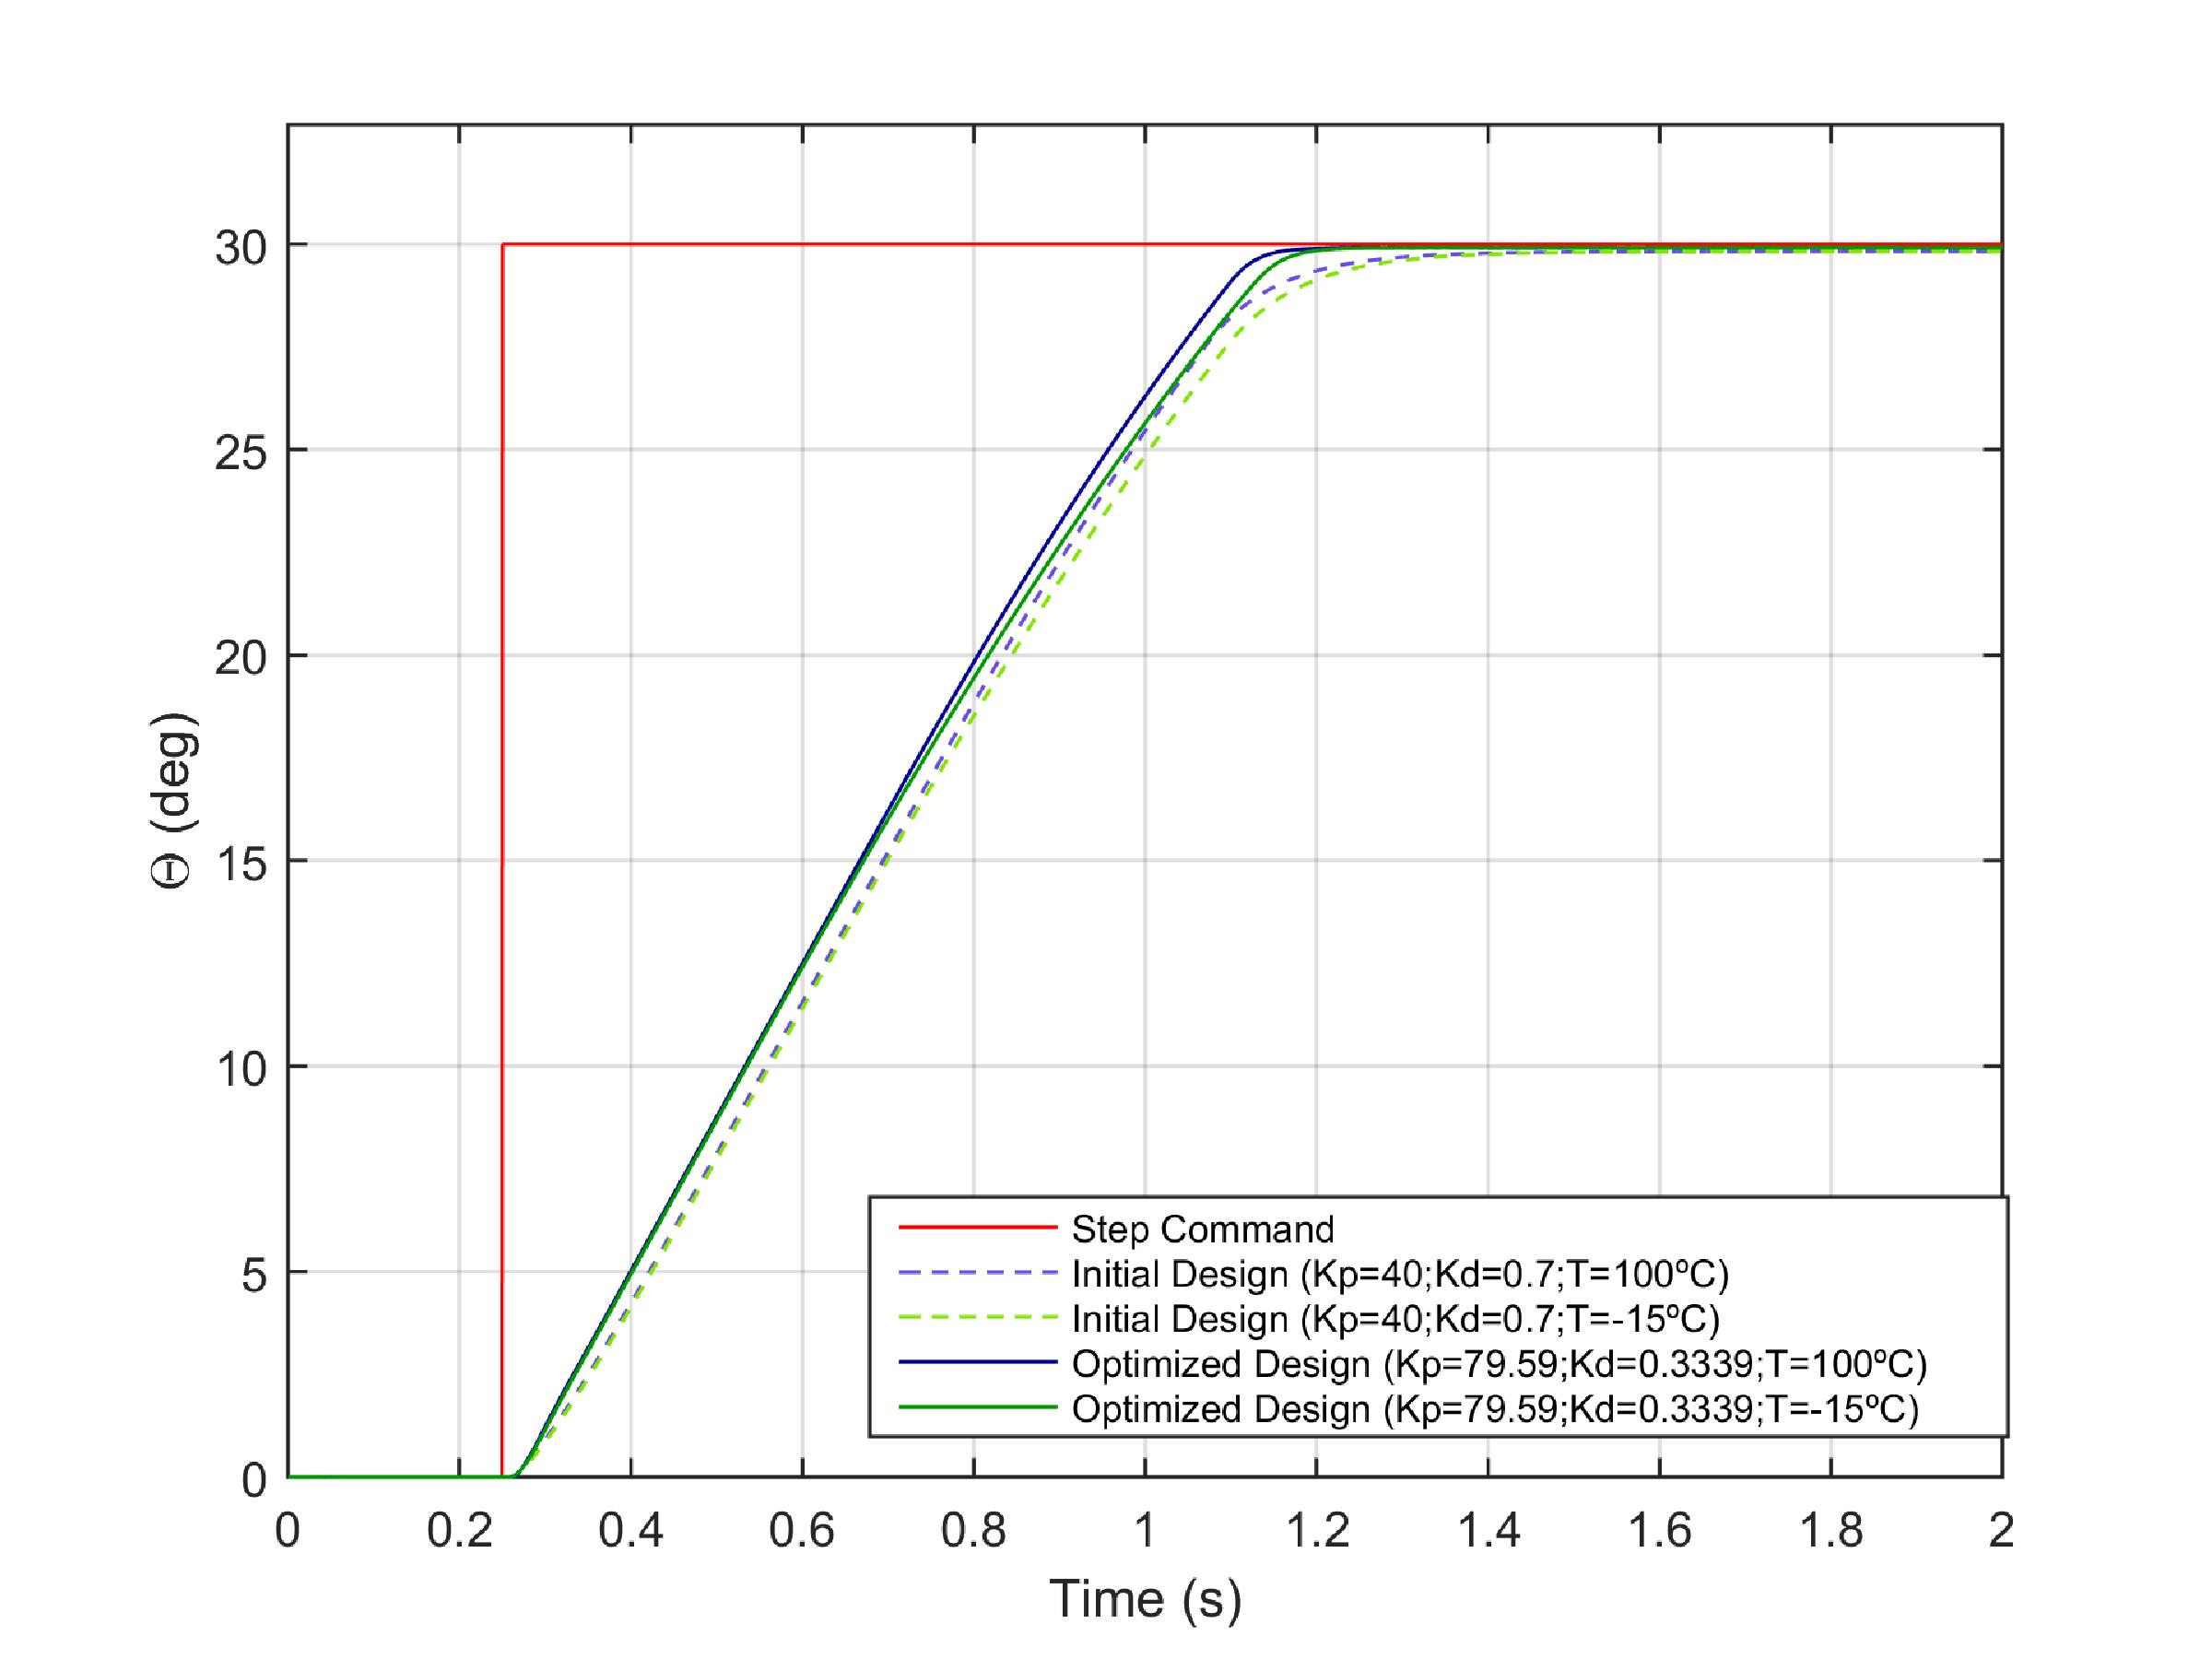
\includegraphics[width=0.9\textwidth]{Figuras/5.OptimizationResults/5-1-3-PD-TimeResponseComparison.jpg}}
	\caption{Time Response Optimization Result for the PD Controller.}
	\label{fig:5_1_3_PD_TimeResp}
\end{figure}

\begin{figure}[H]
	\centering
	\centerline{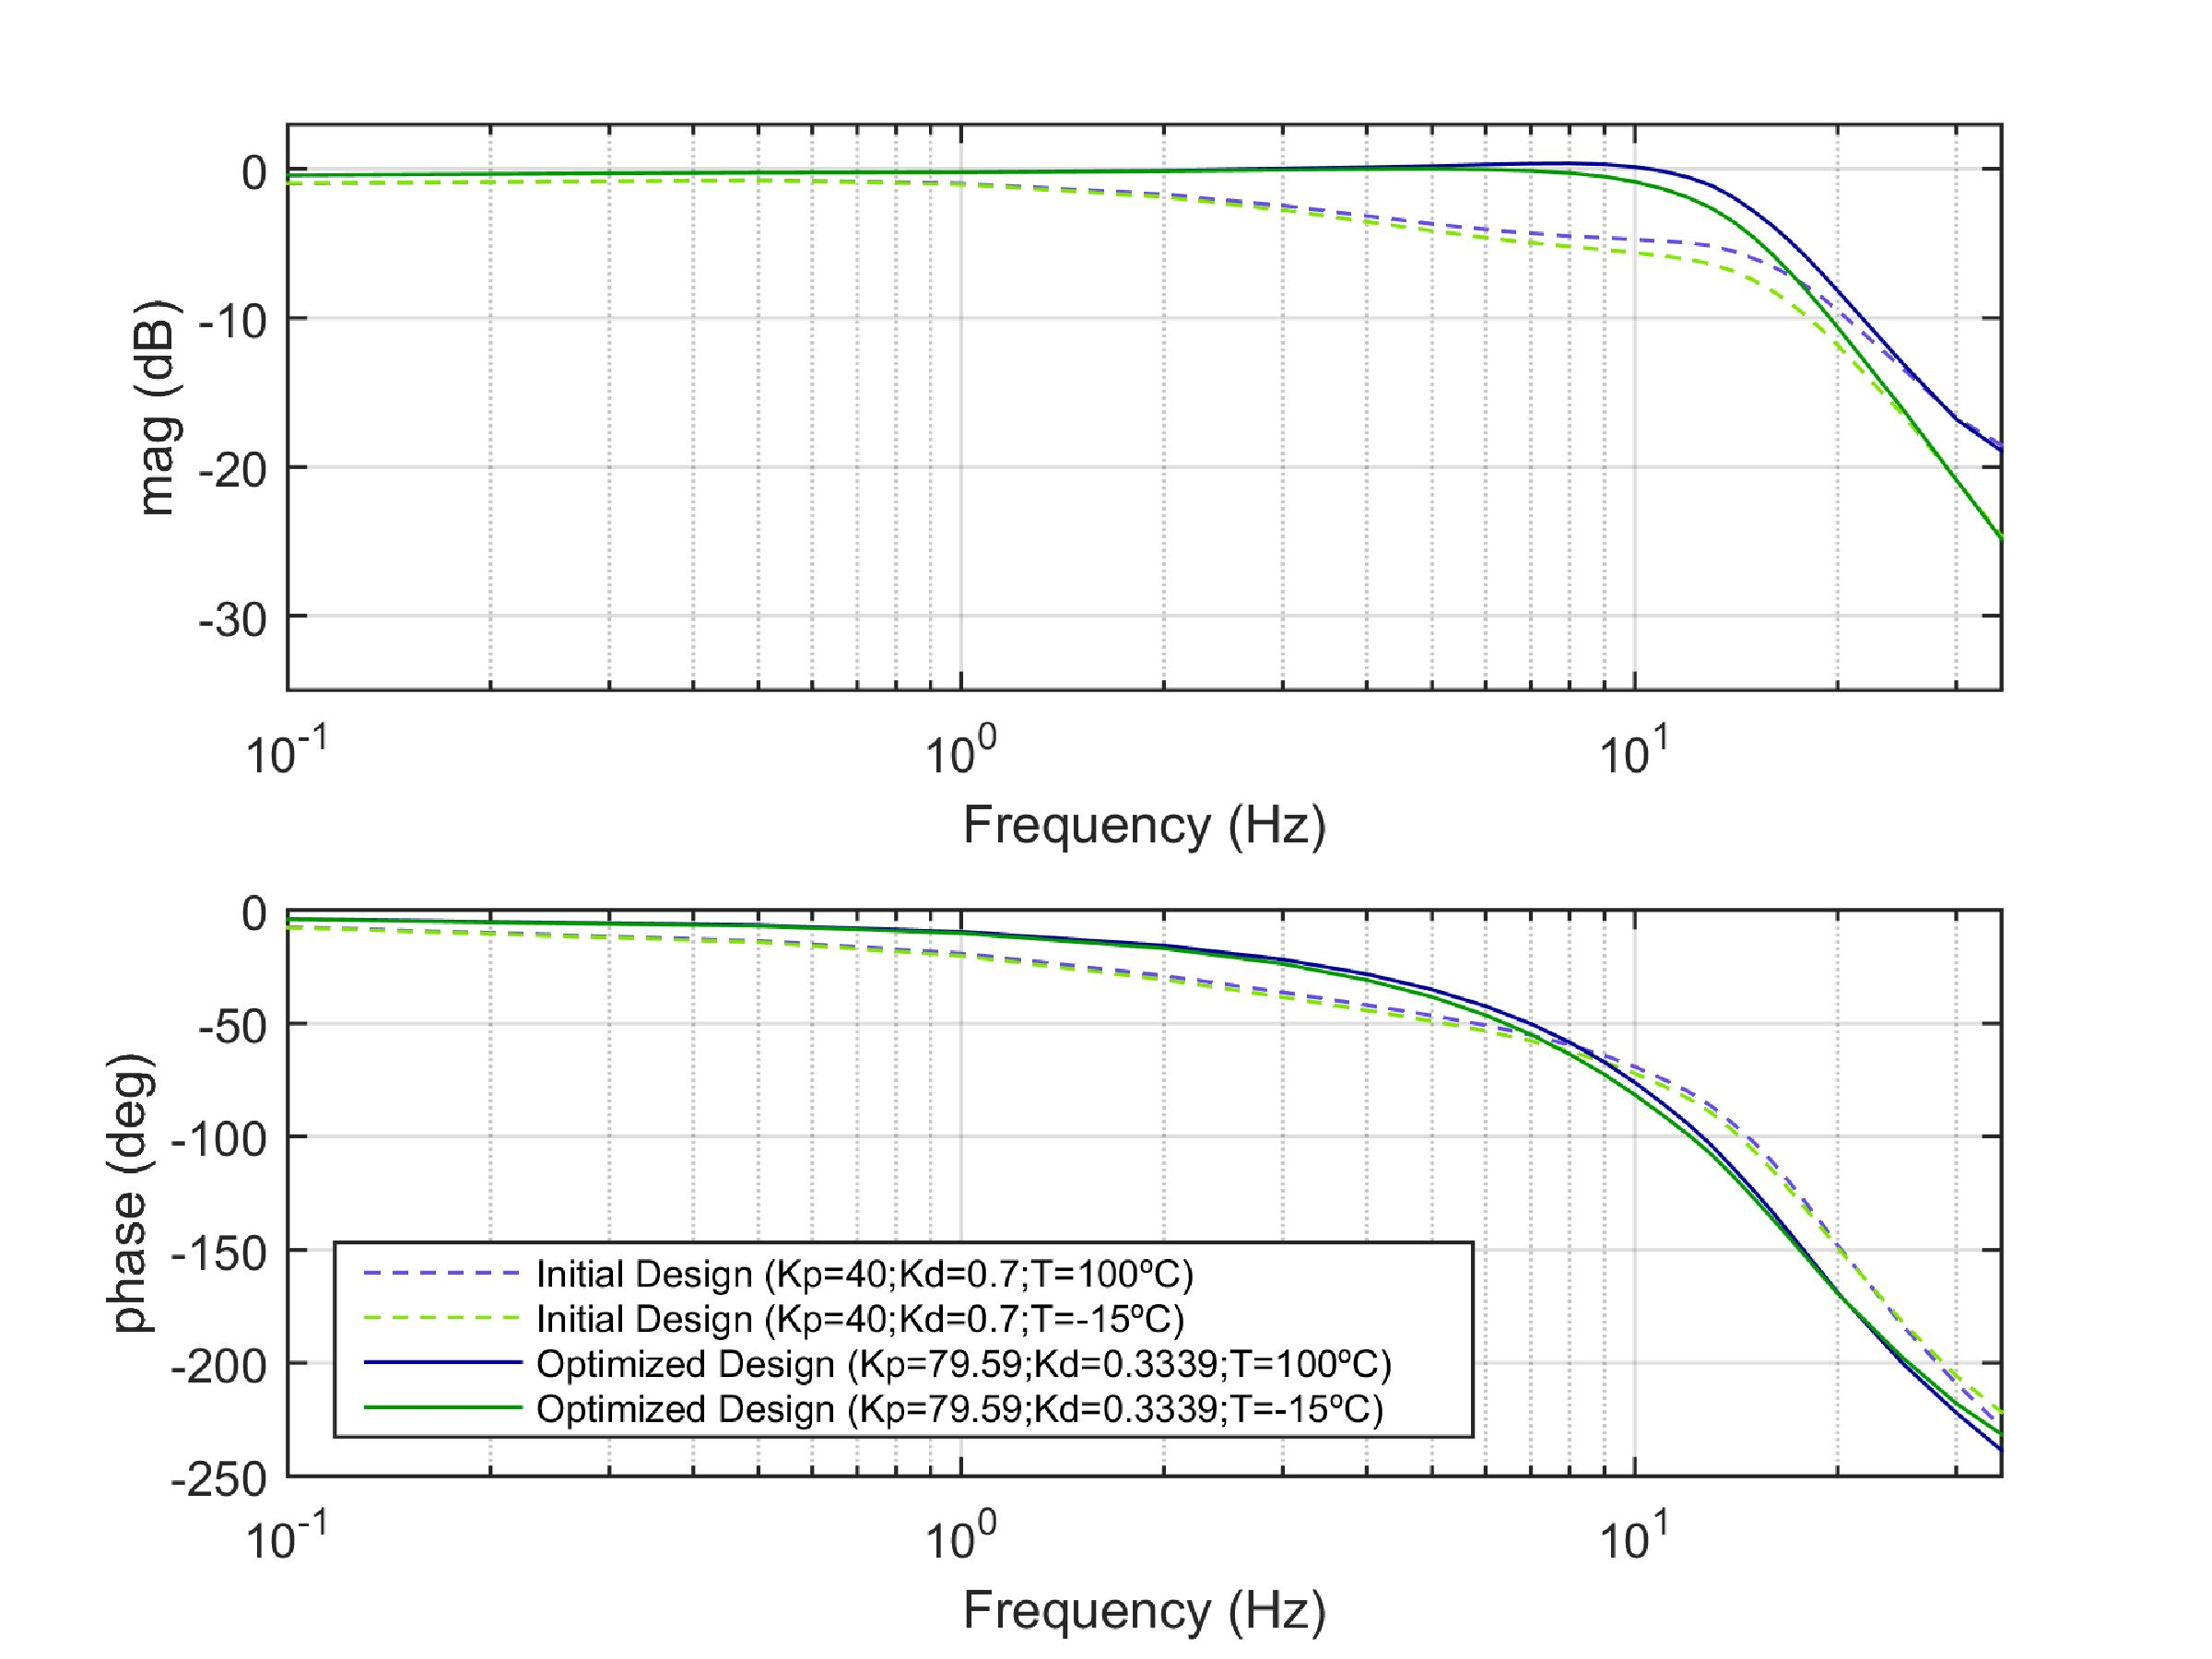
\includegraphics[width=0.9\textwidth]{Figuras/5.OptimizationResults/5-1-3-PD-FrequencyResponseComparison.jpg}}
	\caption{Frequency Response Baseline for the PD Controller.}
	\label{fig:5_1_3_PD_FreqResp}
\end{figure}

The closed-loop frequency response comparison is presented in Figure \ref{fig:5_1_3_PD_FreqResp} and the performance requirements are also shown in Table \ref{table:5_1_3_PD_PerfTable}. The closed-loop gain allowance was reduced and was just below requirement and the closed-loop phase allowance went from infinite to 99.2$°$. The magnitude response surpassed 0 dB and peaked at 0.38 dB, just below the 0.5dB requirement and the bandwidth increased considerably.

\begin{table}[H]
	\captionof{table}{Requirement Compliance for PD Controller}
	\label{table:5_1_3_PD_PerfTable}
	\centering
	\resizebox{14cm}{!} {
		\begin{tabular}{|l|c|c|c|c|}
			\hline
			Design Parameter & Requirement & Baseline & Optimized Controller & Difference (\%) \\ \hline
			Settling Time (ms) & $< 1100 $ & $992$ & $895$ & $-9.8$ \\ \hline
			Steady State Error ($\%$) & $< 1$ & $0.27$ & $0.14$ & $-48.1$ \\ \hline
			Overshoot ($\%$) & $< 10 $  & $0.0$ & $0.0$ & $N/A$ \\ \hline
			Minimum Average Rate ($°/s$) & $> 32$ & $34.32$ & $34.62$ & $0.9$ \\ \hline
			Maximum Average Rate ($°/s$) & $< 36$ & $34.32$ & $34.62$ & $0.9$ \\ \hline
			Closed-Loop Gain Allowance (dB) & $ \geq 10 $ & $13.00$ & $9.90$ & $-23.8$ \\ \hline
			Closed-Loop Phase Allowance ($°$) & $ \geq 45$ & $inf$ & $99.20$ & $N/A$ \\ \hline
			Closed-Loop Maximum Peak (dB) & $ < 0.5$ & $-0.74$ & $0.38$ & $151.4$ \\ \hline
			Closed-Loop Initial Magnitude (dB) & $None$ & $-0.99$ & $-0.41$ & $58.6$ \\ \hline
			Closed-Loop Bandwidth (Hz) & $None$ & $5.83$ & $15.59$ & $167.4$ \\ \hline
	\end{tabular}}
\end{table}

\subsection{Proportional  Integral Derivative Controller (PID)}

The proportional integral derivative controller optimization execution time was 16.4 hours and required 20 iterations, as per Table \ref{table:5_1_4_PIDContExecution}. Also, the optimization yielded a proportional gain of 76.05, integral gain of 3.285-9 and a derivative gain of 0.4318. These values were evaluated separately by \citeonline{Ballesteros} but were not considered together as a PID design.

\begin{table}[H]
	\captionof{table}{PID Controller Optimization Execution Results}
	\label{table:5_1_4_PIDContExecution}
	\centering
	\resizebox{7cm}{!} {
		\begin{tabular}{|l|c|}
			\hline
			Optimized Proportional Gain & 76.05 \\ \hline
			Optimized Integral Gain & 3.285e-9 \\ \hline
			Optimized Derivative Gain & 0.4318 \\ \hline
			Optimization Execution Time (h) & 16.4 \\ \hline
			Number of Iterations & 20 \\ \hline		
			Number of Obj. Function Evaluations & 111 \\ \hline		
	\end{tabular}}
\end{table}

The  dynamic stiffness response for each PID design is shown in Figure \ref{fig:5_1_4_PID_DynStif}. Similarly to the PD controller, increase in dynamic stiffness was observed in frequencies below 3Hz and also a fair reduction was observed in higher frequencies.

\begin{figure}[H]
	\centering
	\centerline{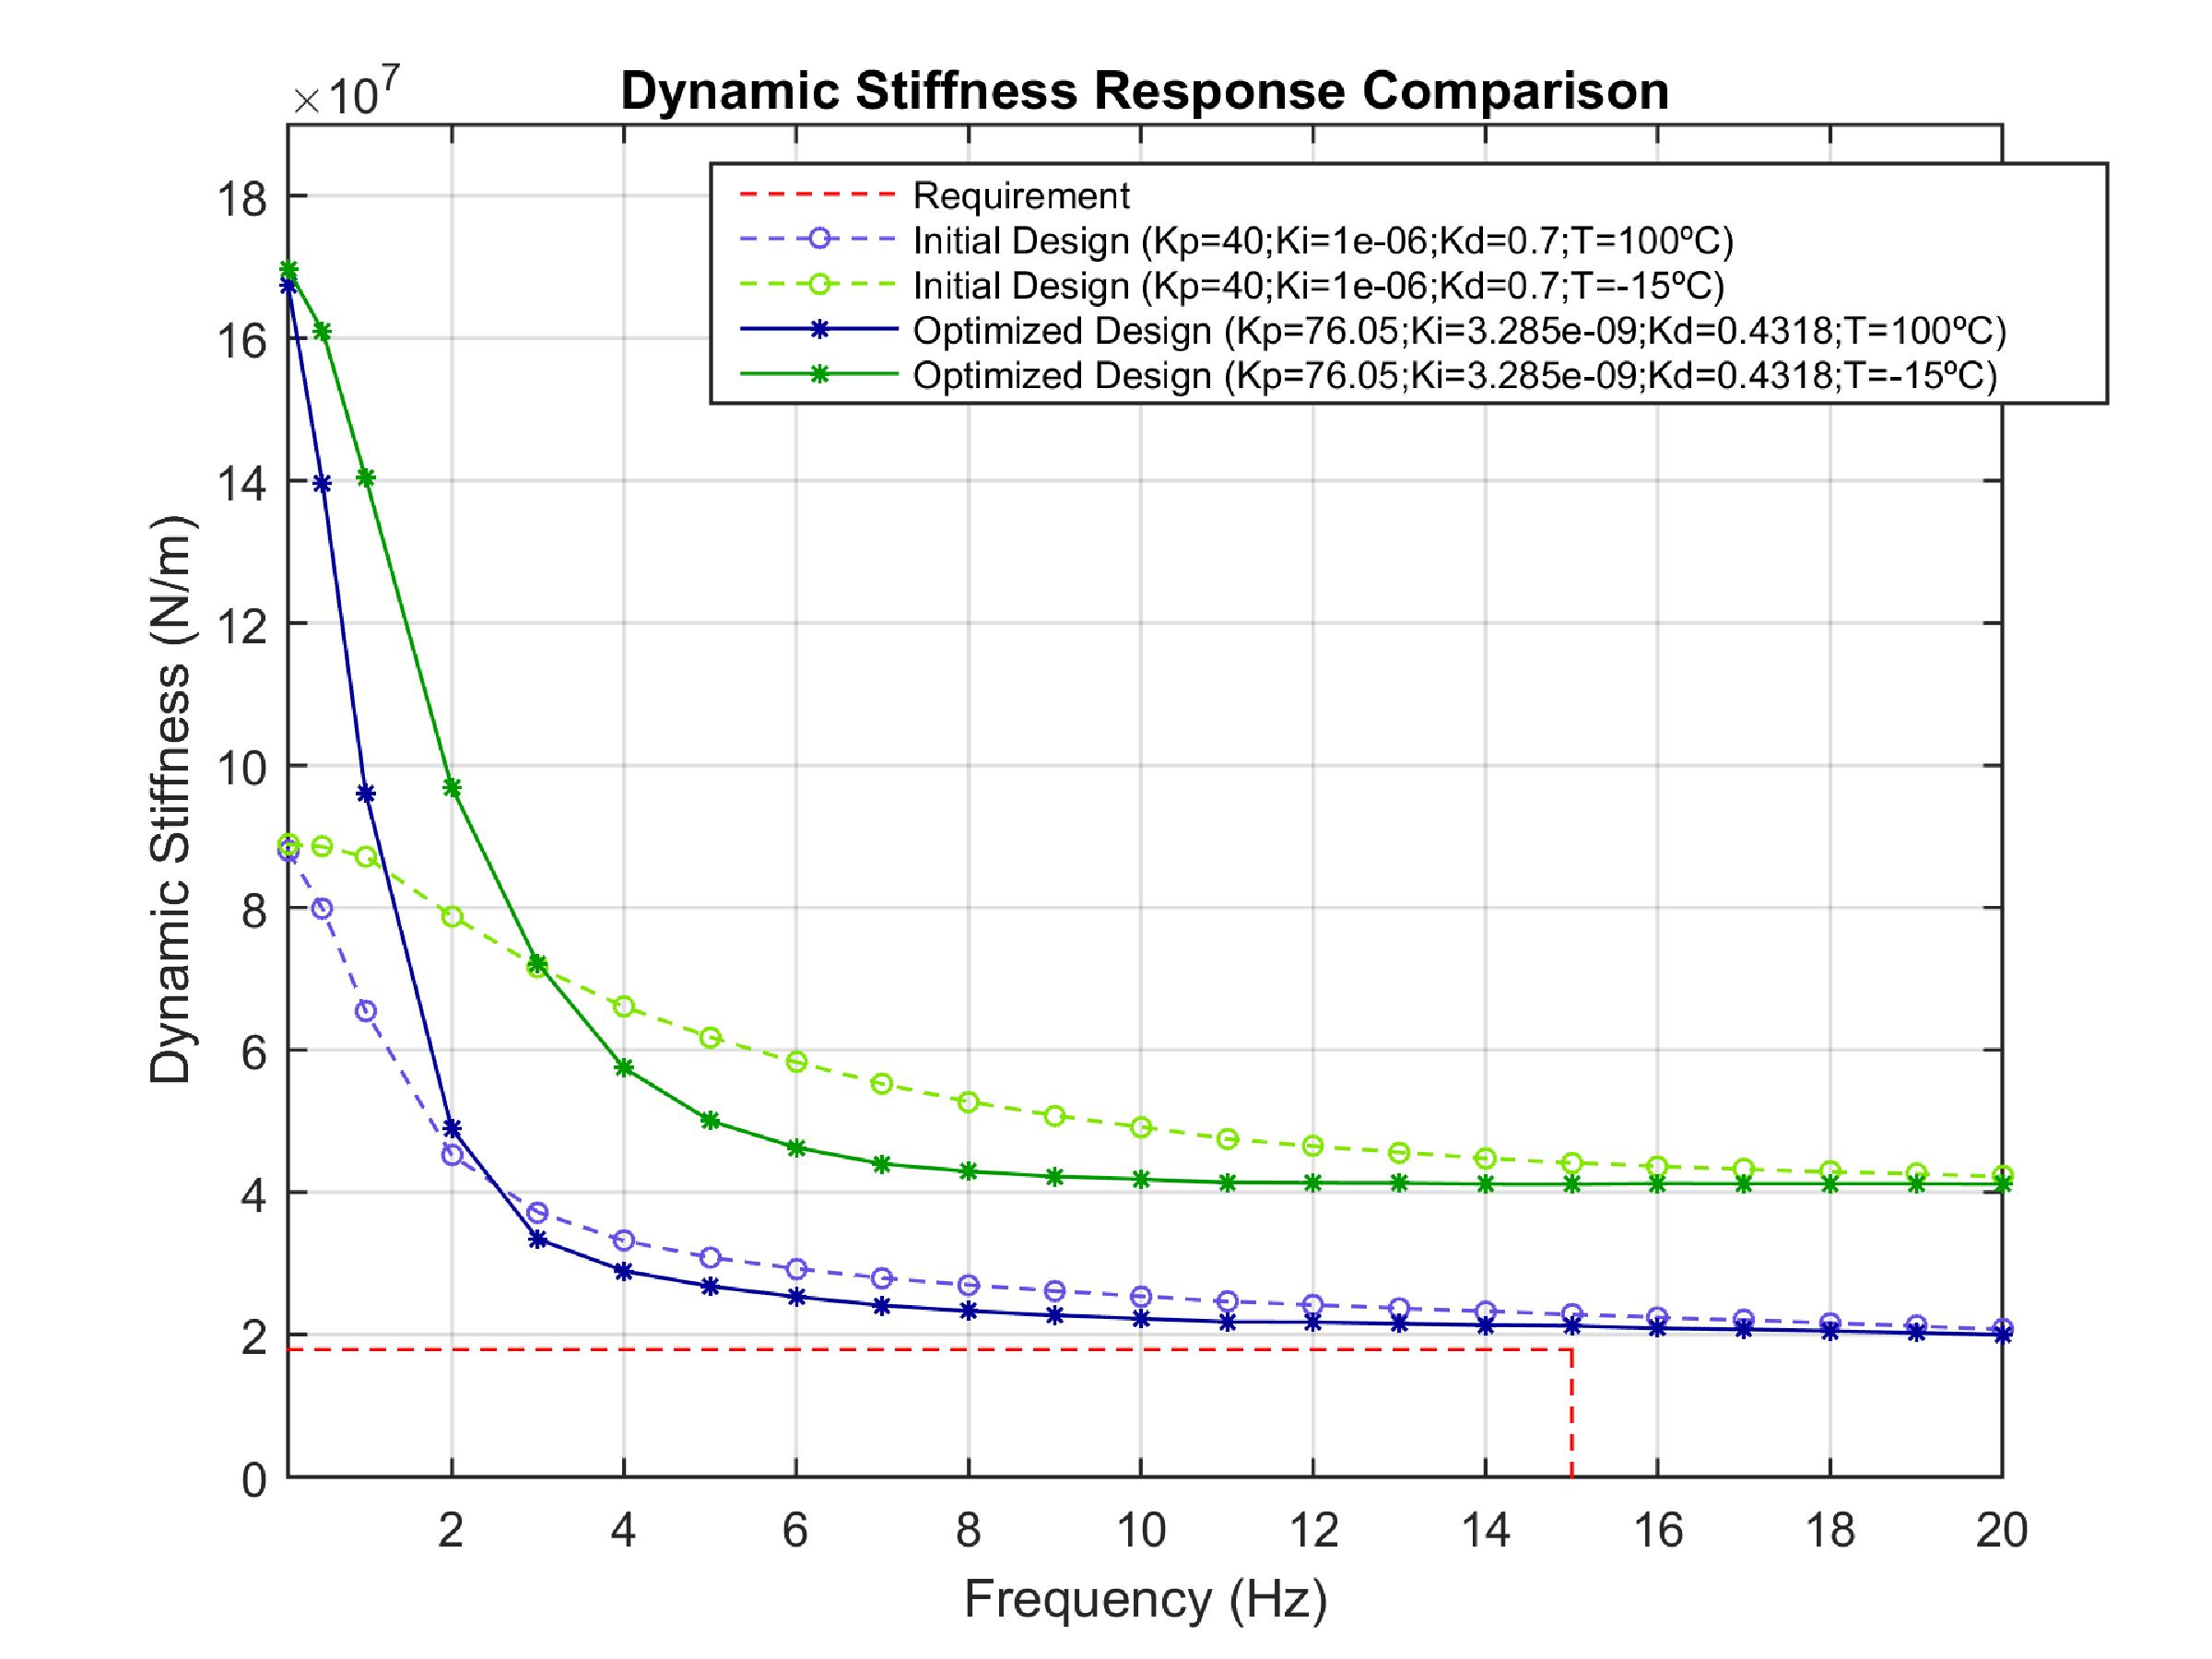
\includegraphics[width=0.9\textwidth]{Figuras/5.OptimizationResults/5-1-4-PID-DynamicStiffnessComparison.jpg}}
	\caption{Dynamic Stiffness Optimization Result for the PID Controller.}
	\label{fig:5_1_4_PID_DynStif}
\end{figure}

Table \ref{table:5_1_4_PID_CostFunctionTable} show the partial values of the cost function for each frequency evaluated by the dynamic stiffness test. The lower frequencies values are considerably larger since stiffness increase occurred in this range. 

\begin{table}[H]
	\captionof{table}{PID Controller Final Solution Cost Function for Each Evaluated Frequency}
	\label{table:5_1_4_PID_CostFunctionTable}
	\centering
	\resizebox{14cm}{!} {
		\begin{tabular}{|c|c|c|c|c|c|}
			\hline
			Frequency (Hz) & $J_i$ & Frequency (Hz) & $J_i$ & Frequency (Hz) & $J_i$ \\ \hline
			$0.1$ & $1.5e+08$ & $5$ & $8.9e+06$ & $11$ & $3.89e+06$ \\ \hline
			$0.5$ & $1.22e+08$ & $6$ & $7.42e+06$ & $12$ & $3.87e+06$ \\ \hline
			$1$ & $7.82e+07$ & $7$ & $6.2e+06$ & $13$ & $3.66e+06$ \\ \hline
			$2$ & $3.1e+07$ & $8$ & $5.43e+06$ & $14$ & $3.44e+06$ \\ \hline
			$3$ & $1.55e+07$ & $9$ & $4.81e+06$ & $15$ & $3.33e+06$ \\ \hline
			$4$ & $1.1e+07$ & $10$ & $4.36e+06$ & $0$ & $0$ \\ \hline
	\end{tabular}}
\end{table}

The time response comparison is presented in Figure \ref{fig:5_1_4_PID_TimeResp} and the performance requirements are shown in Table \ref{table:5_1_4_PID_PerfTable}. The settling time was reduced by 94ms and the steady state error decreased by almost 50\%. 

\begin{figure}[H]
	\centering
	\centerline{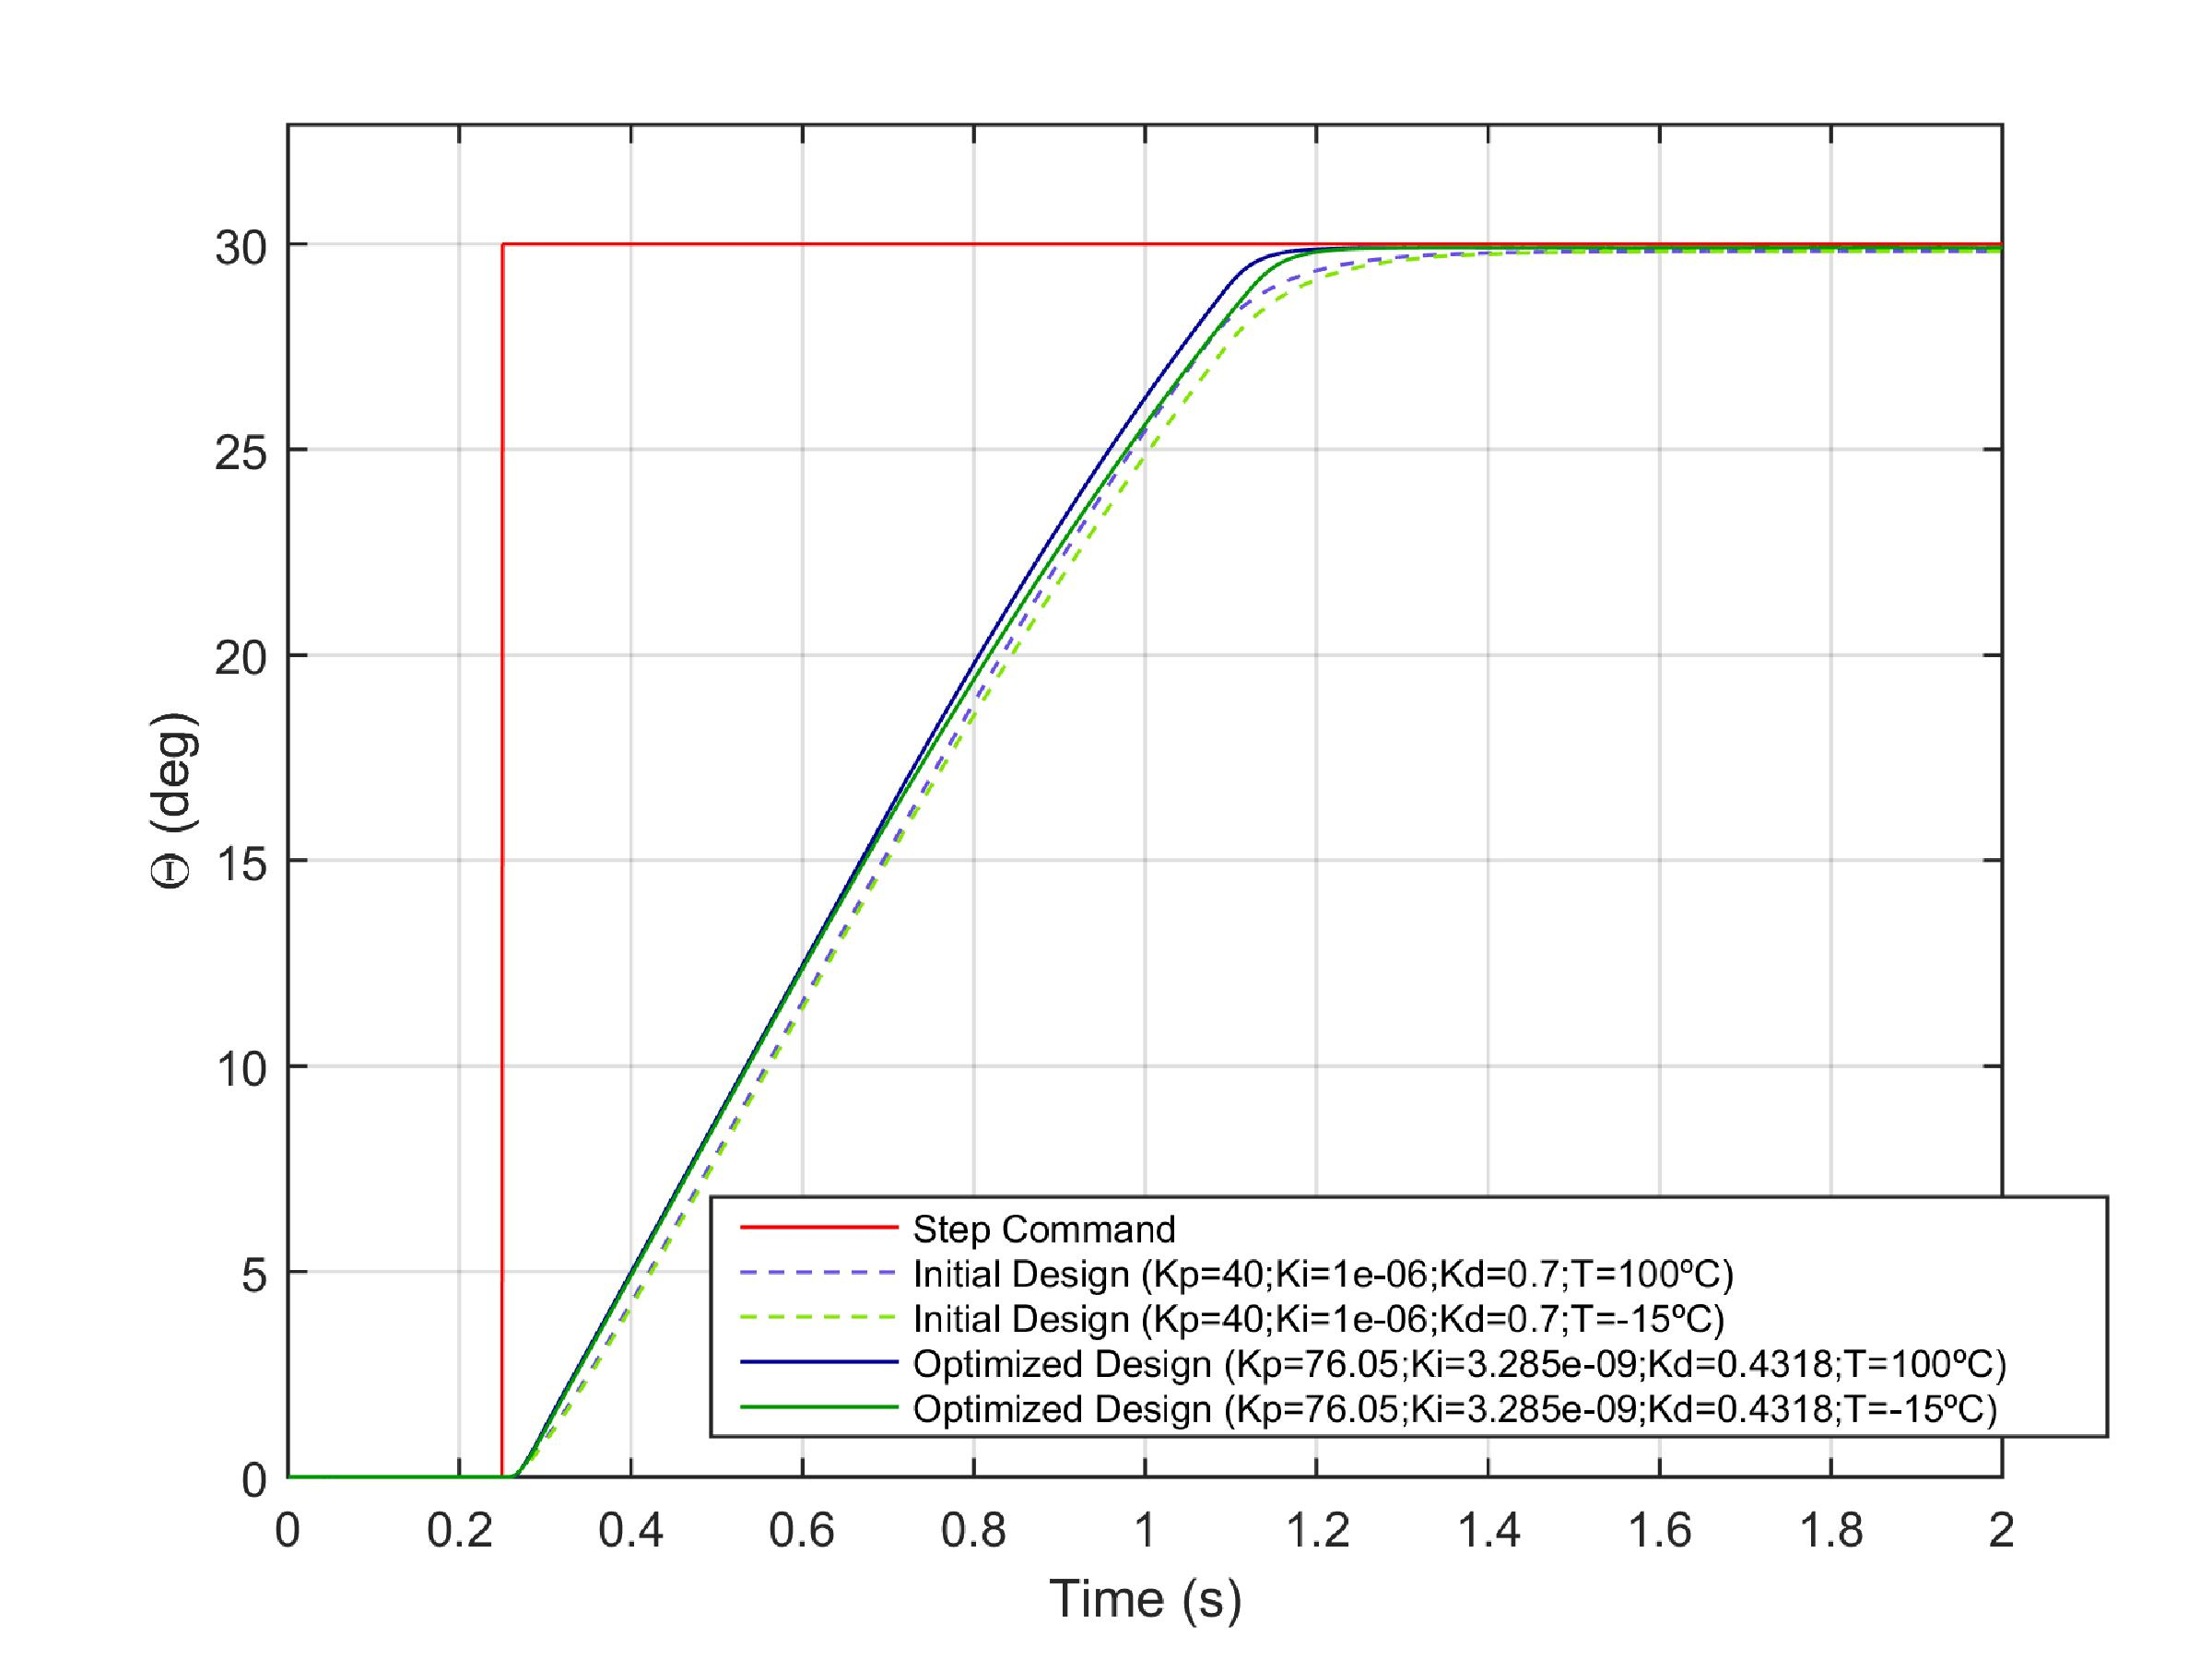
\includegraphics[width=0.9\textwidth]{Figuras/5.OptimizationResults/5-1-4-PID-TimeResponseComparison.jpg}}
	\caption{Time Response Optimization Result for the PID Controller.}
	\label{fig:5_1_4_PID_TimeResp}
\end{figure}

The closed-loop frequency response comparison is presented in Figure \ref{fig:5_1_4_PID_FreqResp} and the performance requirements are also shown in Table \ref{table:5_1_4_PID_PerfTable}. The closed-loop gain allowance was reduced and was slightly lower than requirement and the closed-loop phase allowance remained infinite. 

\begin{figure}[H]
	\centering
	\centerline{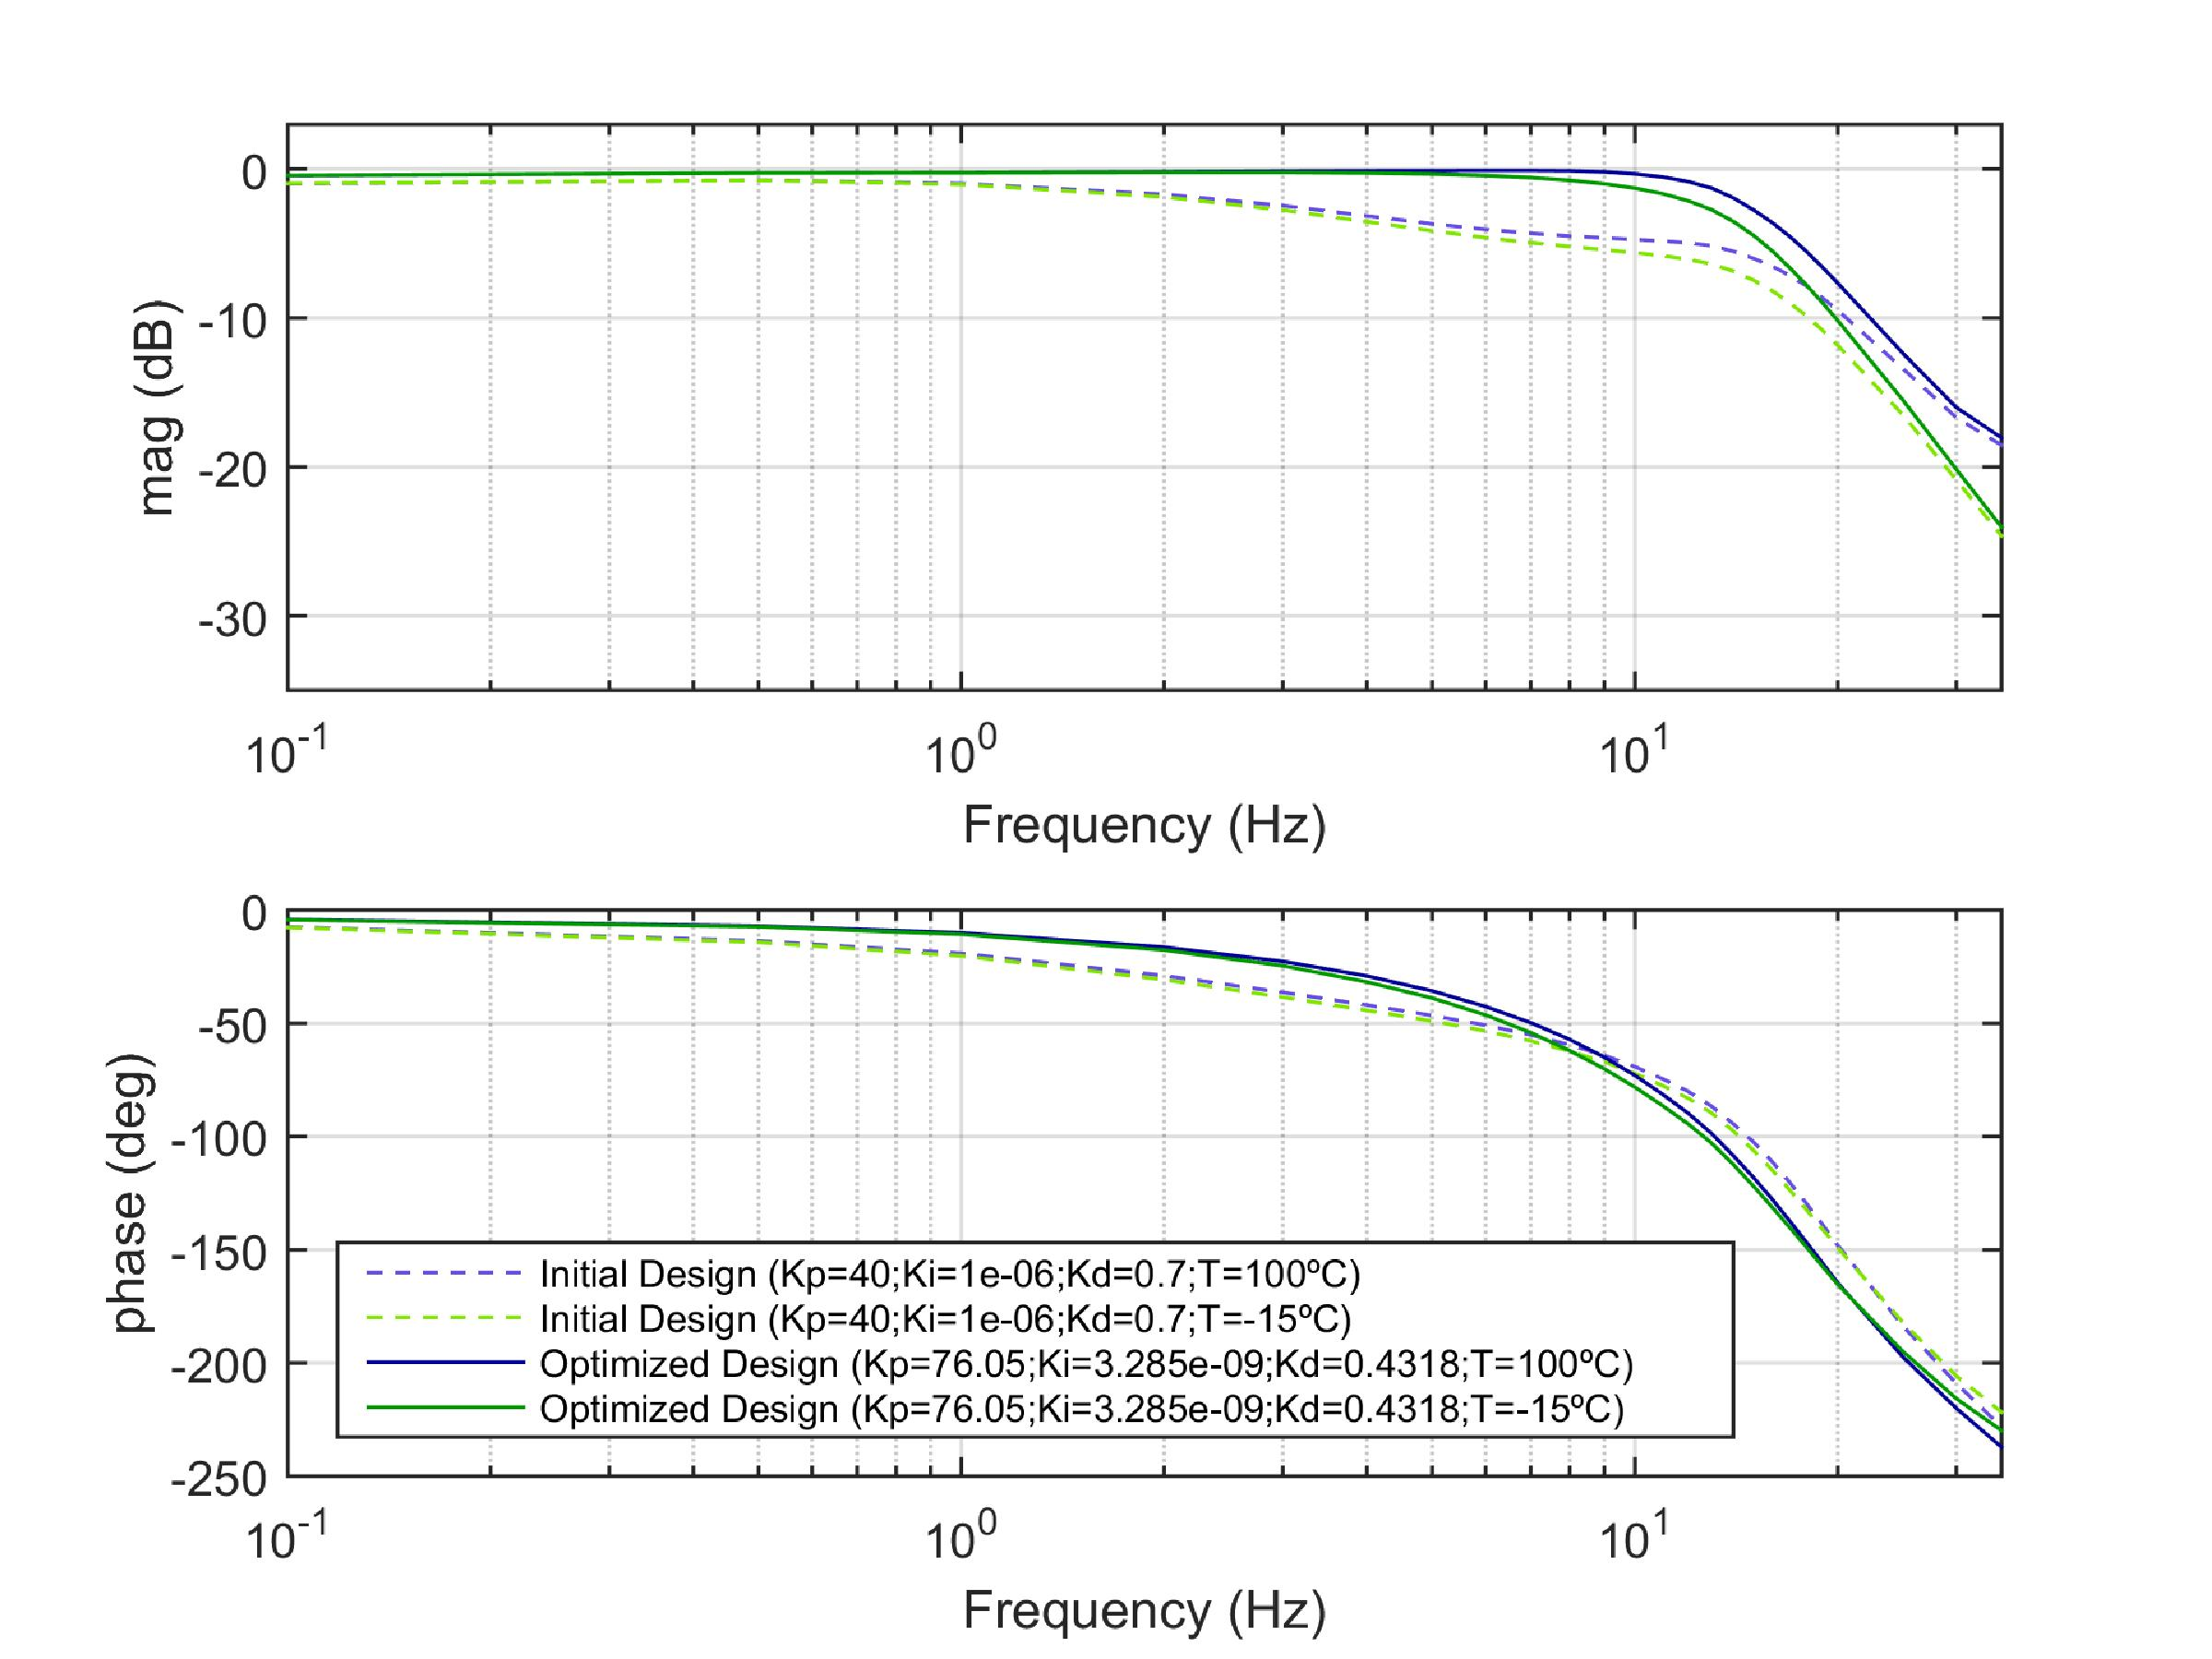
\includegraphics[width=0.9\textwidth]{Figuras/5.OptimizationResults/5-1-4-PID-FrequencyResponseComparison.jpg}}
	\caption{Frequency Response Baseline for the PID Controller.}
	\label{fig:5_1_4_PID_FreqResp}
\end{figure}

\begin{table}[H]
	\captionof{table}{Requirement Compliance for PID Controller}
	\label{table:5_1_4_PID_PerfTable}
	\centering
	\resizebox{14cm}{!} {
		\begin{tabular}{|l|c|c|c|c|}
			\hline
			Design Parameter & Requirement & Baseline & Optimized Controller & Difference (\%) \\ \hline
			Settling Time (ms) & $< 1100 $ & $992$ & $898$ & $-9.5.$ \\ \hline
			Steady State Error ($\%$) & $< 1$ & $0.27$ & $0.14$ & $-48.1$ \\ \hline
			Overshoot ($\%$) & $< 10 $  & $0.0$ & $0.0$ & $N/A$ \\ \hline
			Minimum Average Rate ($°/s$) & $> 32$ & $34.32$ & $34.61$ & $0.8$ \\ \hline
			Maximum Average Rate ($°/s$) & $< 36$ & $34.32$ & $34.61$ & $0.8$ \\ \hline
			Closed-Loop Gain Allowance (dB) & $ \geq 10 $ & $13.00$ & $9.87$ & $-24.1$ \\ \hline
			Closed-Loop Phase Allowance ($°$) & $ \geq 45$ & $inf$ & $inf$ & $N/A$ \\ \hline
			Closed-Loop Maximum Peak (dB) & $ < 0.5$ & $-0.74$ & $-0.10$ & $86.5$ \\ \hline
			Closed-Loop Initial Magnitude (dB) & $None$ & $-0.99$ & $-0.44$ & $55.6$ \\ \hline
			Closed-Loop Bandwidth (Hz) & $None$ & $5.83$ & $15.8$ & $171.0$ \\ \hline
	\end{tabular}}
\end{table}

The results obtained for P and PI controllers are very similar what is coherent with previous findings which showed that integral gain does not influence dynamic stiffness. The same occurred between PD and PID controllers results that were also fairly similar.

Optimization for all controllers yielded improvement in overall dynamic stiffness as expected, however, a tendency for increases in lower frequencies is clear. This can be explained by the fact that the control loop has a high influence in lower frequency dynamic stiffness because is where it can respond faster to external disturbances.

These results also show a relationship between time response performance improvement (mainly settling time and steady state error) and dynamic stiffness reduction in high frequencies. Therefore, this suggests that to increase dynamic stiffness a reduction in time domain performance would be required. 

A deterioration of frequency domain performance was observed for all controllers, including a requirement violation for proportional controller (closed-loop peak magnitude) and for PD and PID controllers (closed-loop gain allowance). These findings suggest that improvement in time domain performance also jeopardize frequency domain parameters.

In summary, this section has shown that the developed algorithm delivers overall increase in dynamic stiffness. However, its cost function considers improvements in both low and high frequencies equally what has led to dynamic stiffness improvements only in low frequencies and inferior values at the infinite frequency. 

Hence, the solutions yielded by the optimization diminish flutter suppression characteristics when compared to the initial solutions. This result did not satisfy the main goal of the optimization and, therefore, a change in the cost function was necessary. The next section presents a new set of results obtained by the optimization considering a frequency weighted cost function.

\section{Classic Controllers and Frequency Weighted Cost Function}

This section presents the results obtained through the optimization considering a more complex cost function, described in Equation \ref{eq:4_4_3_ContrainedWeightedEquation}. The initial solutions in this case were the same used to obtain the previous results and are shown in Table \ref{table:5_1_InitSolutTable}.

\subsection{Proportional Controller (P)}

The results obtained with the weighted cost function for the proportional controller are presented in this section. As shown in table \ref{table:5_2_1_PContExecution}, the execution time of the optimization was 2.5 hours and 7 iterations were performed until stopping criteria was reached. Also, the proportional gain after optimization is 24.74. This value is in the range evaluated by \citeonline{Ballesteros} and therefore similar behavior as the one observed by the author is expected. 

\begin{table}[H]
	\captionof{table}{P Controller Optimization Execution Results}
	\label{table:5_2_1_PContExecution}
	\centering
	\resizebox{7cm}{!} {
		\begin{tabular}{|l|c|}
			\hline
			Optimized Proportional Gain & 24.74 \\ \hline
			Optimization Execution Time (h) & 6.4 \\ \hline
			Number of Iterations & 4 \\ \hline	
			Number of Obj. Function Evaluations & 42 \\ \hline		
	\end{tabular}}
\end{table}

The  dynamic stiffness response for each design is shown in Figure \ref{fig:5_2_1_P_DynStif}. Despite a decrease in lower frequencies, an increase in dynamic stiffness is observed in all frequencies above 4Hz, including the infinite frequency. 

The result is coherent with previous studies findings that for proportional controllers the dynamic stiffness at the infinite frequency are higher when the gain is smaller \cite{Ballesteros}. Also, comparing Figures \ref{fig:5_2_1_P_DynStif} and \ref{fig:5_1_1_P_DynStif} is possible to note the impact of changing the cost function on the final optimization result.

\begin{figure}[H]
	\centering
	\centerline{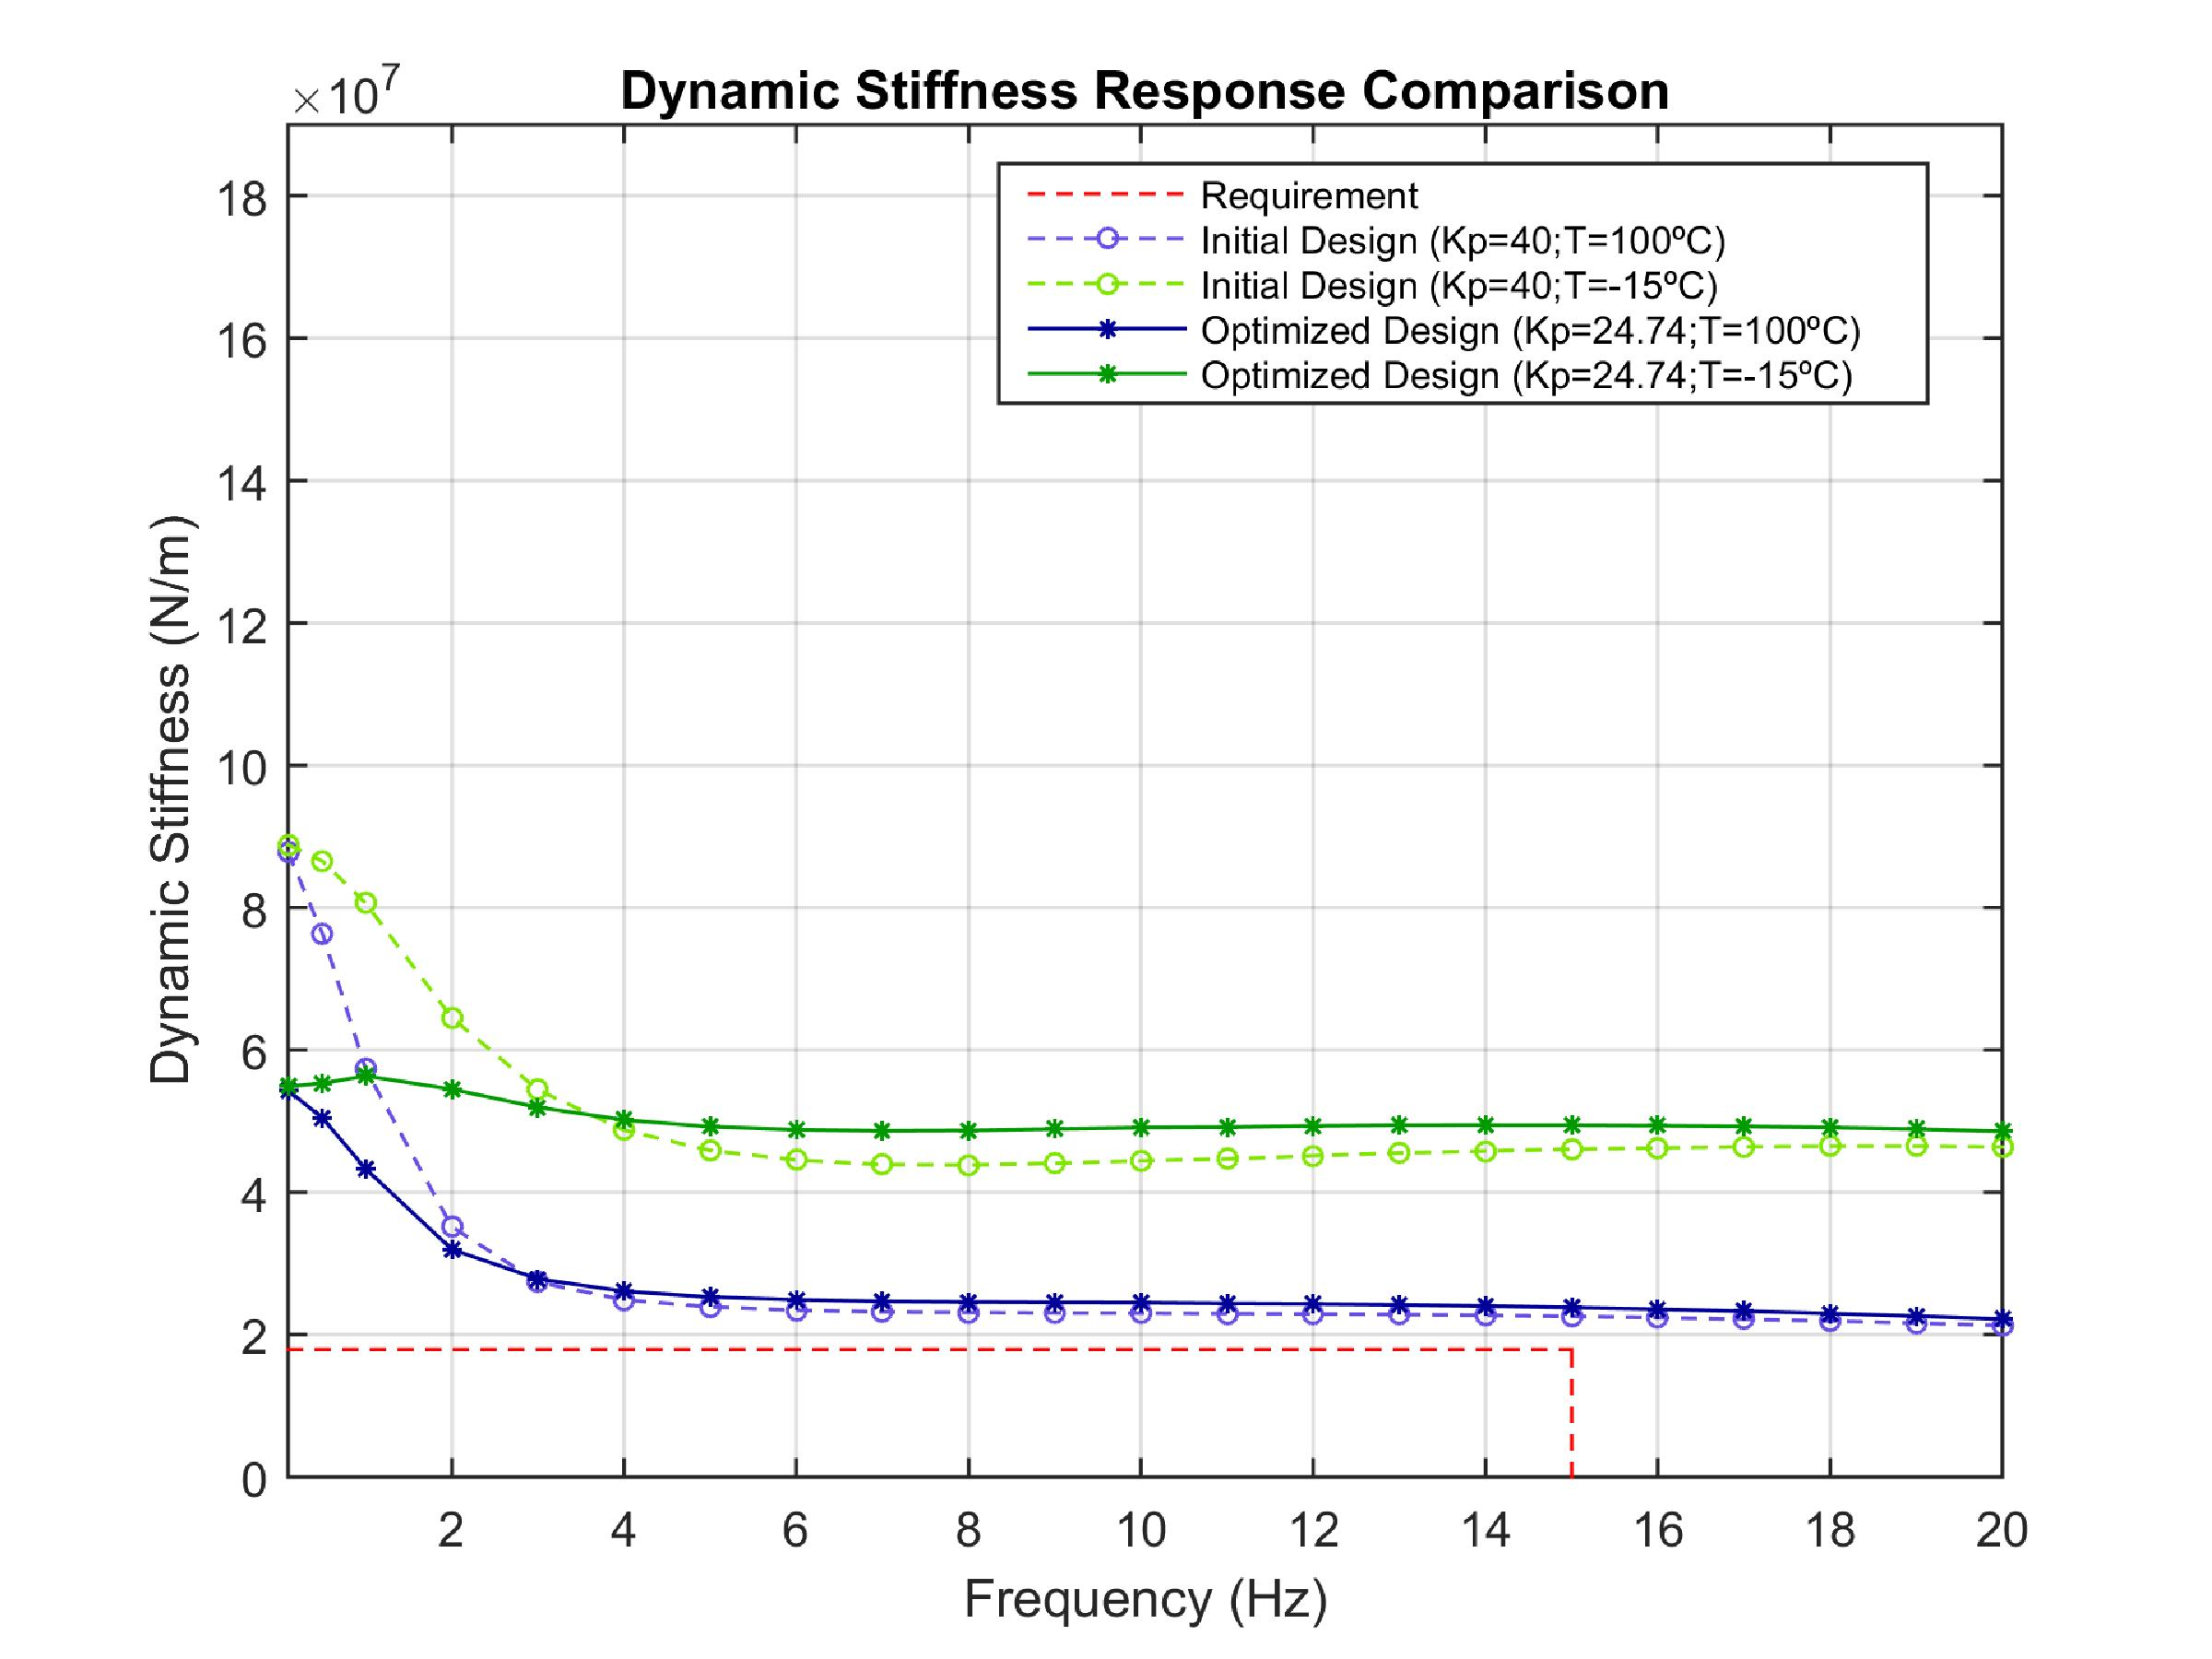
\includegraphics[width=0.9\textwidth]{Figuras/5.OptimizationResults/5-2-1-P-DynamicStiffnessComparison.jpg}}
	\caption{Dynamic Stiffness Comparison for Proportional Controller.}
	\label{fig:5_2_1_P_DynStif}
\end{figure}

Table \ref{table:5_2_1_P_CostFunctionTable} show the partial values of the cost function for each frequency evaluated by the dynamic stiffness test. The values at the lower frequencies are still larger than in higher frequencies but the difference is not as great as in Table \ref{table:5_1_1_P_CostFunctionTable}. This shows that even with smaller partial cost functions at 15Hz the algorithm preserved this solutions because of the high weight this partial has on the global cost function.

\begin{table}[H]
	\captionof{table}{P Controller Final Solution Cost Function for Each Evaluated Frequency}
	\label{table:5_2_1_P_CostFunctionTable}
	\centering
	\resizebox{14cm}{!} {
		\begin{tabular}{|c|c|c|c|c|c|}
			\hline
			Frequency (Hz) & $J_i$ & Frequency (Hz) & $J_i$ & Frequency (Hz) & $J_i$ \\ \hline
			$0.1$ & $1.51e+07$ & $5$ & $9.5e+06$ & $11$ & $8.25e+06$ \\ \hline
			$0.5$ & $1.56e+07$ & $6$ & $9.2e+06$ & $12$ & $8.05e+06$ \\ \hline
			$1$ & $1.65e+07$ & $7$ & $8.96e+06$ & $13$ & $7.81e+06$ \\ \hline
			$2$ & $1.29e+07$ & $8$ & $8.79e+06$ & $14$ & $7.53e+06$ \\ \hline
			$3$ & $1.1e+07$ & $9$ & $8.63e+06$ & $15$ & $7.2e+06$ \\ \hline
			$4$ & $1e+07$ & $10$ & $8.47e+06$ &  &  \\ \hline
	\end{tabular}}
\end{table}

The time response comparison is presented in Figure \ref{fig:5_2_1_P_TimeResp} and the performance requirements are shown in Table \ref{table:5_2_1_P_PerfTable}. The settling time increased by 142ms and was slightly higher than requirement. The steady state error increased approximately 60\% and the average rate of actuation slightly decreased. 

\begin{figure}[H]
	\centering
	\centerline{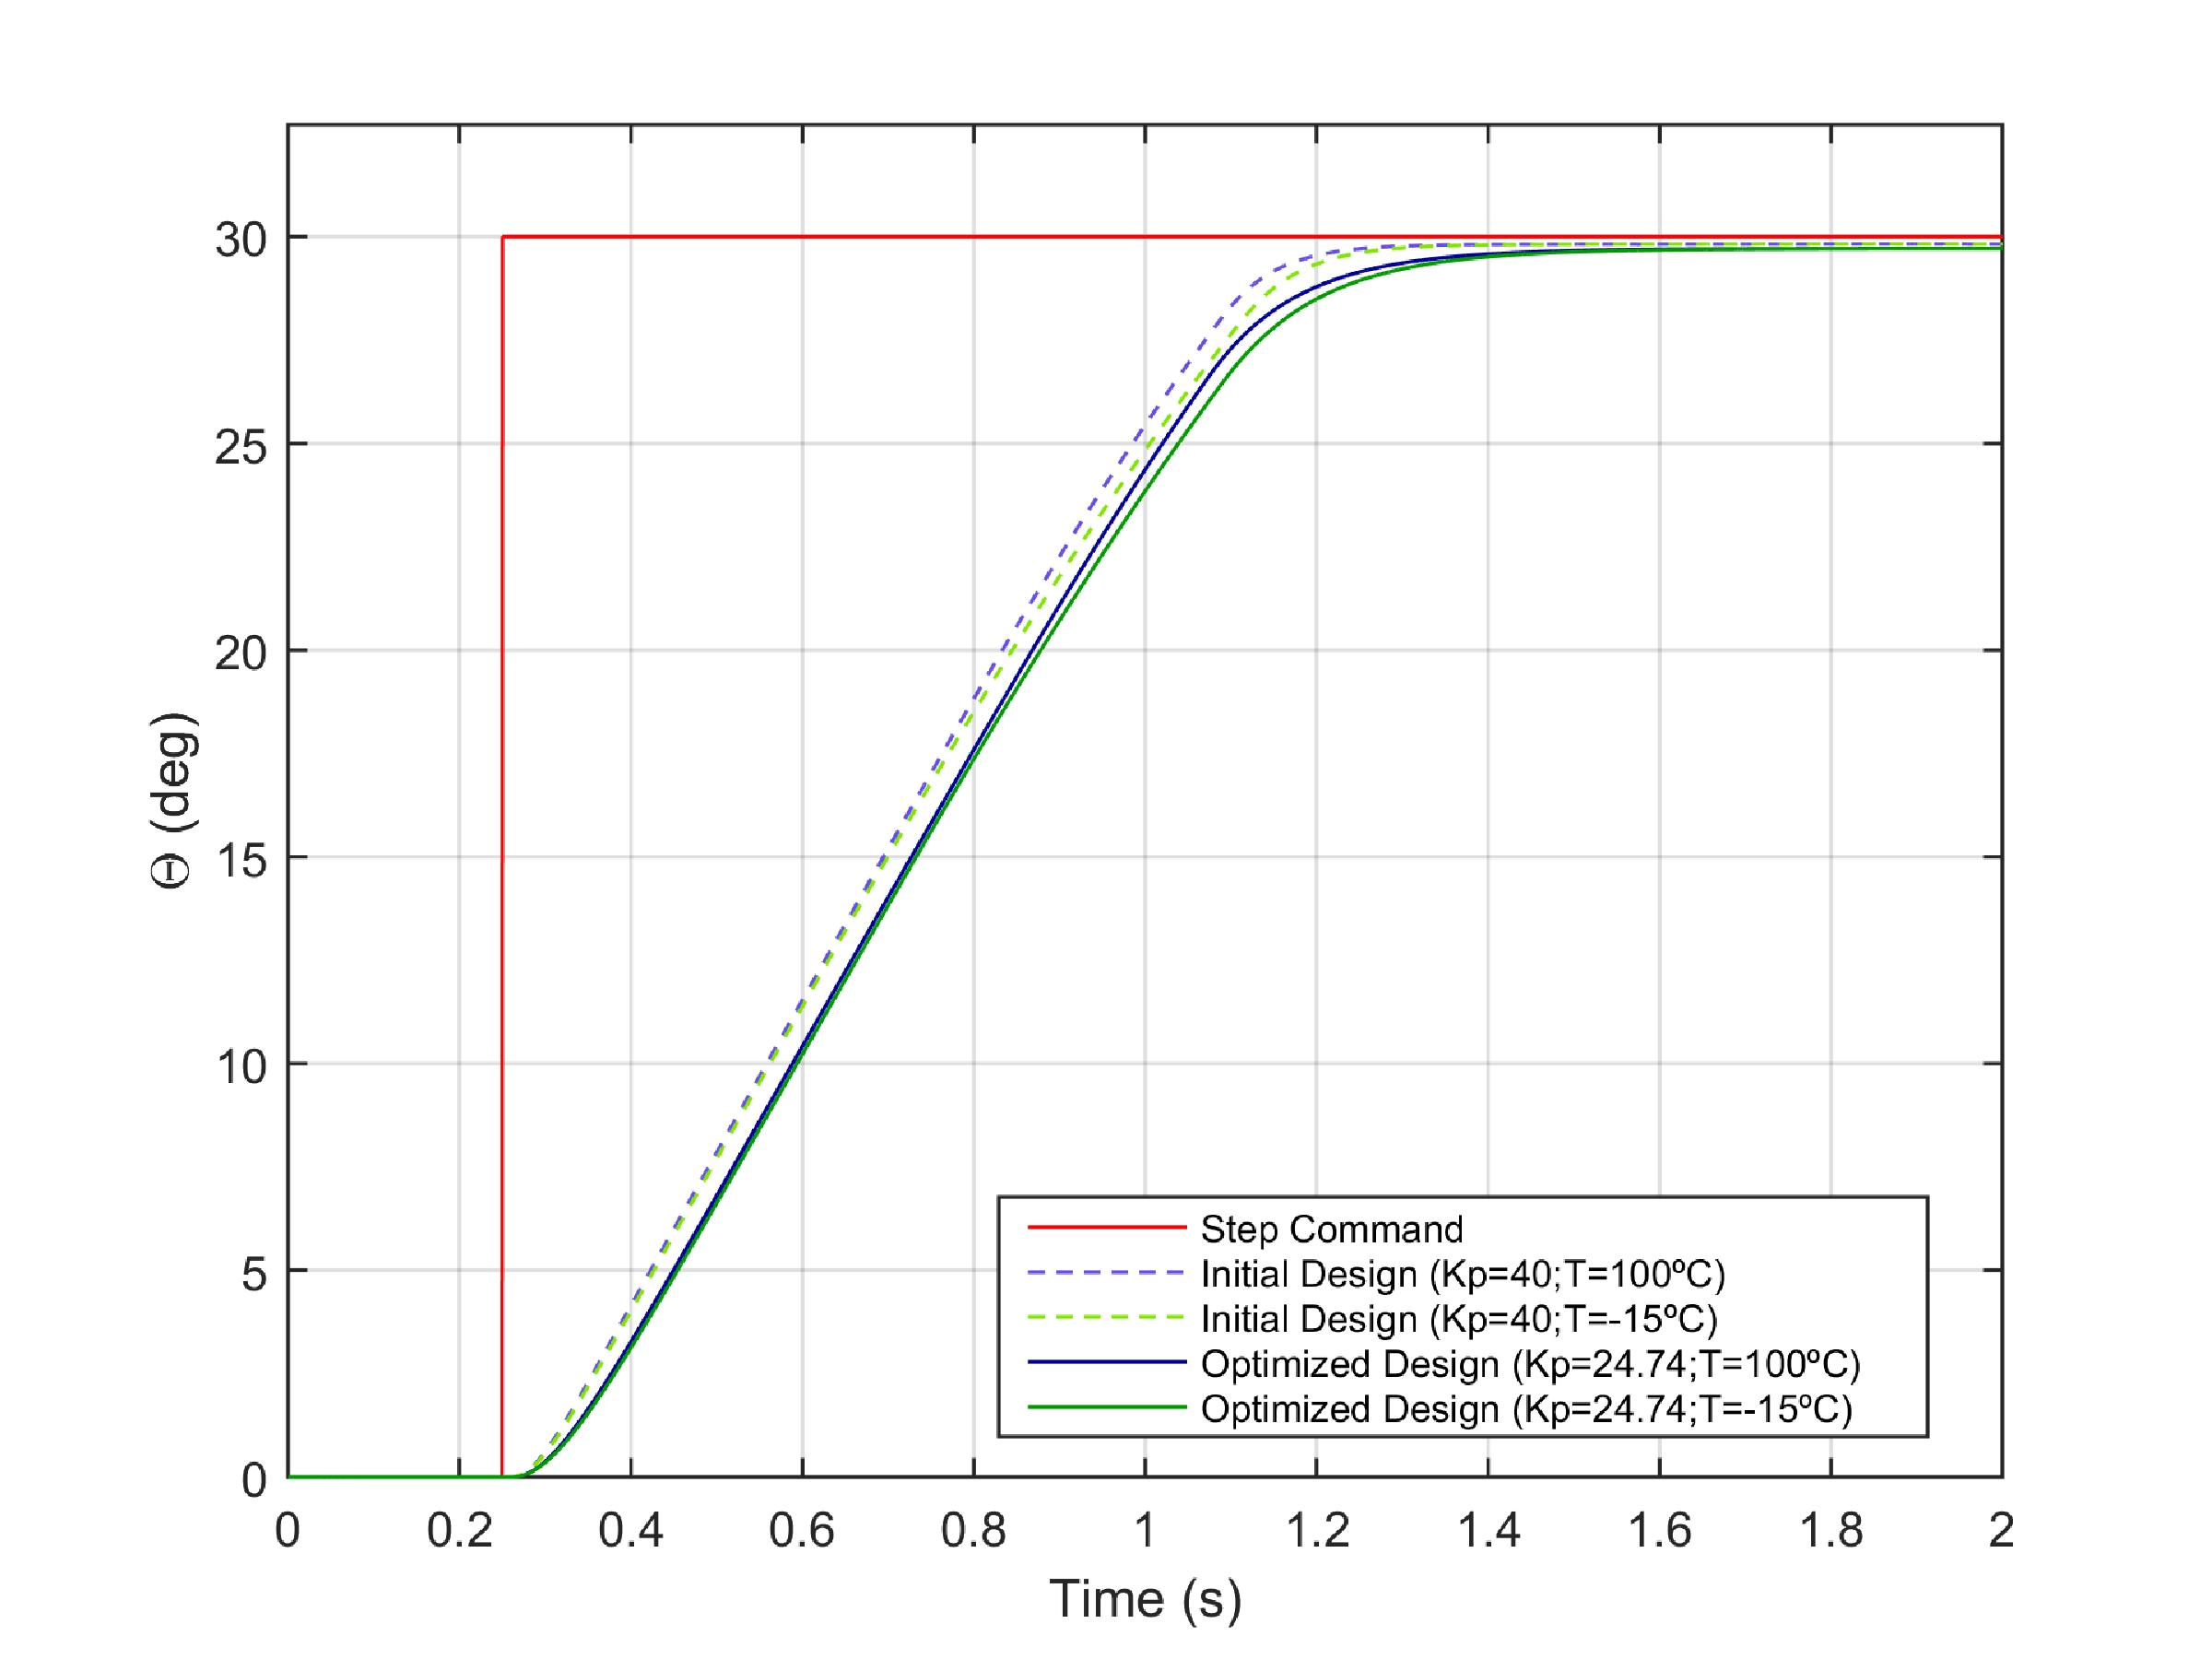
\includegraphics[width=0.9\textwidth]{Figuras/5.OptimizationResults/5-2-1-P-TimeResponseComparison.jpg}}
	\caption{Time Response Comparison for Proportional Controller.}
	\label{fig:5_2_1_P_TimeResp}
\end{figure}

\begin{figure}[H]
	\centering
	\centerline{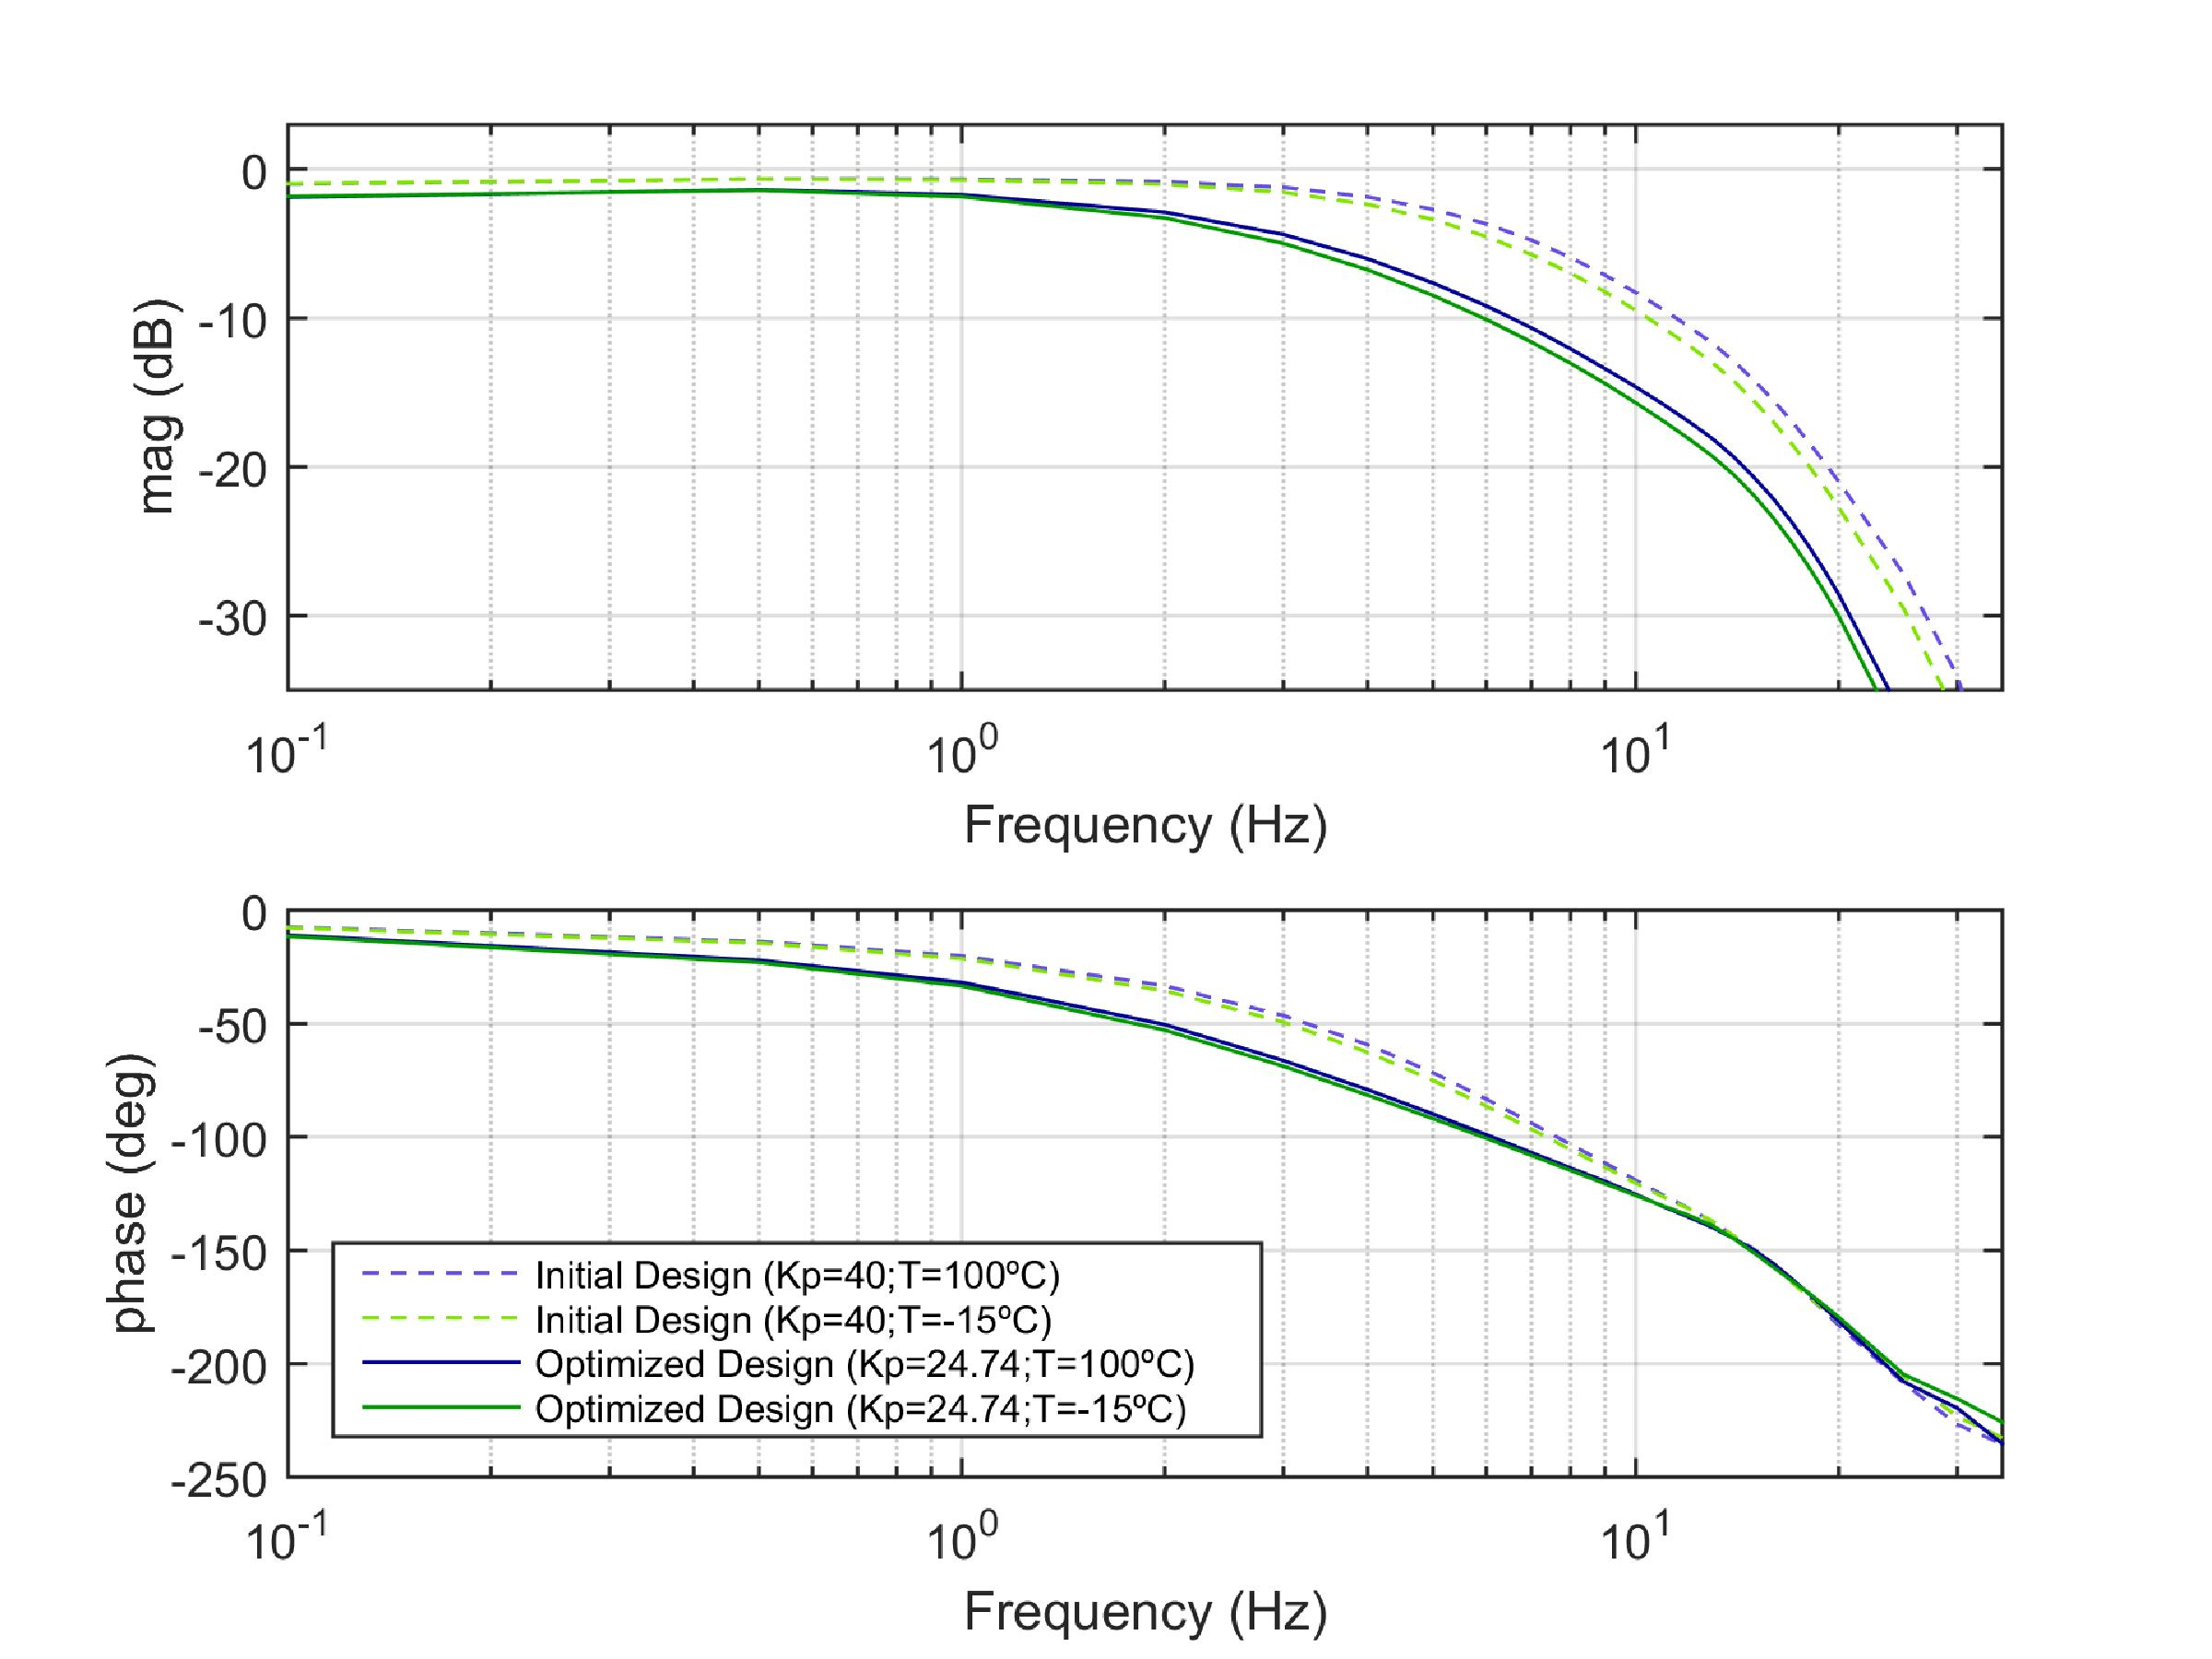
\includegraphics[width=0.9\textwidth]{Figuras/5.OptimizationResults/5-2-1-P-FrequencyResponseComparison.jpg}}
	\caption{Frequency Response Comparison for Proportional Controller.}
	\label{fig:5_2_1_P_FreqResp}
\end{figure}

The closed-loop frequency response comparison is presented in Figure \ref{fig:5_2_1_P_FreqResp} and the performance requirements are also shown in Table \ref{table:5_2_1_P_PerfTable}. The closed-loop gain allowance increased and the closed-loop phase allowance remained infinite.

Both frequency and time performances of the optimized controller behaved in an opposite way to the ones from the controller obtained with the simple cost function since the optimization with the previous function yielded a $K_p$ higher than the initial and a lower $K_p$ was obtained with the current cost function. 

\begin{table}[H]
	\captionof{table}{Requirement Compliance for Proportional Controller}
	\label{table:5_2_1_P_PerfTable}
	\centering
	\resizebox{14cm}{!} {
		\begin{tabular}{|l|c|c|c|c|}
			\hline
			Design Parameter & Requirement & Baseline & Optimized Controller & Difference (\%) \\ \hline
			Settling Time (ms) & $< 1100$ & $959$ & $1101$ & $14.8$ \\ \hline
			Steady State Error ($\%$) & $< 1$ & $0.27$ & $0.43$ & $59.3$ \\ \hline
			Overshoot ($\%$) & $< 10$ & $0$ & $0$ & $N/A$ \\ \hline
			Minimum Average Rate ($°$/s) & $> 32$ & $34.45$ & $34.09$ & $-1.0$ \\ \hline
			Maximum Average Rate ($°$/s) & $< 36$ & $34.45$ & $34.09$ & $-1.0$ \\ \hline
			Closed-Loop Gain Allowance (dB) & $> 10$ & $20.35$ & $28.21$ & $38.6$ \\ \hline
			Closed-Loop Phase Allowance ($°$) & $> 45$ & $inf$ & $inf$ & $N/A$ \\ \hline
			Closed-Loop Maximum Peak (dB) & $< 0.5$ & $-0.65$ & $-1.38$ & $-112.3$ \\ \hline
			Closed-Loop Initial Magnitude(dB) & $None$ & $-1.0$ & $-1.9$ & $-90.0$ \\ \hline
			Closed-Loop Bandwidth (Hz) & $None$ & $6.3$ & $3.3$ & $-47.6$ \\ \hline
	\end{tabular}}
\end{table}

\subsection{Proportional Integral Controller (PI)}

The optimization of the proportional integral controller was executed in 7.4 hours and required 6 iterations, as shown in Table \ref{table:5_2_2_PIContExecution}. Also, the optimization yielded a proportional gain of 24.76 and an integral gain of 1.467e-3. These values also were evaluated by \citeonline{Ballesteros} and similar behavior in this case is expected as well. 

\begin{table}[H]
	\captionof{table}{PI Controller Optimization Execution Results}
	\label{table:5_2_2_PIContExecution}
	\centering
	\resizebox{7cm}{!} {
		\begin{tabular}{|l|c|}
			\hline
			Optimized Proportional Gain & 24.76 \\ \hline
			Optimized Integral Gain & 1.467e-3 \\ \hline
			Optimization Execution Time (h) & 7.4 \\ \hline
			Number of Iterations & 6 \\ \hline	
			Number of Obj. Function Evaluations & 49 \\ \hline	
	\end{tabular}}
\end{table}

The  dynamic stiffness response for each PI design is shown in Figure \ref{fig:5_1_2_PI_DynStif}. Similarly to the P controller, increase in dynamic stiffness was observed in all frequencies above 4Hz.

\begin{figure}[H]
	\centering
	\centerline{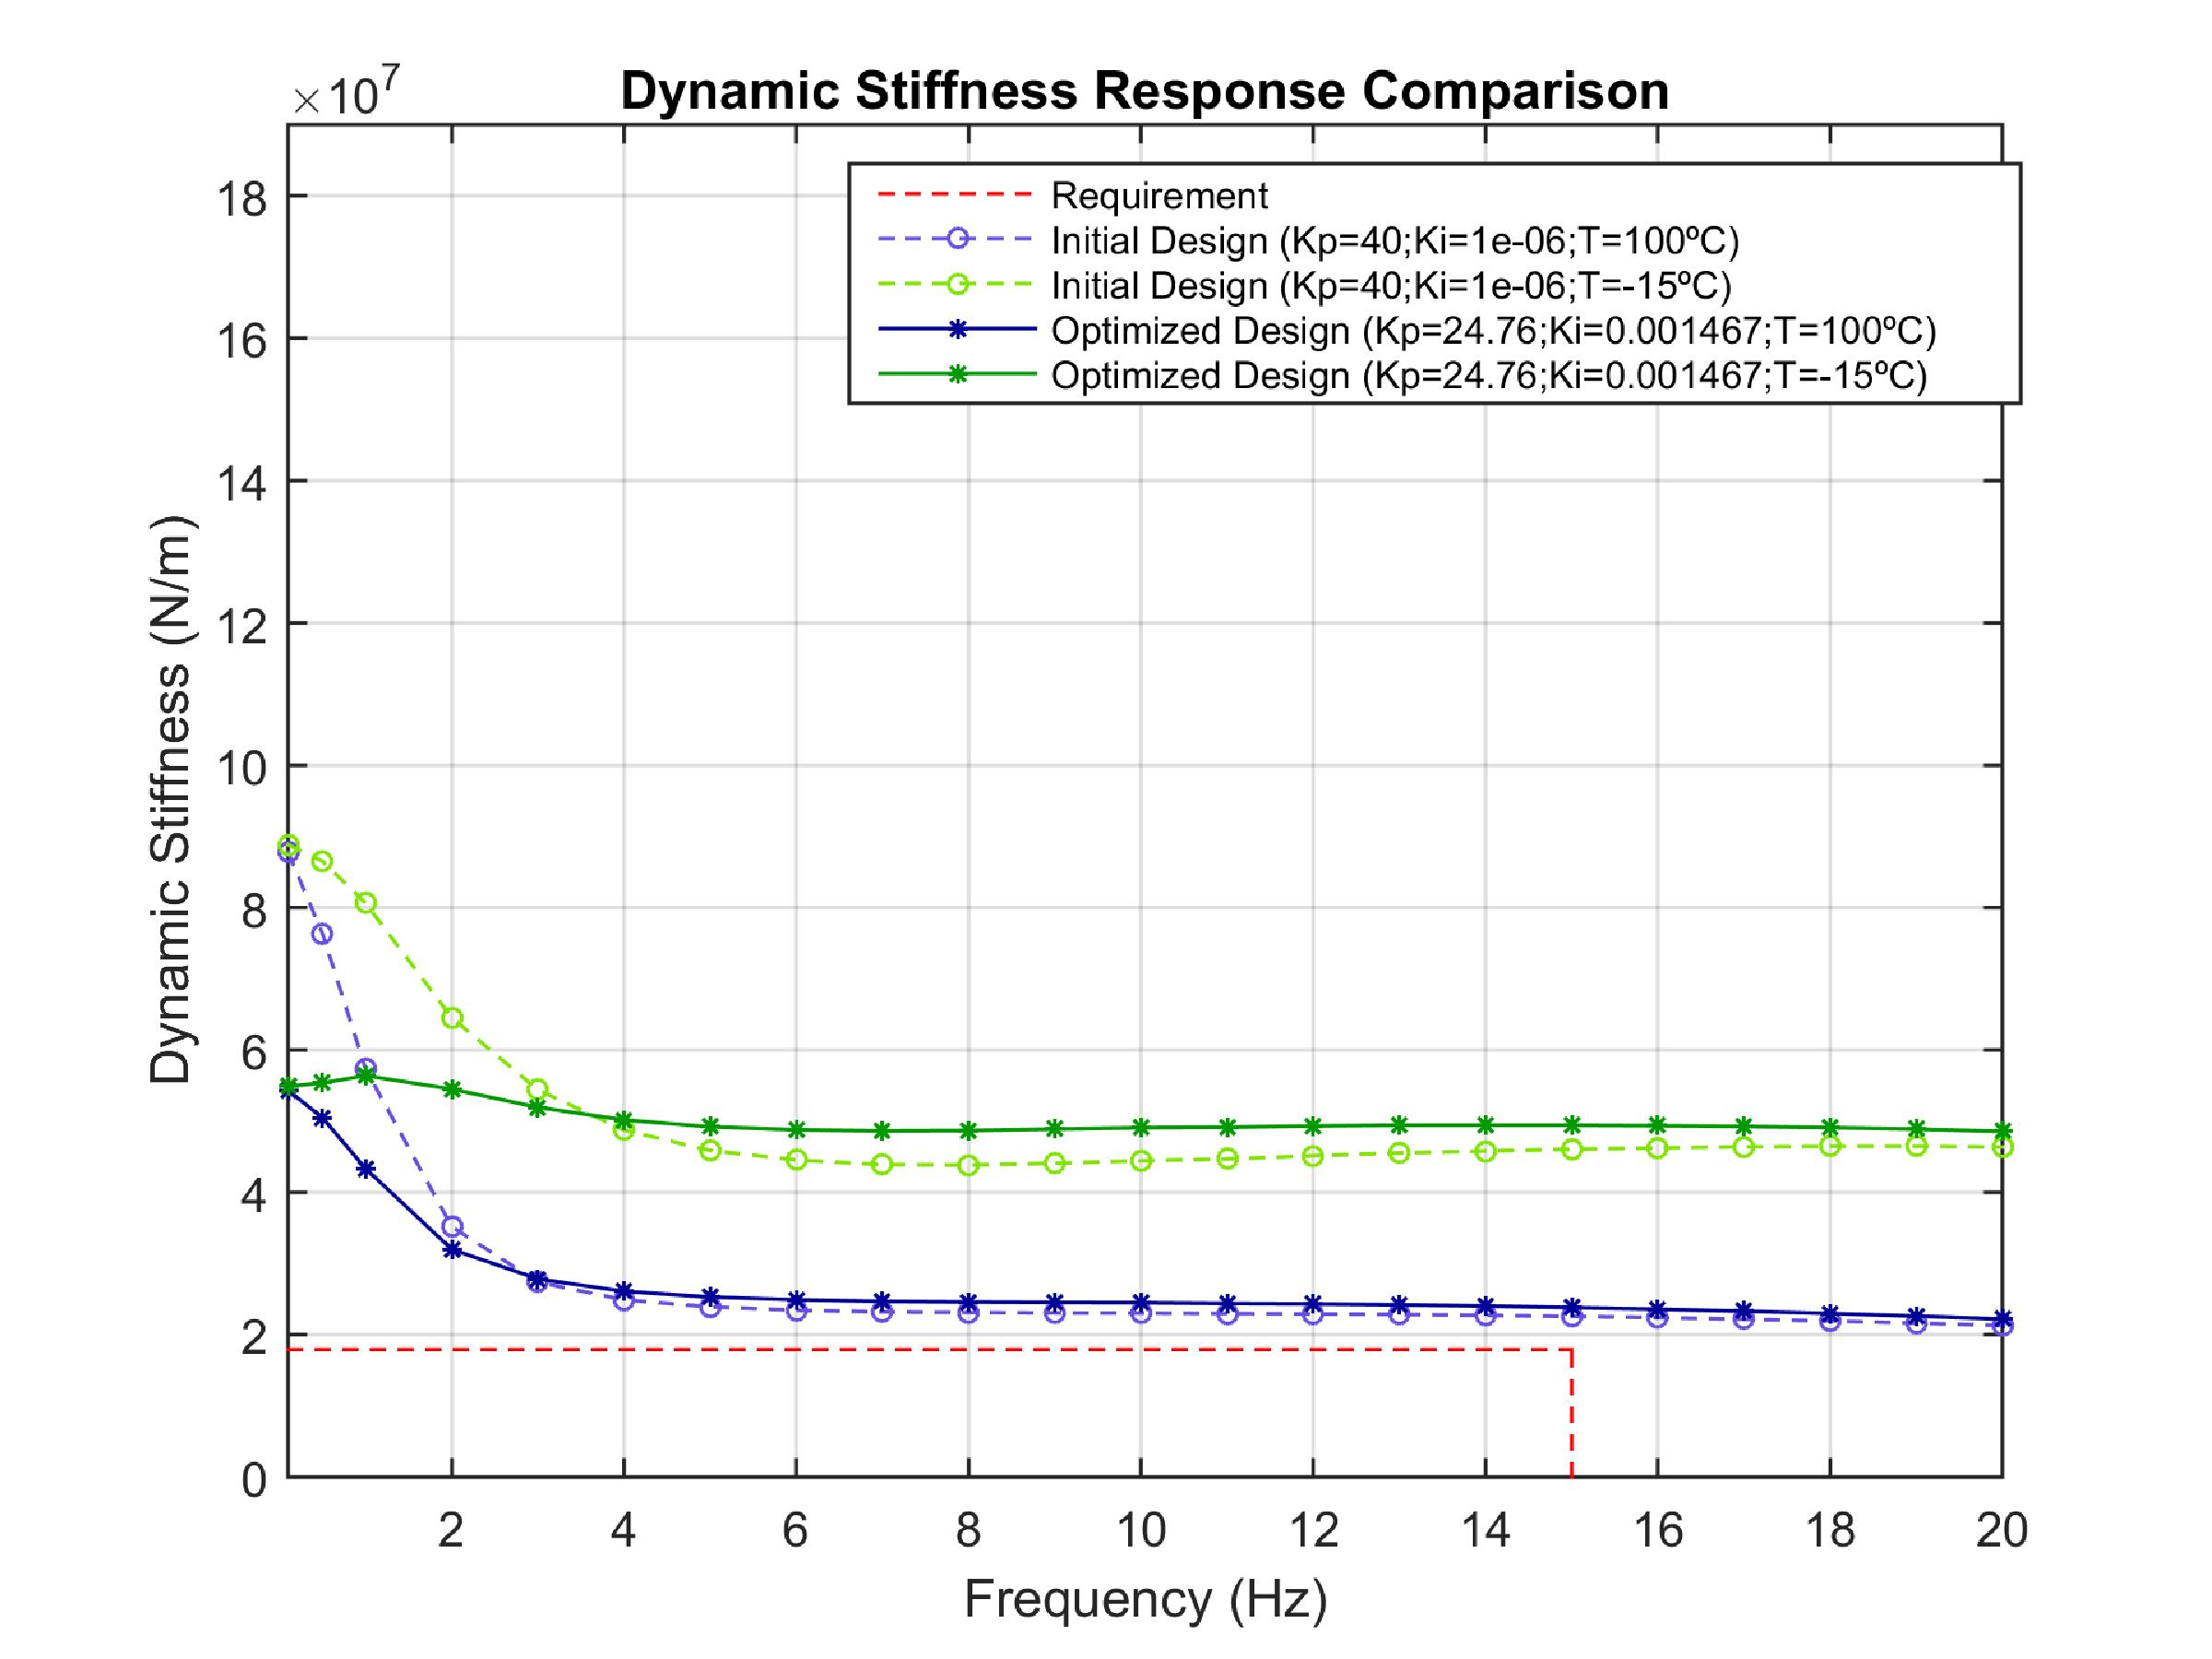
\includegraphics[width=0.9\textwidth]{Figuras/5.OptimizationResults/5-2-2-PI-DynamicStiffnessComparison.jpg}}
	\caption{Dynamic Stiffness Optimization Result for the PI Controller.}
	\label{fig:5_2_2_PI_DynStif}
\end{figure}

Table \ref{table:5_2_2_PI_CostFunctionTable} show the partial values of the cost function for each frequency evaluated by the dynamic stiffness test. As for the P controller, the lower frequencies values are still larger than the higher frequency values.

\begin{table}[H]
	\captionof{table}{PI Controller Final Solution Cost Function for Each Evaluated Frequency}
	\label{table:5_2_2_PI_CostFunctionTable}
	\centering
	\resizebox{14cm}{!} {
		\begin{tabular}{|c|c|c|c|c|c|}
			\hline
			Frequency (Hz) & $J_i$ & Frequency (Hz) & $J_i$ & Frequency (Hz) & $J_i$ \\ \hline
			$0.1$ & $3.64e+07$ & $5$ & $7.39e+06$ & $11$ & $6.48e+06$ \\ \hline
			$0.5$ & $3.25e+07$ & $6$ & $7.01e+06$ & $12$ & $6.42e+06$ \\ \hline
			$1$ & $2.54e+07$ & $7$ & $6.78e+06$ & $13$ & $6.3e+06$ \\ \hline
			$2$ & $1.41e+07$ & $8$ & $6.68e+06$ & $14$ & $6.13e+06$ \\ \hline
			$3$ & $9.93e+06$ & $9$ & $6.63e+06$ & $15$ & $5.91e+06$ \\ \hline
			$4$ & $8.19e+06$ & $10$ & $6.59e+06$ &  &  \\ \hline
	\end{tabular}}
\end{table}

The time response comparison is presented in Figure \ref{fig:5_2_2_PI_TimeResp} and the performance requirements are shown in Table \ref{table:5_2_2_PI_PerfTable}. As observed for proportional controller, the settling time increased by 141ms and the steady state error increased approximately 60\%.

\begin{figure}[H]
	\centering
	\centerline{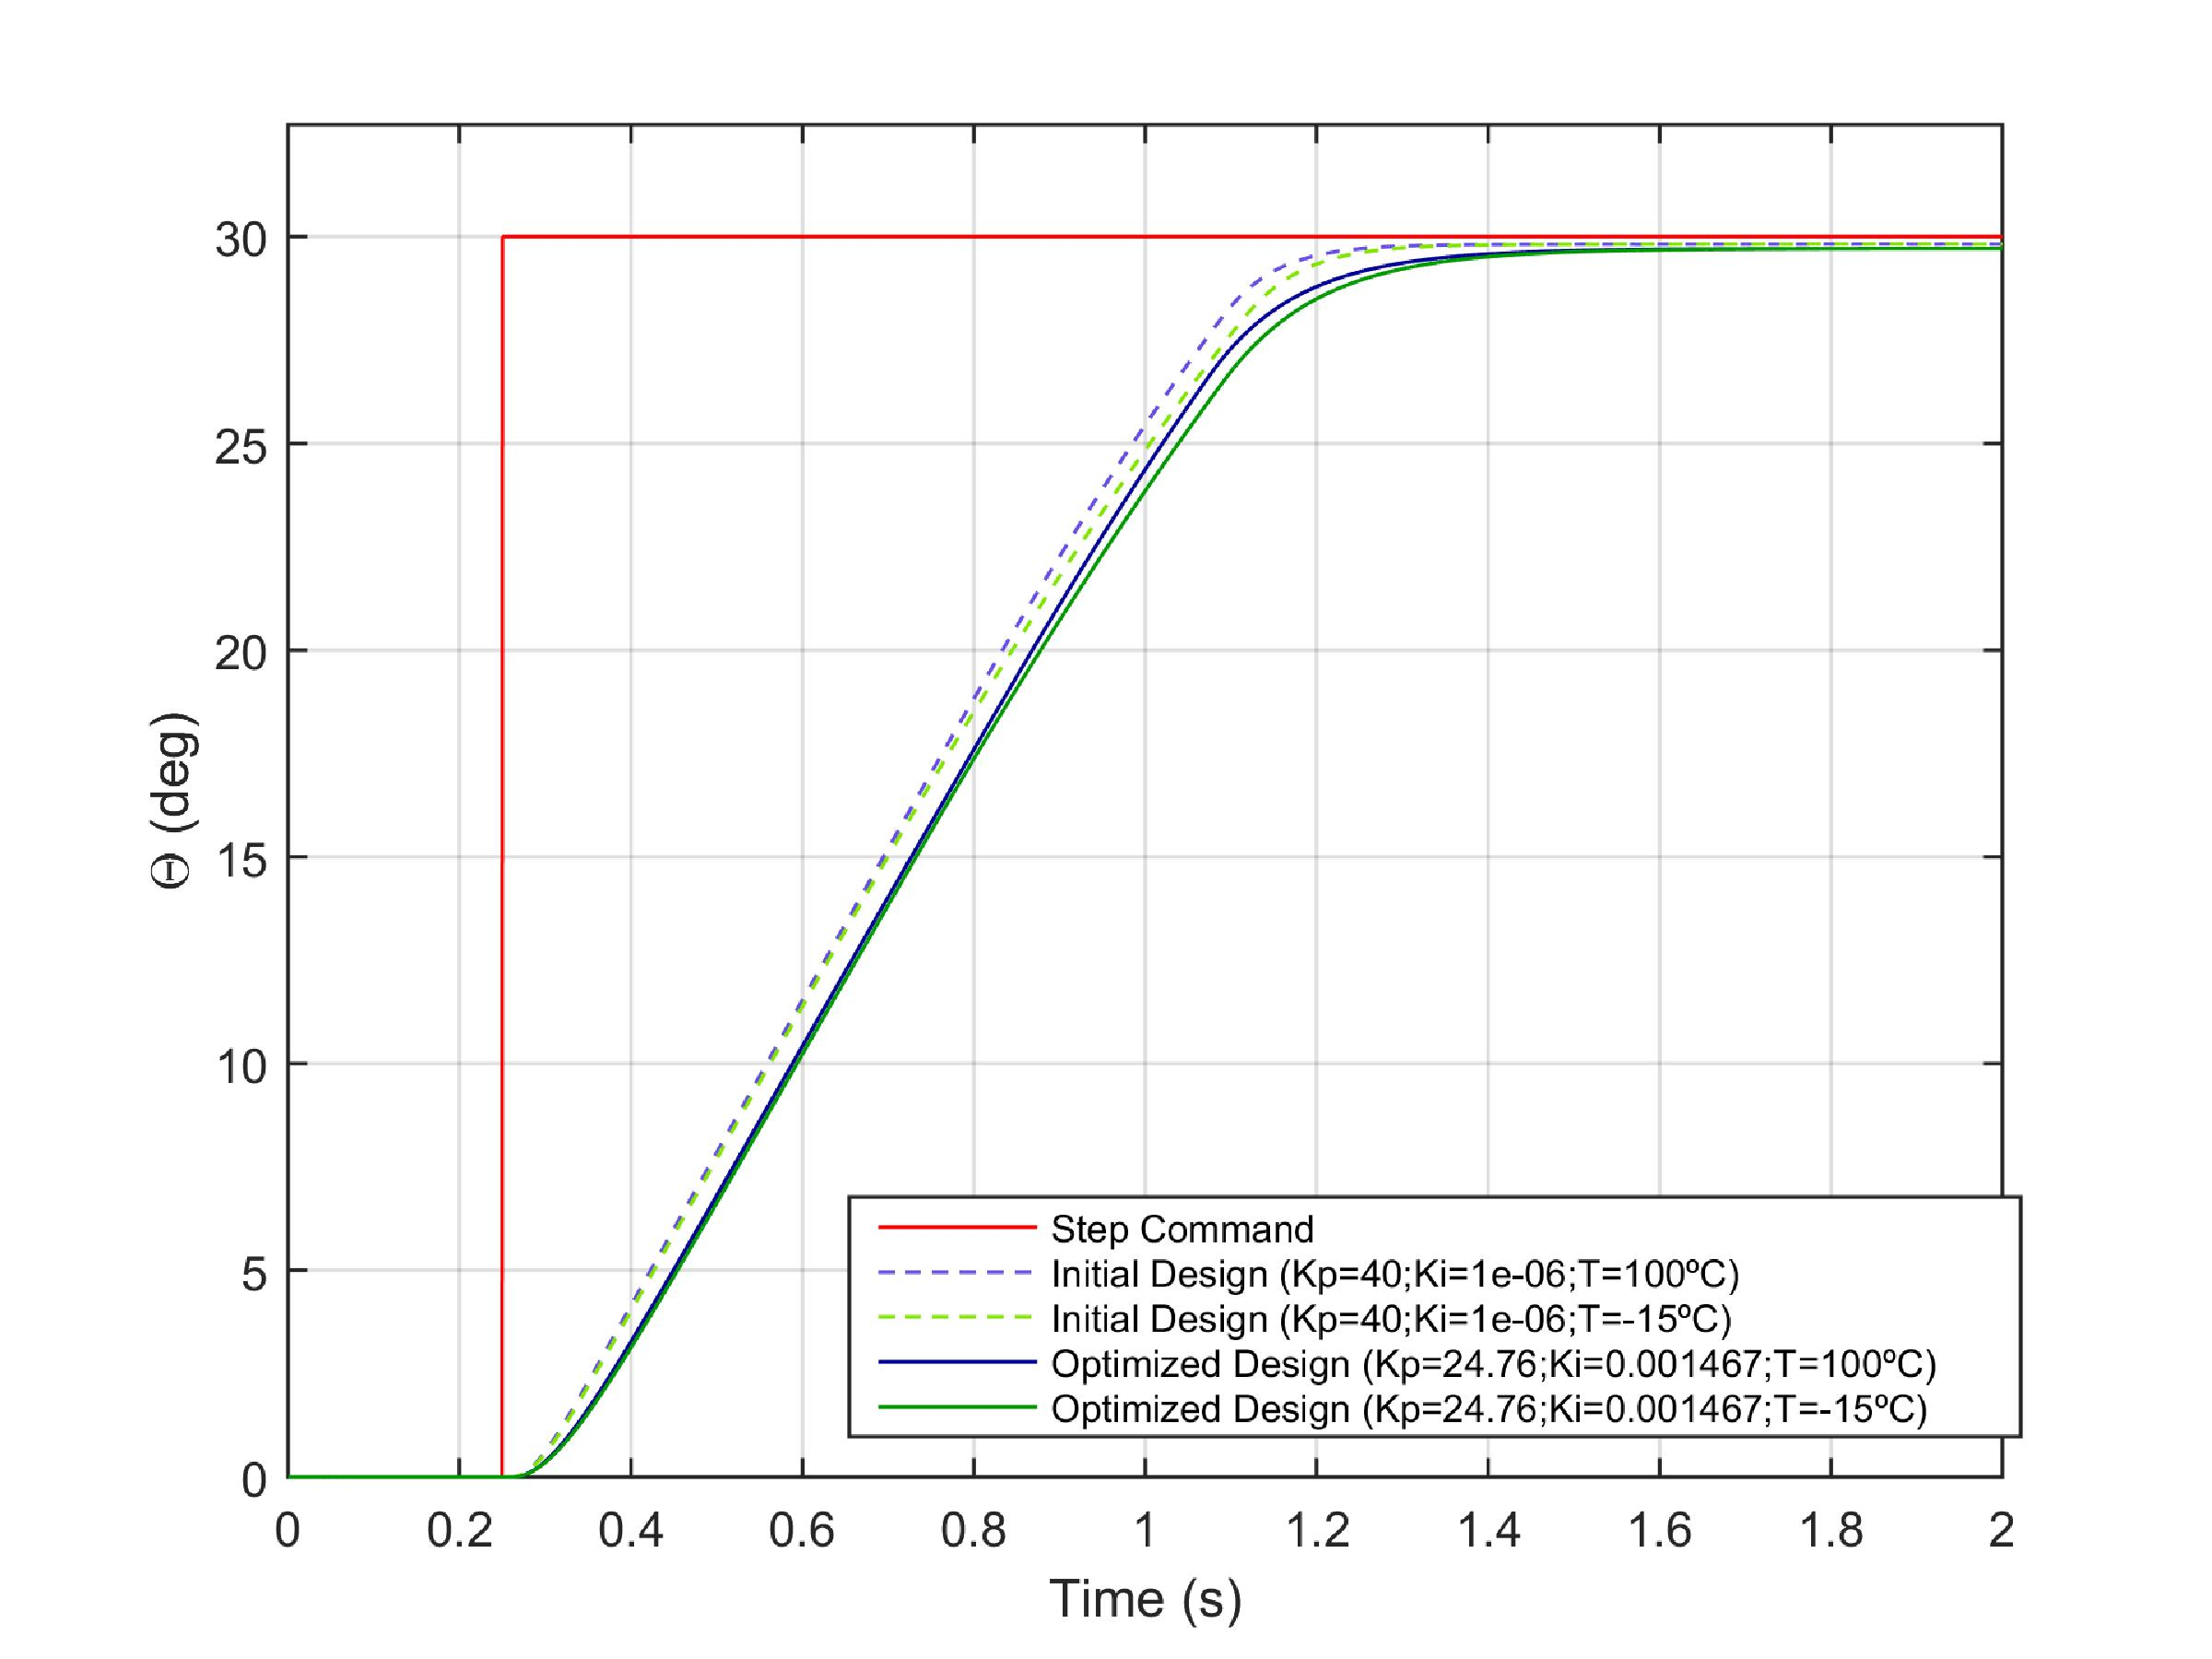
\includegraphics[width=0.9\textwidth]{Figuras/5.OptimizationResults/5-2-2-PI-TimeResponseComparison.jpg}}
	\caption{Time Response Optimization Result for the PI Controller.}
	\label{fig:5_2_2_PI_TimeResp}
\end{figure}

The closed-loop frequency response comparison is presented in Figure \ref{fig:5_2_2_PI_FreqResp} and the performance requirements are also shown in Table \ref{table:5_2_2_PI_PerfTable}. The closed-loop gain allowance increased to 28.19dB  and closed-loop phase allowance remained infinite. Peak magnitude, initial magnitude and bandwidth decreased as expected.

\begin{figure}[H]
	\centering
	\centerline{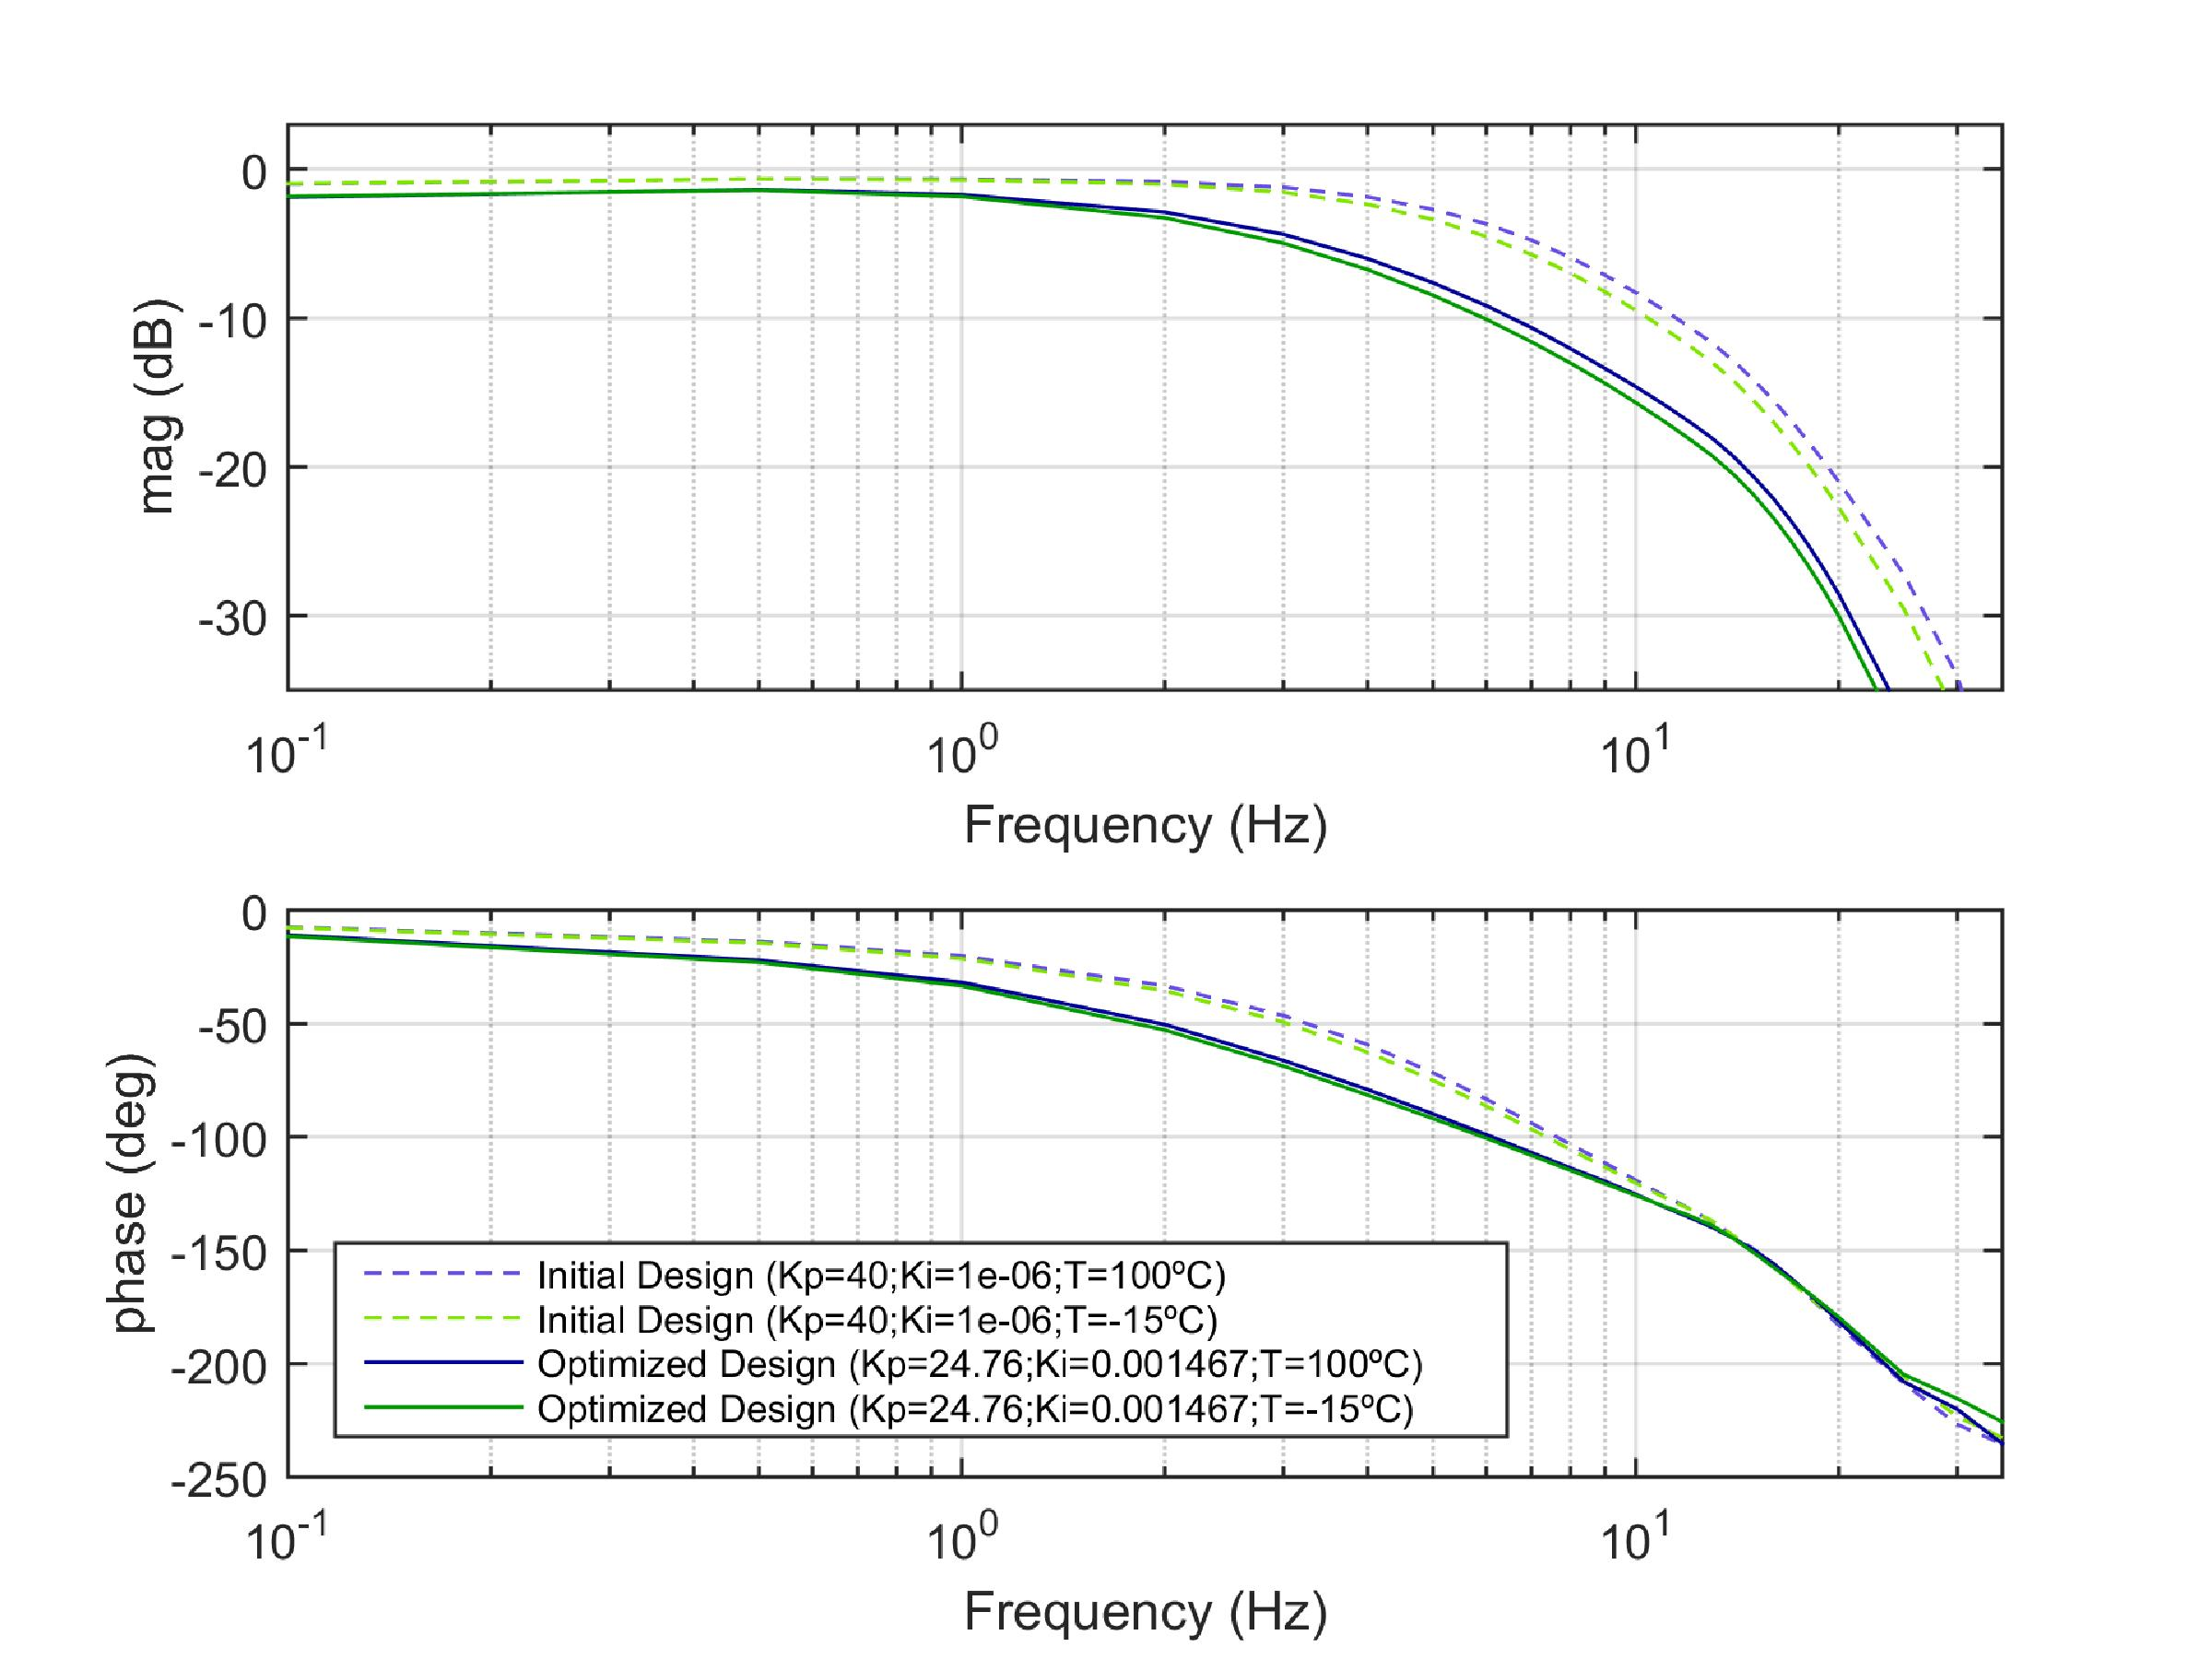
\includegraphics[width=0.9\textwidth]{Figuras/5.OptimizationResults/5-2-2-PI-FrequencyResponseComparison.jpg}}
	\caption{Frequency Response Baseline for the PI Controller.}
	\label{fig:5_2_2_PI_FreqResp}
\end{figure}

\begin{table}[H]
	\captionof{table}{Requirement Compliance for PI Controller}
	\label{table:5_2_2_PI_PerfTable}
	\centering
	\resizebox{14cm}{!} {
		\begin{tabular}{|l|c|c|c|c|}
			\hline
			Design Parameter & Requirement & Baseline & Optimized Controller & Difference (\%) \\ \hline
			Settling Time (ms) & $< 1100$ & $959$ & $1100$ & $14.7$ \\ \hline
			Steady State Error ($\%$) & $< 1$ & $0.27$ & $0.43$ & $59.3$ \\ \hline
			Overshoot ($\%$) & $< 10$ & $0$ & $0$ & $N/A$ \\ \hline
			Minimum Average Rate ($°$/s) & $> 32$ & $34.45$ & $34.09$ & $-1.0$ \\ \hline
			Maximum Average Rate ($°$/s) & $< 36$ & $34.45$ & $34.09$ & $-1.0$ \\ \hline
			Closed-Loop Gain Allowance (dB) & $> 10$ & $20.35$ & $28.19$ & $38.6$ \\ \hline
			Closed-Loop Phase Allowance ($°$) & $> 45$ & $inf$ & $inf$ & $N/A$ \\ \hline
			Closed-Loop Maximum Peak (dB) & $< 0.5$ & $-0.65$ & $-1.38$ & $-112.3$ \\ \hline
			Closed-Loop Initial Magnitude(dB) & $None$ & $-1.0$ & $-1.9$ & $-90.0$ \\ \hline
			Closed-Loop Bandwidth (Hz) & $None$ & $6.3$ & $3.3$ & $-47.6$ \\ \hline
	\end{tabular}}
\end{table}

\subsection{Proportional Derivative Controller (PD)}

The proportional derivative controller optimization execution time was 10.6 hours and required 9 iterations, as per Table \ref{table:5_2_3_PDContExecution}. Also, the optimization yielded a proportional gain of 38.75 and a derivative gain of 0.8134.

\begin{table}[H]
	\captionof{table}{PD Controller Optimization Execution Results}
	\label{table:5_2_3_PDContExecution}
	\centering
	\resizebox{7cm}{!} {
		\begin{tabular}{|l|c|}
			\hline
			Optimized Proportional Gain & 38.75 \\ \hline
			Optimized Derivative Gain & 0.8134 \\ \hline
			Optimization Execution Time (h) & 10.6 \\ \hline
			Number of Iterations & 9 \\ \hline
			Number of Obj. Function Evaluations & 71 \\ \hline			
	\end{tabular}}
\end{table}

The  dynamic stiffness response for each PD design is shown in Figure \ref{fig:5_2_3_PD_DynStif}. Similarly to P and PI controllers, dynamic stiffness increase occurred in frequencies above 1Hz but in this case the gains were smaller, specially at the infinite frequency. 

\begin{figure}[H]
	\centering
	\centerline{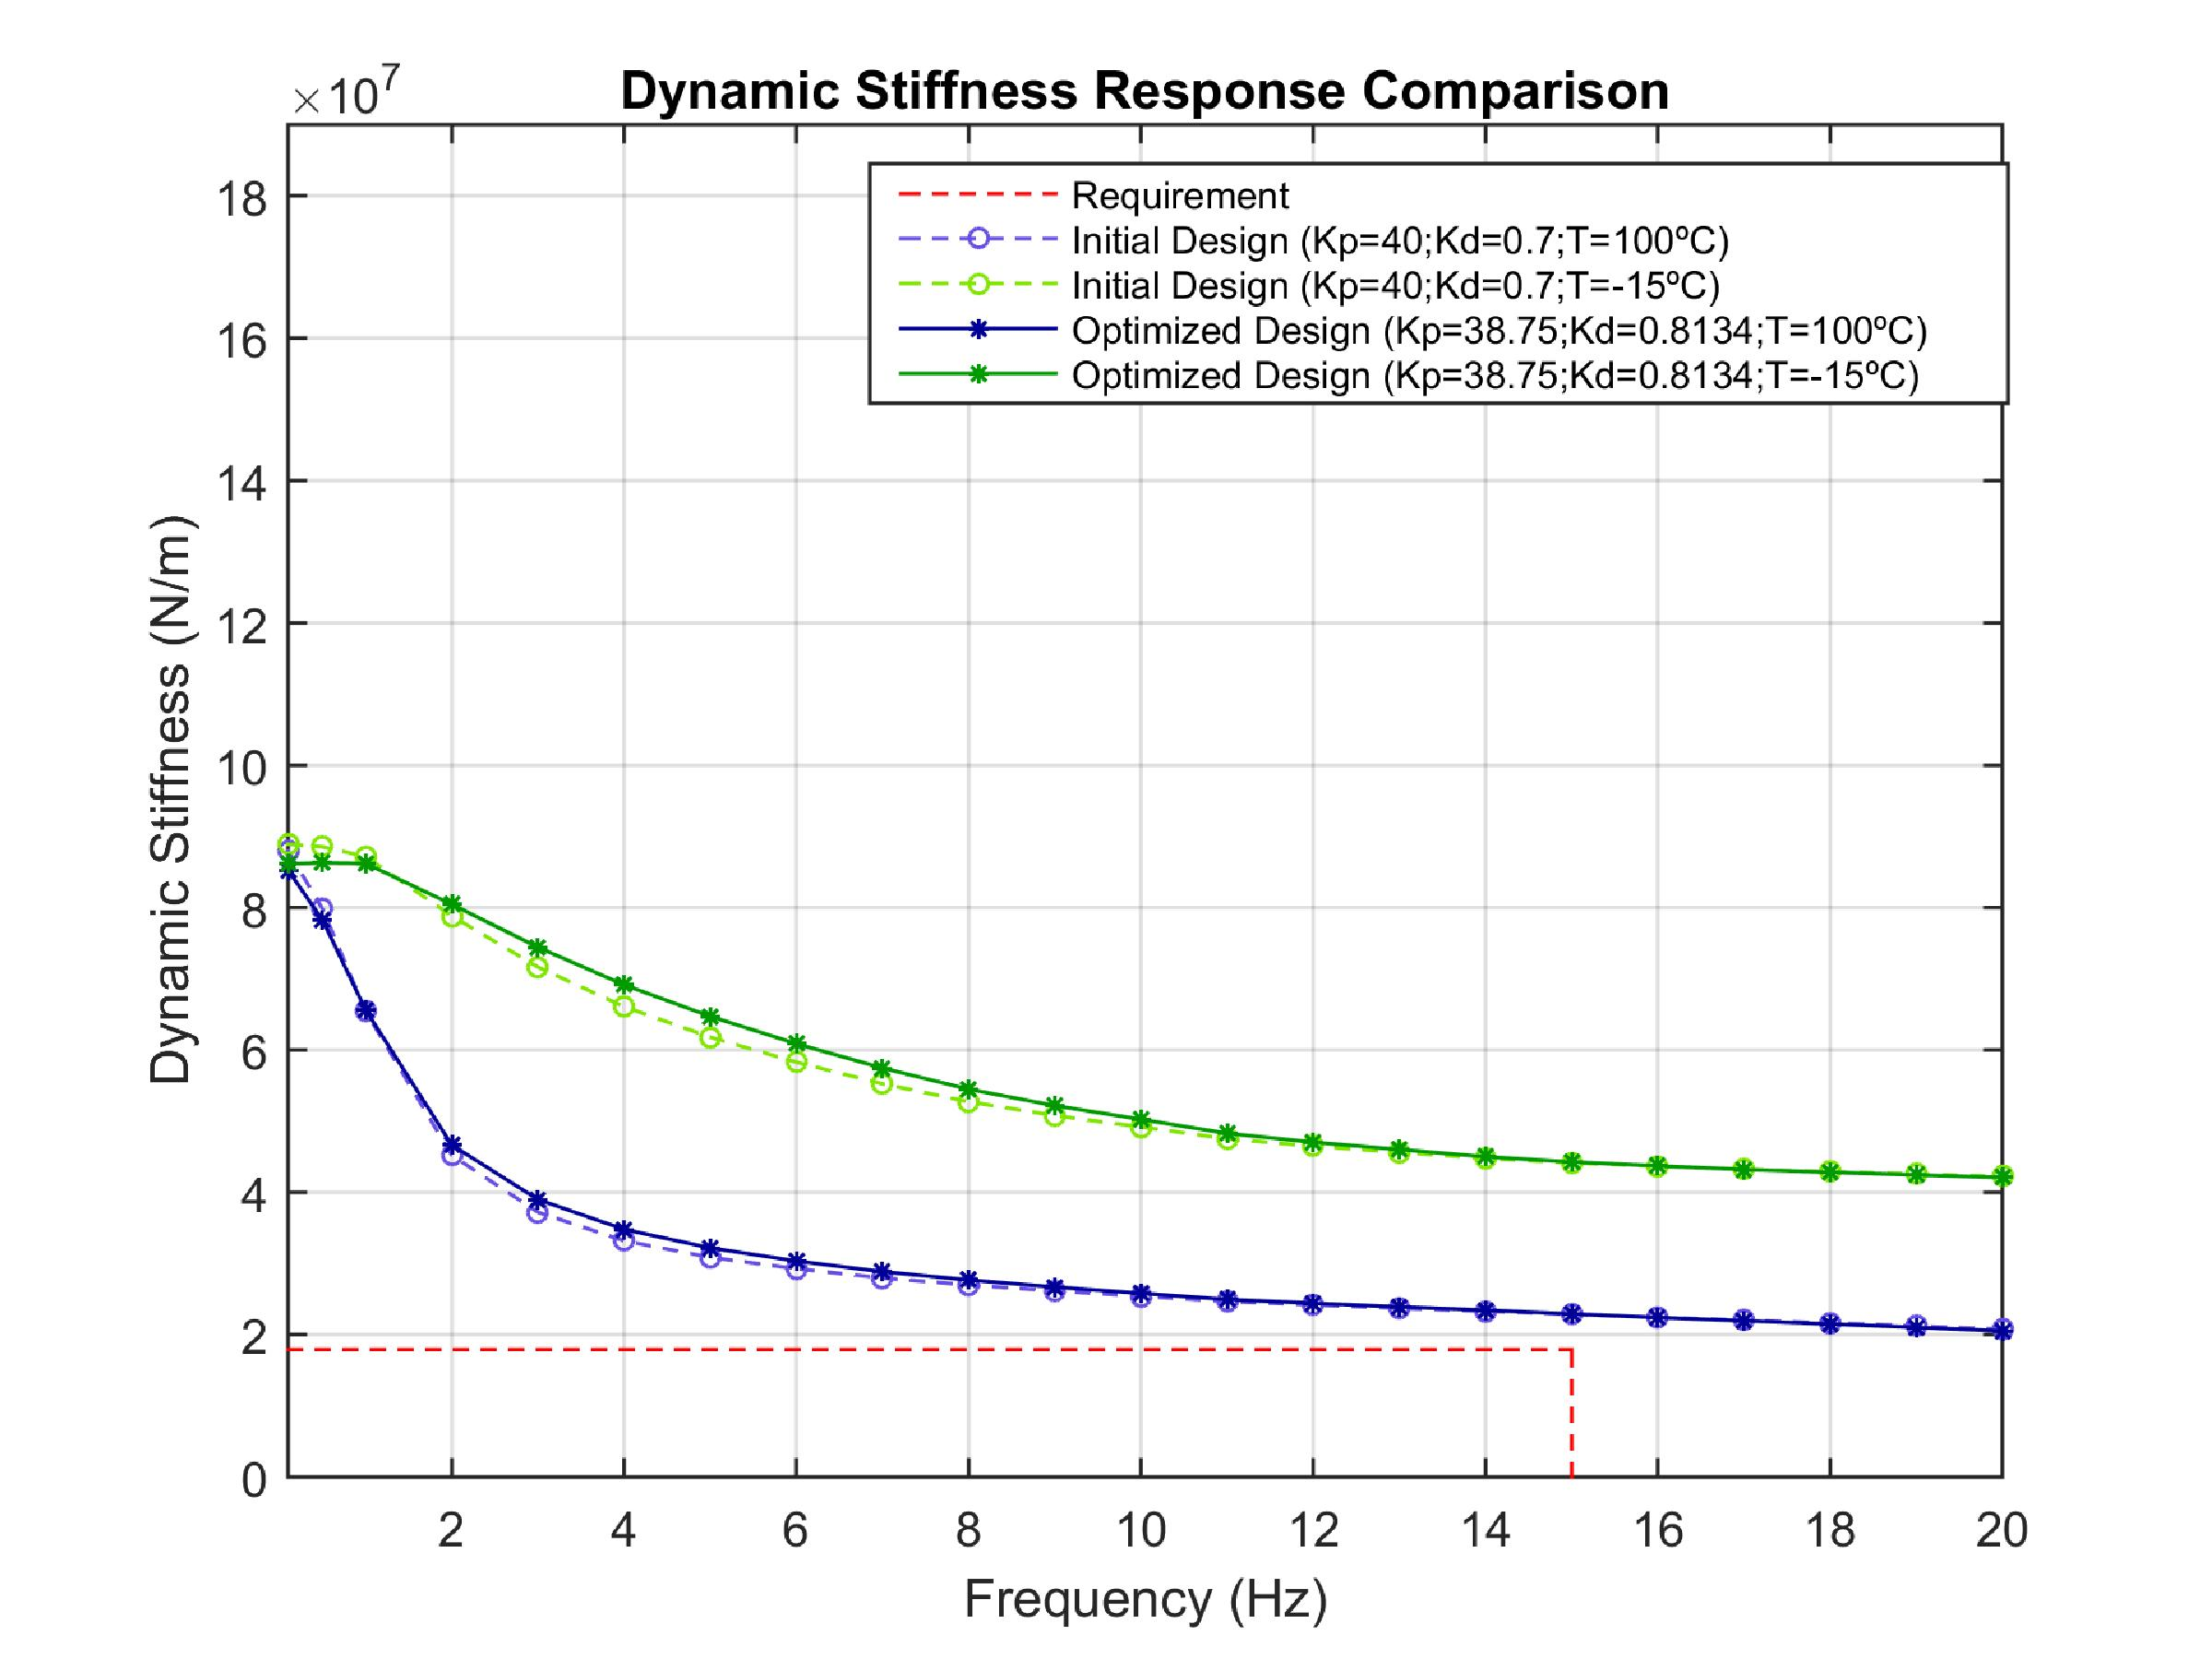
\includegraphics[width=0.9\textwidth]{Figuras/5.OptimizationResults/5-2-3-PD-DynamicStiffnessComparison.jpg}}
	\caption{Dynamic Stiffness Optimization Result for the PD Controller.}
	\label{fig:5_2_3_PD_DynStif}
\end{figure}

Table \ref{table:5_2_3_PD_CostFunctionTable} show the partial values of the cost function for each frequency evaluated by the dynamic stiffness test. The lower frequencies values are larger since the dynamic stiffness is still greater in this range. 

\begin{table}[H]
	\captionof{table}{PD Controller Final Solution Cost Function for Each Evaluated Frequency}
	\label{table:5_2_3_PD_CostFunctionTable}
	\centering
	\resizebox{14cm}{!} {
		\begin{tabular}{|c|c|c|c|c|c|}
			\hline
			Frequency (Hz) & $J_i$ & Frequency (Hz) & $J_i$ & Frequency (Hz) & $J_i$ \\ \hline
			$0.1$ & $6.73e+07$ & $5$ & $1.43e+07$ & $11$ & $7.05e+06$ \\ \hline
			$0.5$ & $6.03e+07$ & $6$ & $1.24e+07$ & $12$ & $6.52e+06$ \\ \hline
			$1$ & $4.77e+07$ & $7$ & $1.09e+07$ & $13$ & $6.01e+06$ \\ \hline
			$2$ & $2.87e+07$ & $8$ & $9.79e+06$ & $14$ & $5.55e+06$ \\ \hline
			$3$ & $2.11e+07$ & $9$ & $8.79e+06$ & $15$ & $5.02e+06$ \\ \hline
			$4$ & $1.69e+07$ & $10$ & $7.92e+06$ &  &  \\ \hline
	\end{tabular}}
\end{table}

The time response comparison is presented in Figure \ref{fig:5_2_3_PD_TimeResp} and the performance requirements are shown in Table \ref{table:5_2_3_PD_PerfTable}. The settling time increased by 14ms and the steady state error did not change.

\begin{figure}[H]
	\centering
	\centerline{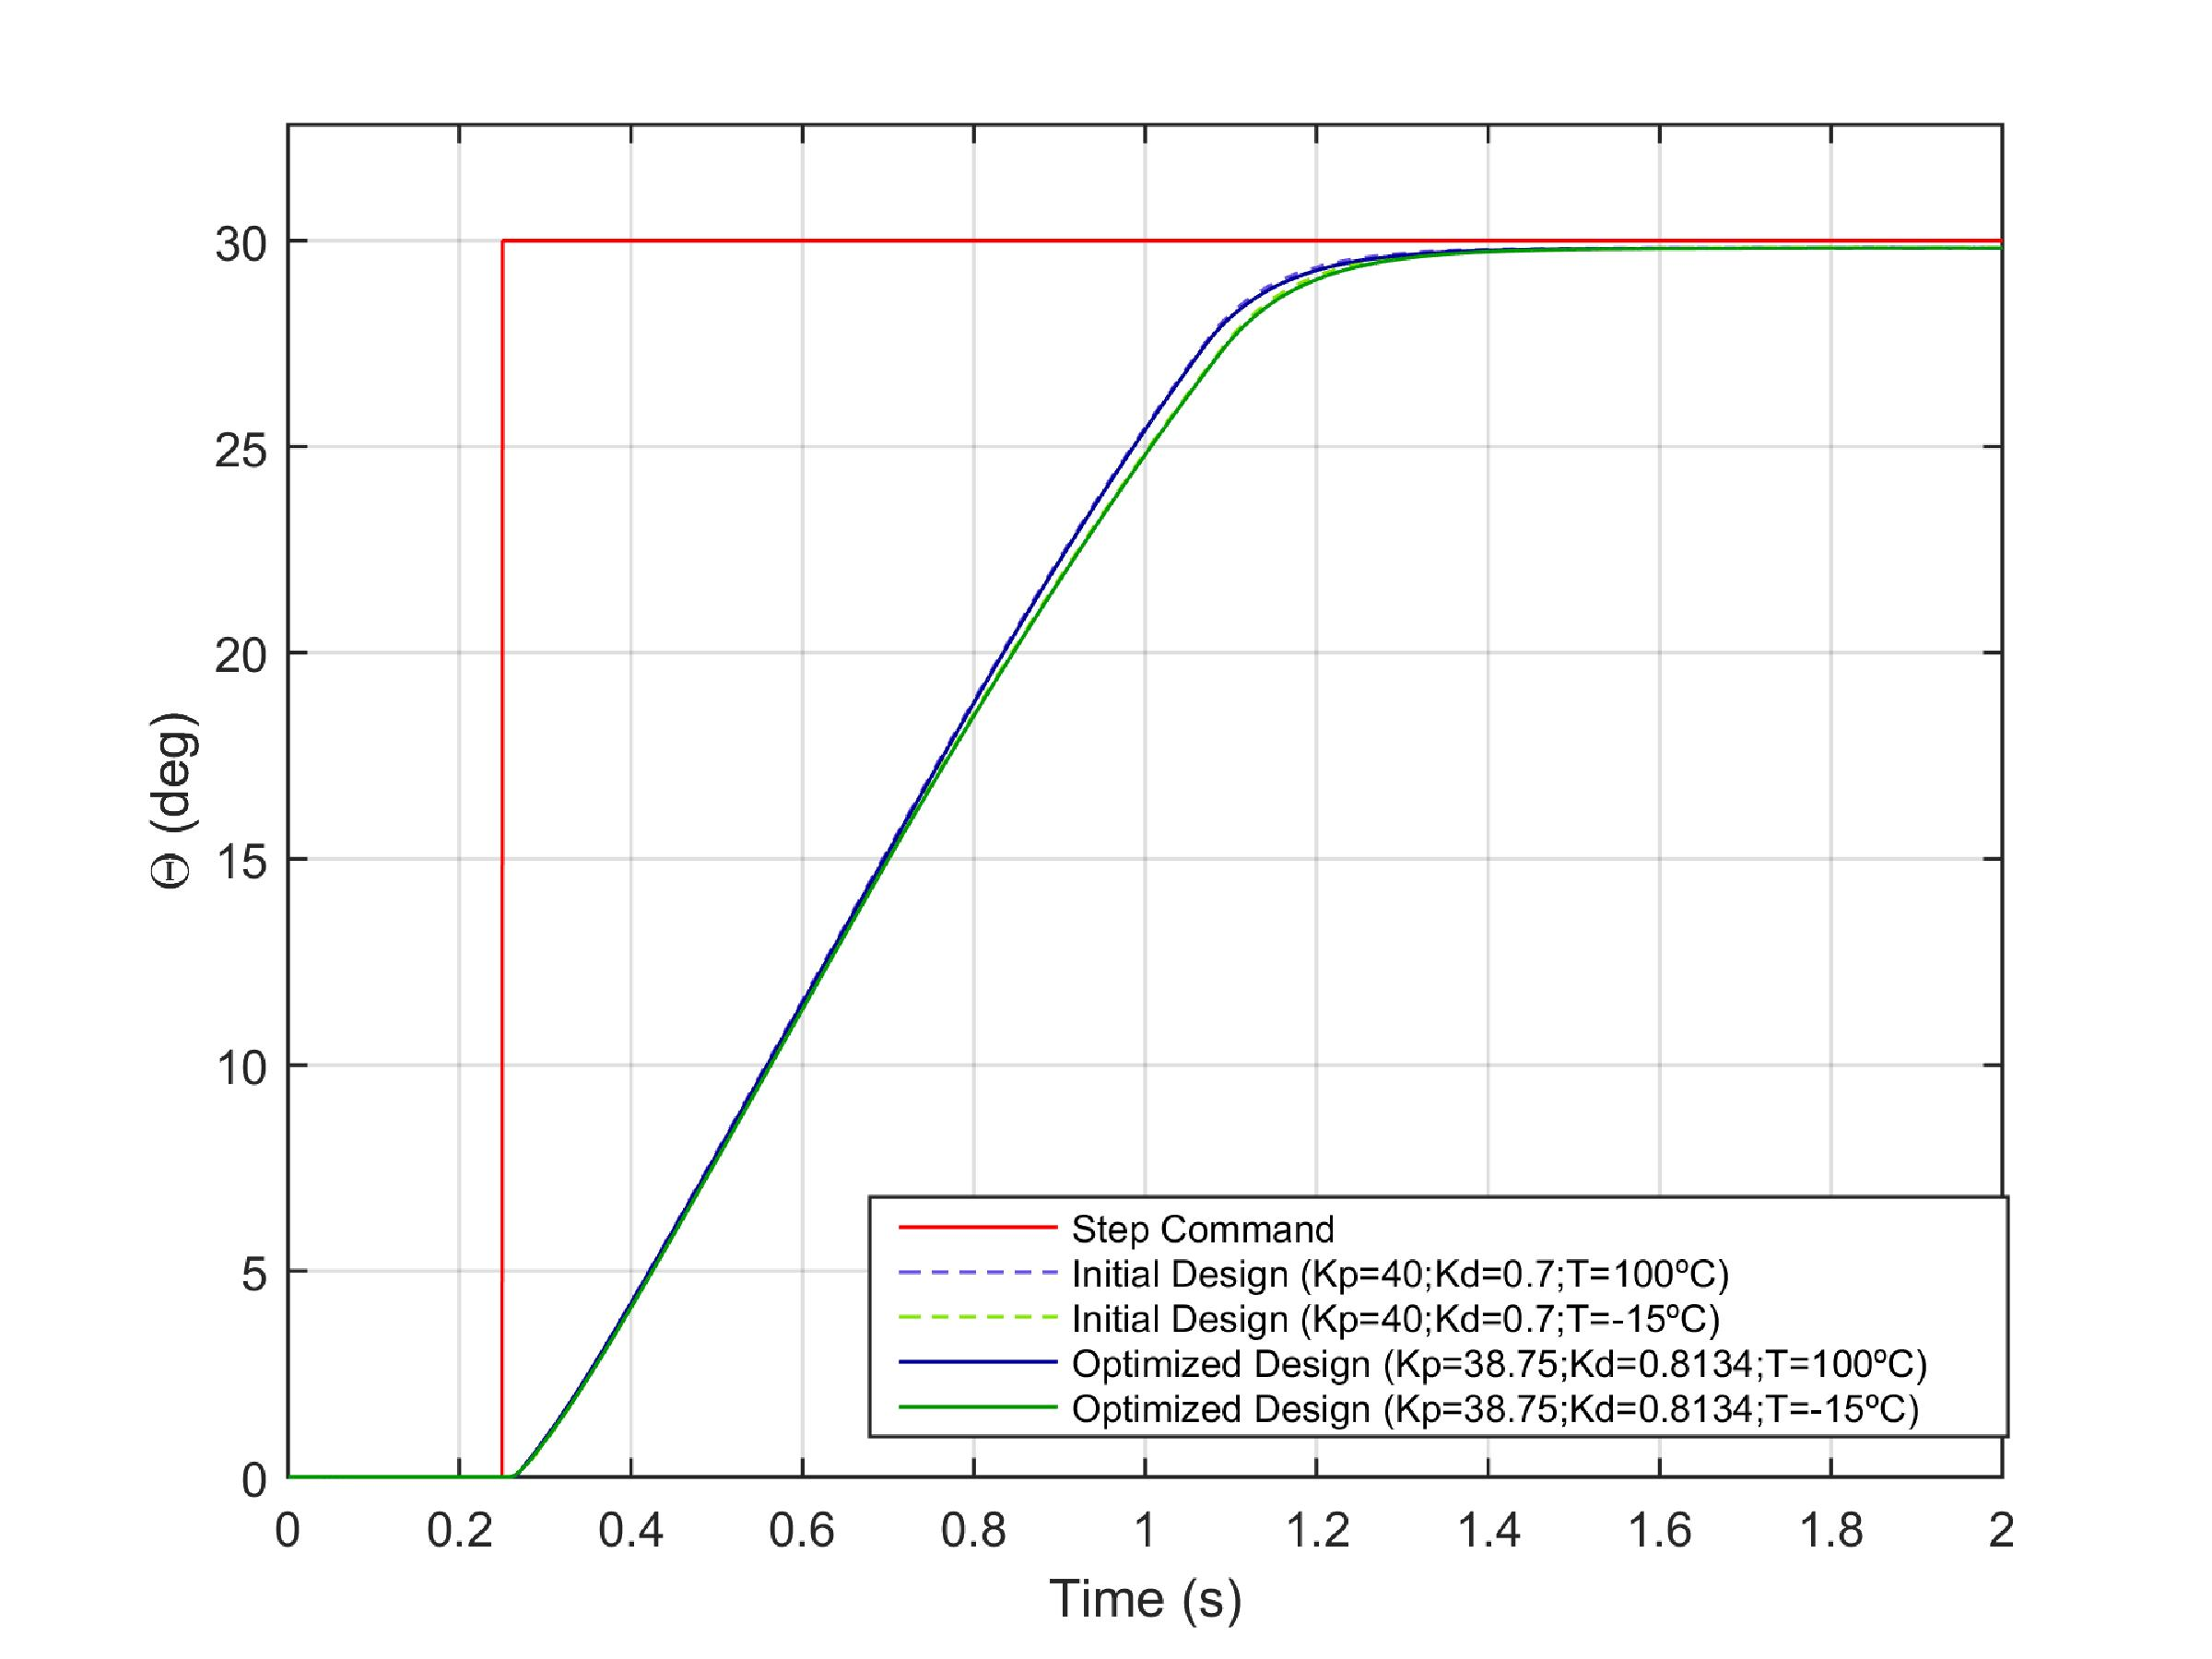
\includegraphics[width=0.9\textwidth]{Figuras/5.OptimizationResults/5-2-3-PD-TimeResponseComparison.jpg}}
	\caption{Time Response Optimization Result for the PD Controller.}
	\label{fig:5_2_3_PD_TimeResp}
\end{figure}

\begin{figure}[H]
	\centering
	\centerline{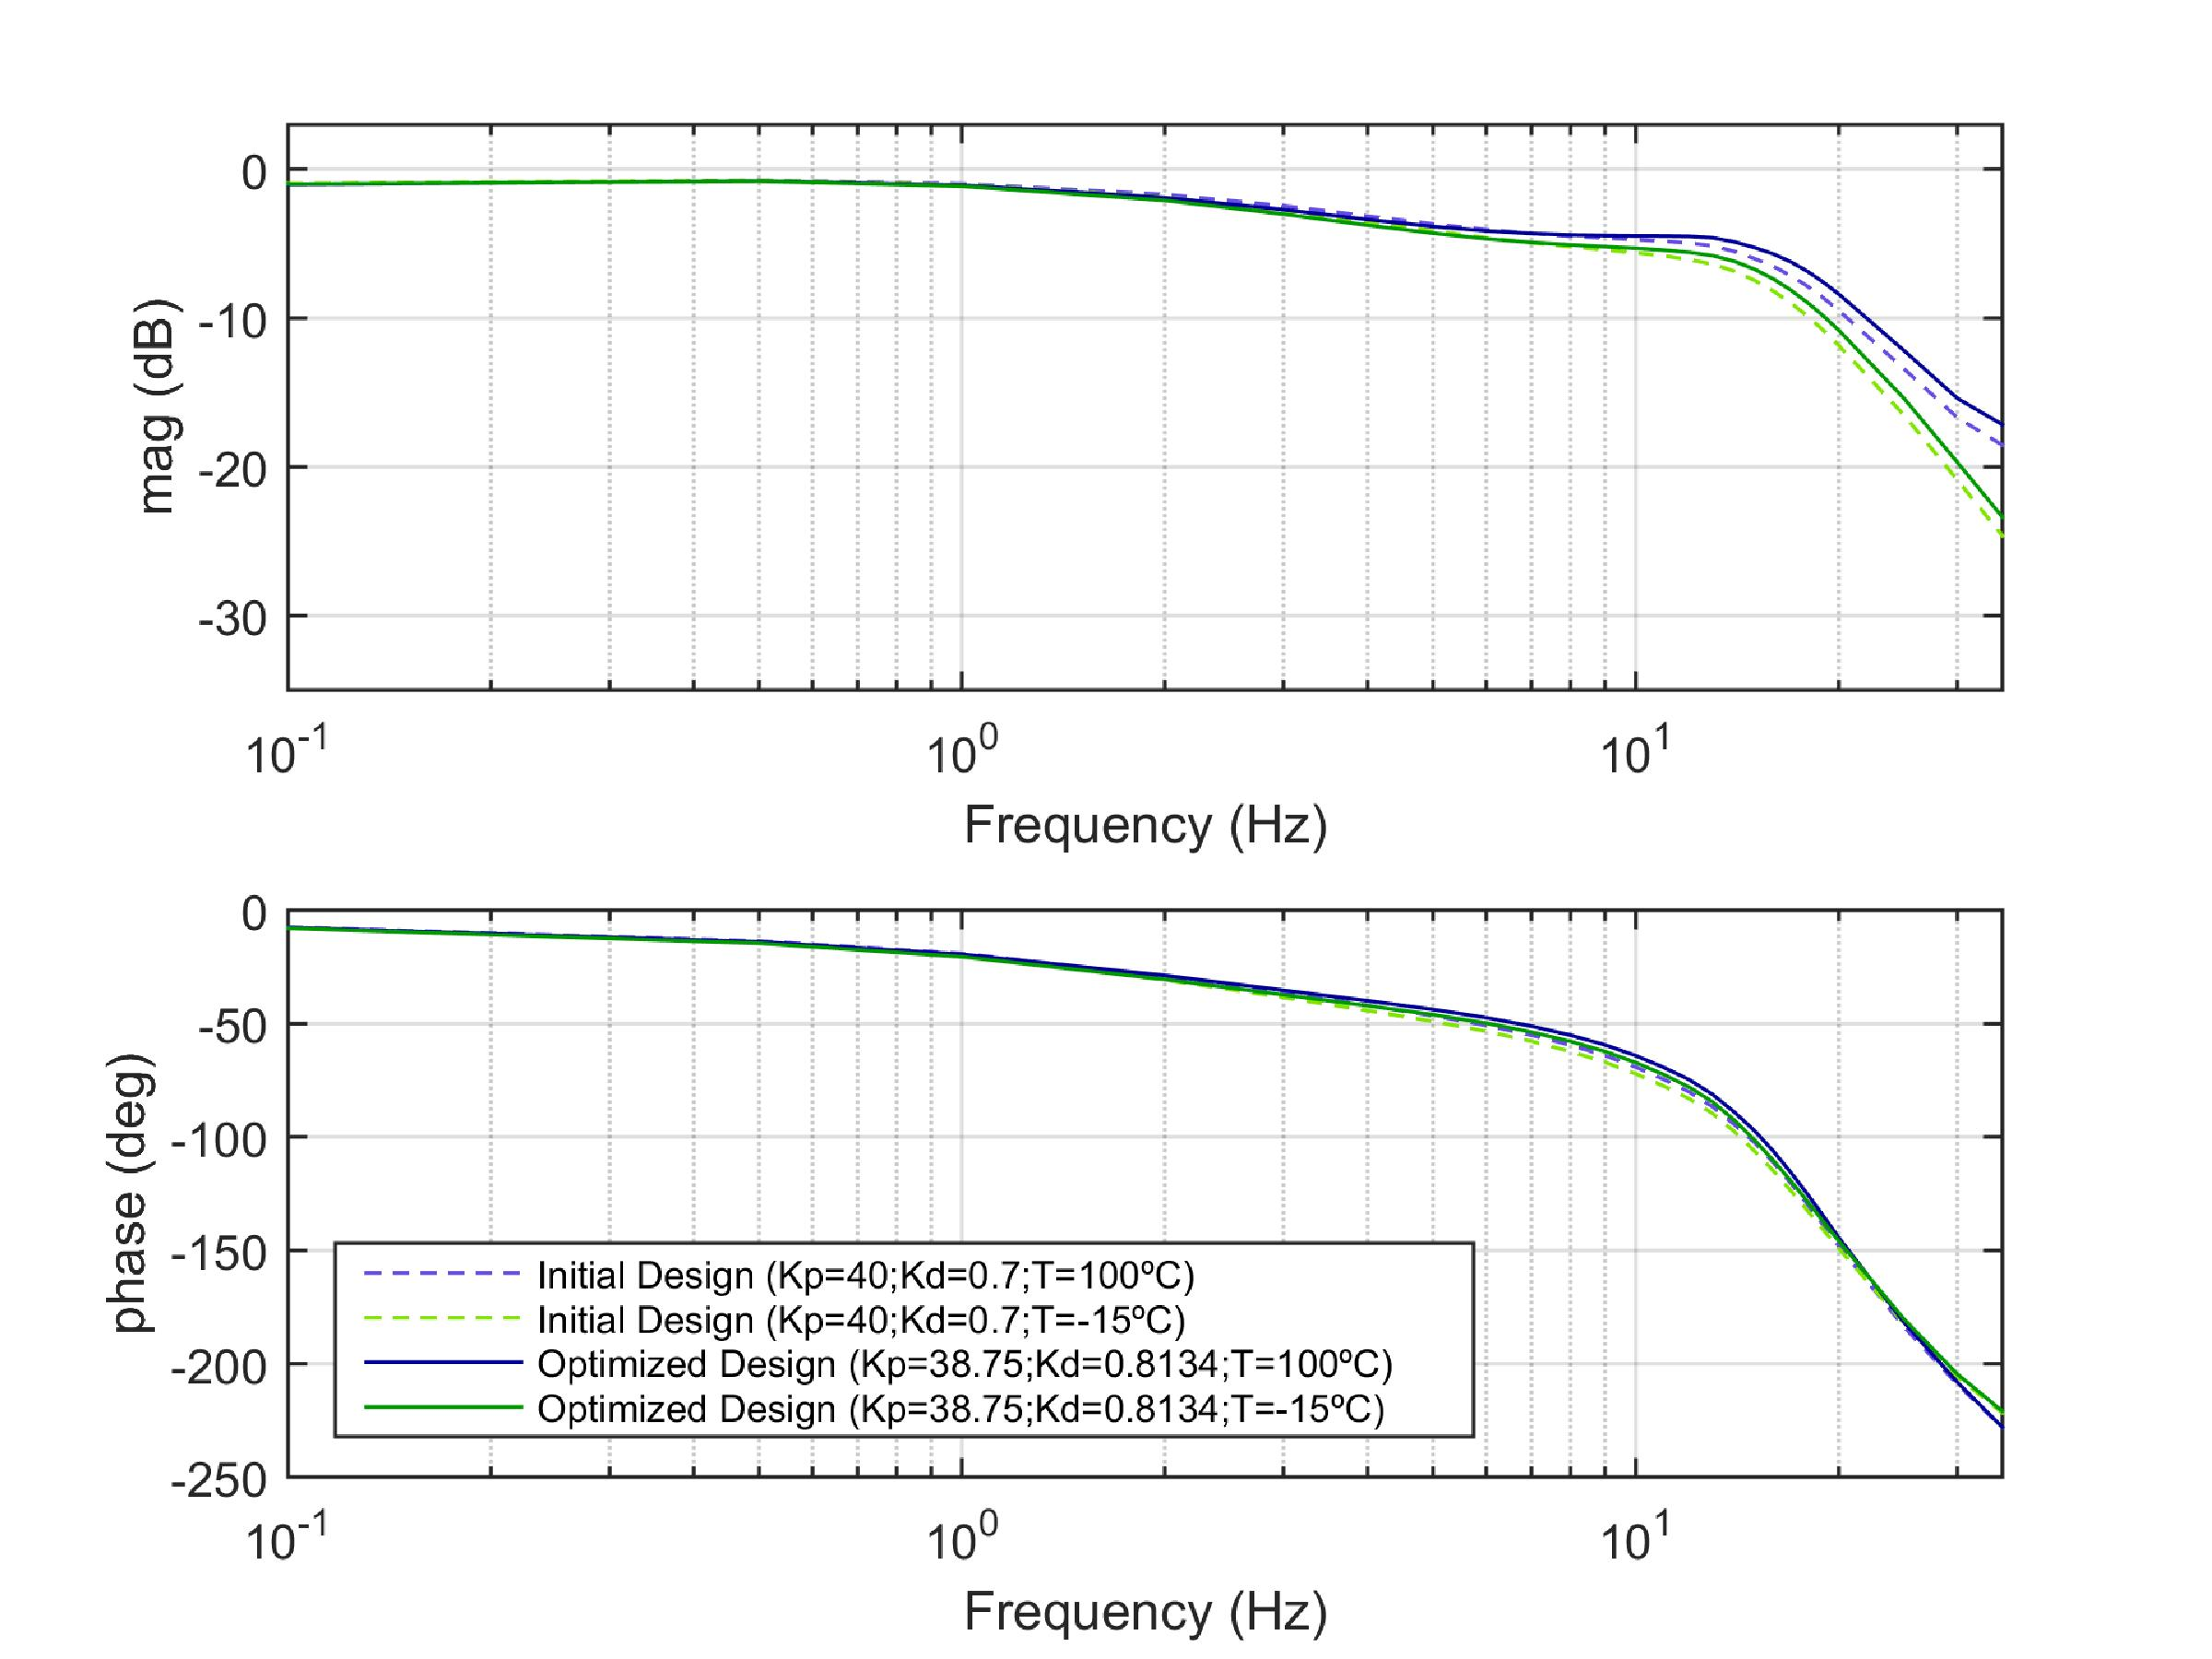
\includegraphics[width=0.9\textwidth]{Figuras/5.OptimizationResults/5-2-3-PD-FrequencyResponseComparison.jpg}}
	\caption{Frequency Response Baseline for the PD Controller.}
	\label{fig:5_2_3_PD_FreqResp}
\end{figure}

The closed-loop frequency response comparison is presented in Figure \ref{fig:5_2_3_PD_FreqResp} and the performance requirements are also shown in Table \ref{table:5_2_3_PD_PerfTable}. The closed-loop gain allowance was slightly reduced but the closed-loop phase allowance remained infinite. Other performance parameters did not change significantly.

The optimization result in this case is different from all previously obtained. None of the parameters in Table \ref{table:5_2_3_PD_PerfTable} were close to the requirement, unlike the previous results in which at least one parameter either violated or was equal to the requirement. This suggests that in this case the optimization algorithm found a local minimum, a solution in which all of its neighbors have a greater objective function than itself.

\begin{table}[H]
	\captionof{table}{Requirement Compliance for PD Controller}
	\label{table:5_2_3_PD_PerfTable}
	\centering
	\resizebox{14cm}{!} {
		\begin{tabular}{|l|c|c|c|c|}
			\hline
			Design Parameter & Requirement & Baseline & Optimized Controller & Difference (\%) \\ \hline
			Settling Time (ms) & $< 1100$ & $992$ & $1006$ & $1.4$ \\ \hline
			Steady State Error ($\%$) & $< 1$ & $0.27$ & $0.28$ & $3.7$ \\ \hline
			Overshoot ($\%$) & $< 10$ & $0$ & $0$ & $N/A$ \\ \hline
			Minimum Average Rate ($°$/s) & $> 32$ & $34.32$ & $34.27$ & $-0.1$ \\ \hline
			Maximum Average Rate ($°$/s) & $< 36$ & $34.32$ & $34.27$ & $-0.1$ \\ \hline
			Closed-Loop Gain Allowance (dB) & $> 10$ & $13$ & $12$ & $-7.7$ \\ \hline
			Closed-Loop Phase Allowance ($°$) & $> 45$ & $inf$ & $inf$ & $N/A$ \\ \hline
			Closed-Loop Maximum Peak (dB) & $< 0.5$ & $-0.74$ & $-0.79$ & $-6.8$ \\ \hline
			Closed-Loop Initial Magnitude(dB) & $None$ & $-0.99$ & $-1.03$ & $-4.0$ \\ \hline
			Closed-Loop Bandwidth (Hz) & $None$ & $5.8$ & $5.6$ & $-3.9$ \\ \hline
	\end{tabular}}
\end{table}

\subsection{Proportional Integral Derivative Controller (PID)}

The proportional integral derivative controller optimization execution time was 9.9 hours and required 9 iterations, as per Table \ref{table:5_2_4_PIDContExecution}. Also, the optimization yielded a proportional gain of 39.21, integral gain of 7.005e-4 and a derivative gain of 0.8067. These values were evaluated separately by \citeonline{Ballesteros} but were not considered together as a PID design.

\begin{table}[H]
	\captionof{table}{PID Controller Optimization Execution Results}
	\label{table:5_2_4_PIDContExecution}
	\centering
	\resizebox{7cm}{!} {
		\begin{tabular}{|l|c|}
			\hline
			Optimized Proportional Gain & 39.21 \\ \hline
			Optimized Integral Gain & 7.005e-4 \\ \hline
			Optimized Derivative Gain & 0.8067 \\ \hline
			Optimization Execution Time (h) & 9.9 \\ \hline
			Number of Iterations & 9 \\ \hline	
			Number of Obj. Function Evaluations & 64 \\ \hline	
	\end{tabular}}
\end{table}

The  dynamic stiffness response for each PID design is shown in Figure \ref{fig:5_2_4_PID_DynStif}. Similarly to the PD controller, increase in dynamic stiffness was observed in frequencies above 1Hz.

\begin{figure}[H]
	\centering
	\centerline{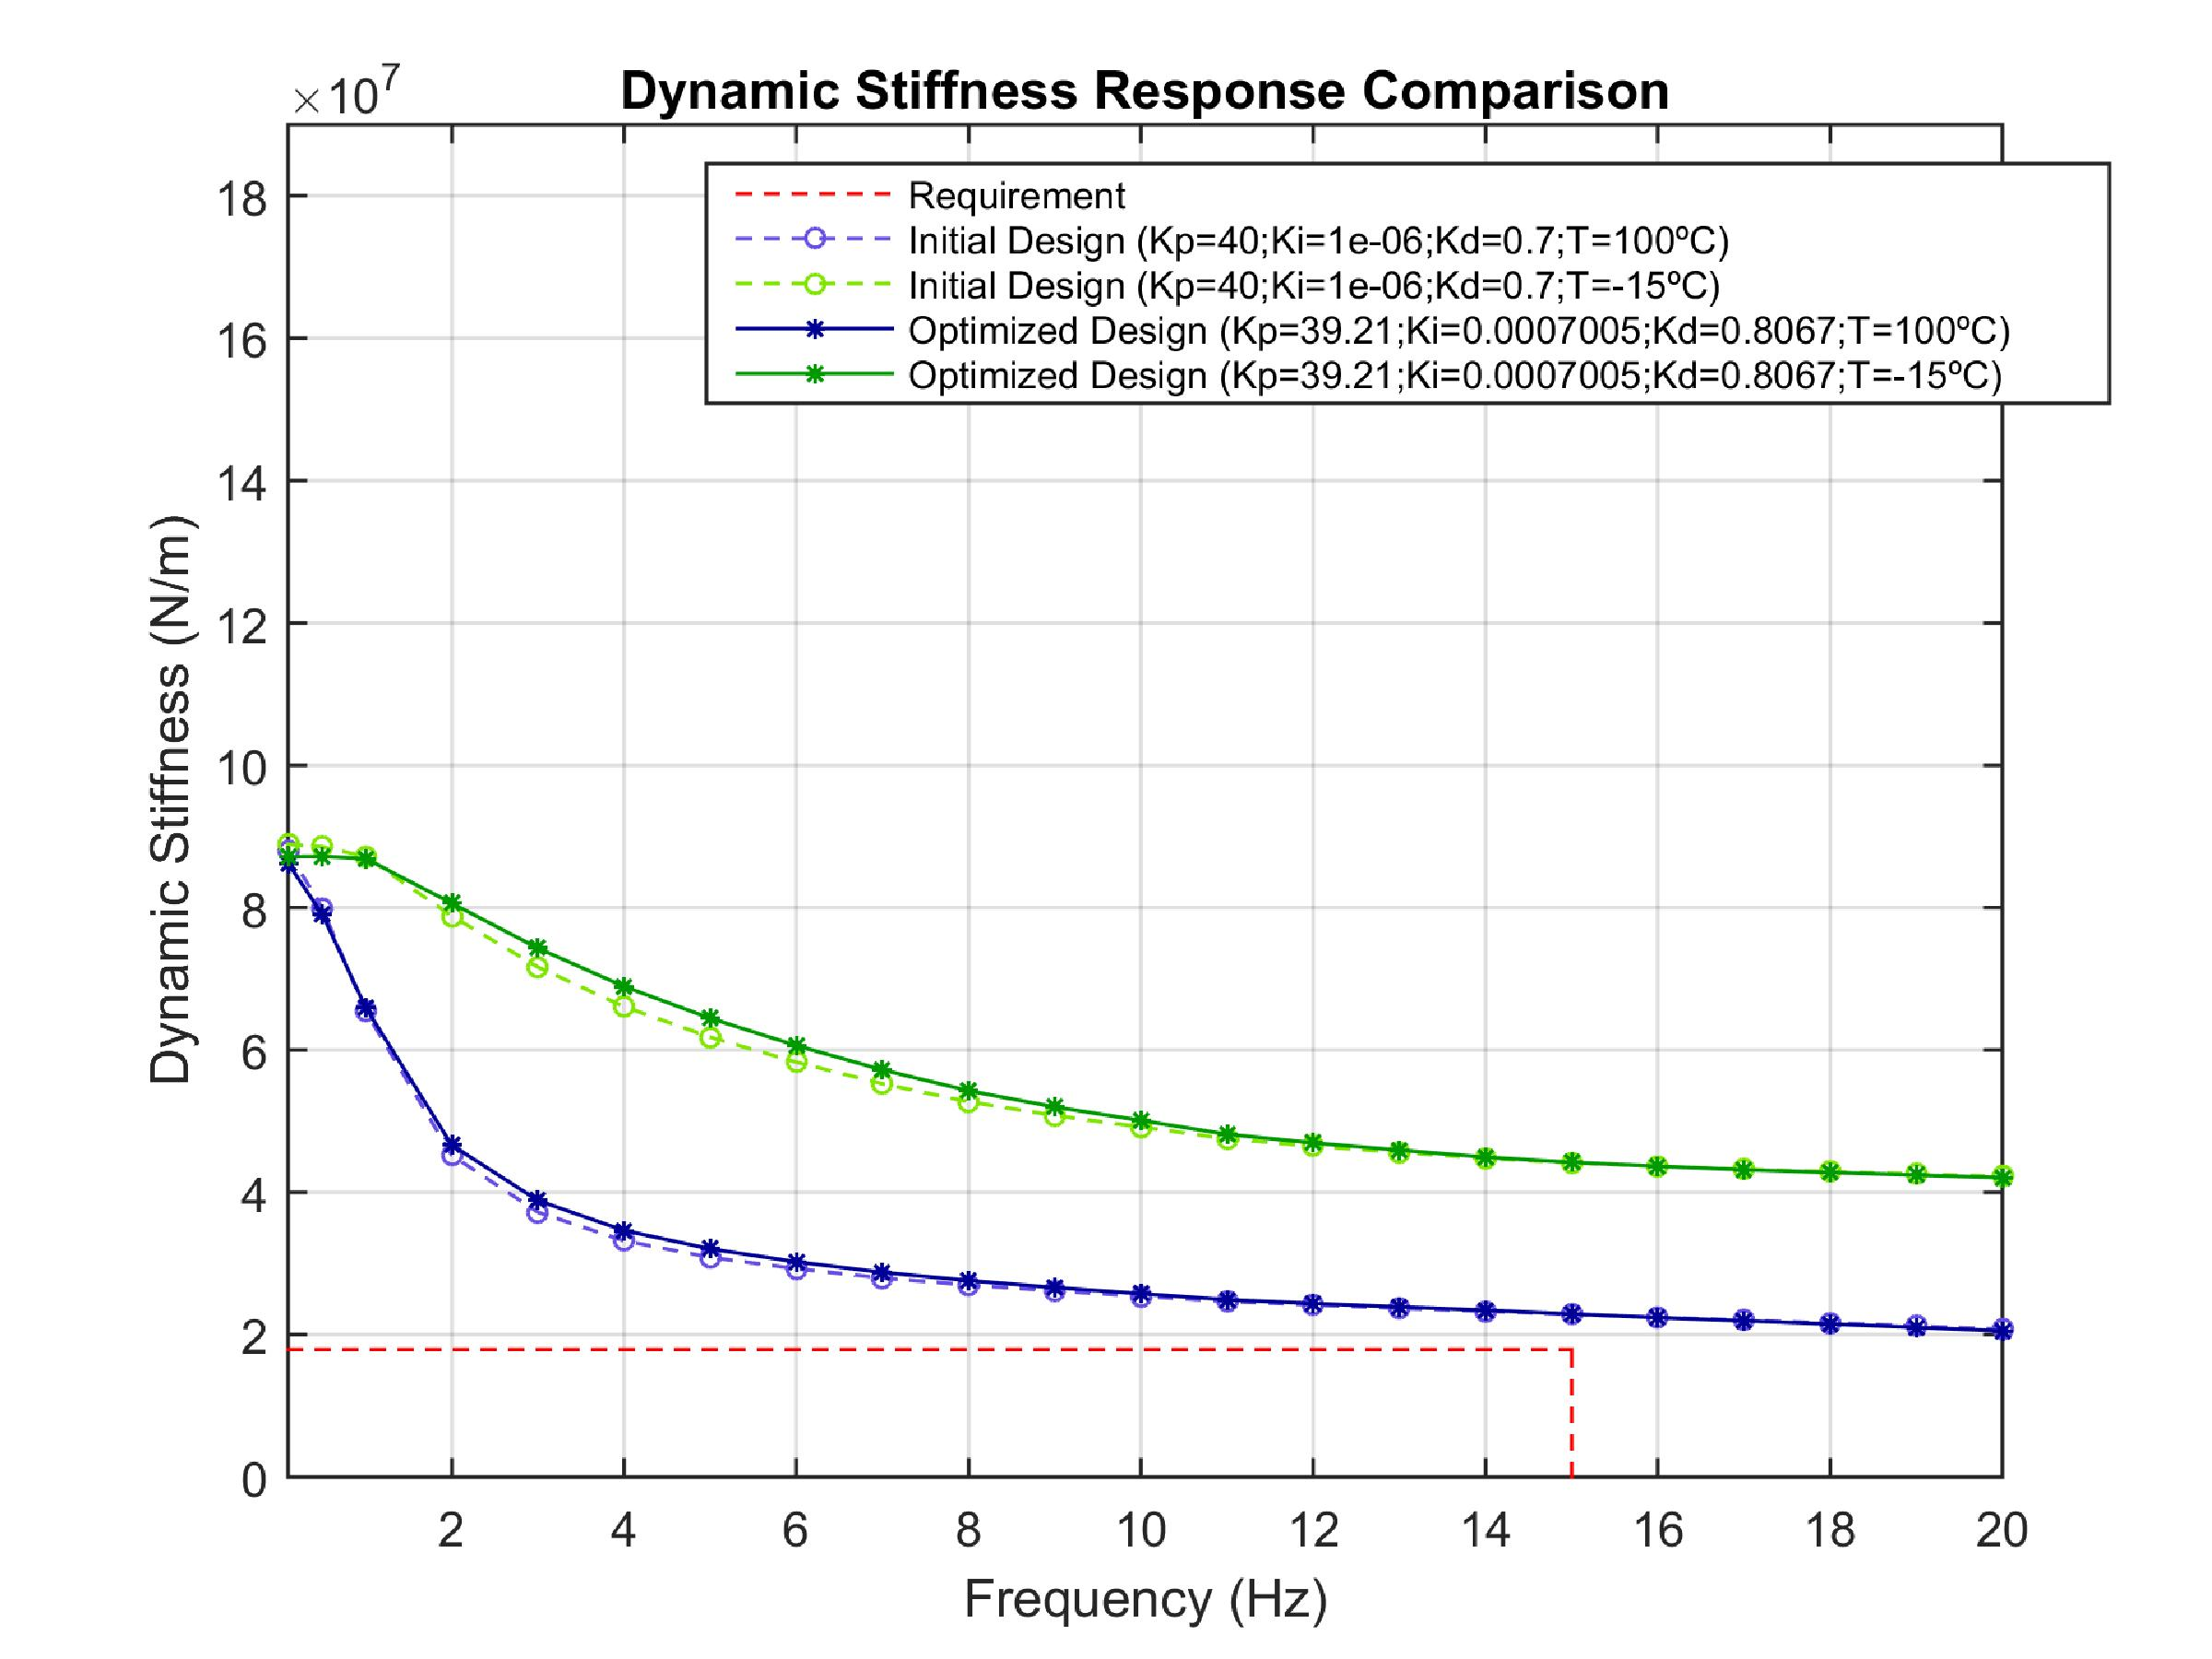
\includegraphics[width=0.9\textwidth]{Figuras/5.OptimizationResults/5-2-4-PID-DynamicStiffnessComparison.jpg}}
	\caption{Dynamic Stiffness Optimization Result for the PID Controller.}
	\label{fig:5_2_4_PID_DynStif}
\end{figure}

Table \ref{table:5_2_4_PID_CostFunctionTable} show the partial values of the cost function for each frequency evaluated by the dynamic stiffness test. The lower frequencies values are also larger than the higher frequency ones since stiffness is still greater in this range. 

\begin{table}[H]
	\captionof{table}{PID Controller Final Solution Cost Function for Each Evaluated Frequency}
	\label{table:5_2_4_PID_CostFunctionTable}
	\centering
	\resizebox{14cm}{!} {
		\begin{tabular}{|c|c|c|c|c|c|}
			\hline
			Frequency (Hz) & $J_i$ & Frequency (Hz) & $J_i$ & Frequency (Hz) & $J_i$ \\ \hline
			$0.1$ & $6.83e+07$ & $5$ & $1.42e+07$ & $11$ & $7.02e+06$ \\ \hline
			$0.5$ & $6.11e+07$ & $6$ & $1.23e+07$ & $12$ & $6.49e+06$ \\ \hline
			$1$ & $4.81e+07$ & $7$ & $1.08e+07$ & $13$ & $6e+06$ \\ \hline
			$2$ & $2.87e+07$ & $8$ & $9.7e+06$ & $14$ & $5.54e+06$ \\ \hline
			$3$ & $2.1e+07$ & $9$ & $8.72e+06$ & $15$ & $5.01e+06$ \\ \hline
			$4$ & $1.67e+07$ & $10$ & $7.86e+06$ & $0$ & $0$ \\ \hline
	\end{tabular}}
\end{table}

The time response comparison is presented in Figure \ref{fig:5_2_4_PID_TimeResp} and the performance requirements are shown in Table \ref{table:5_2_4_PID_PerfTable}. The settling time was increased by 10ms and the steady state error slightly increased. 

\begin{figure}[H]
	\centering
	\centerline{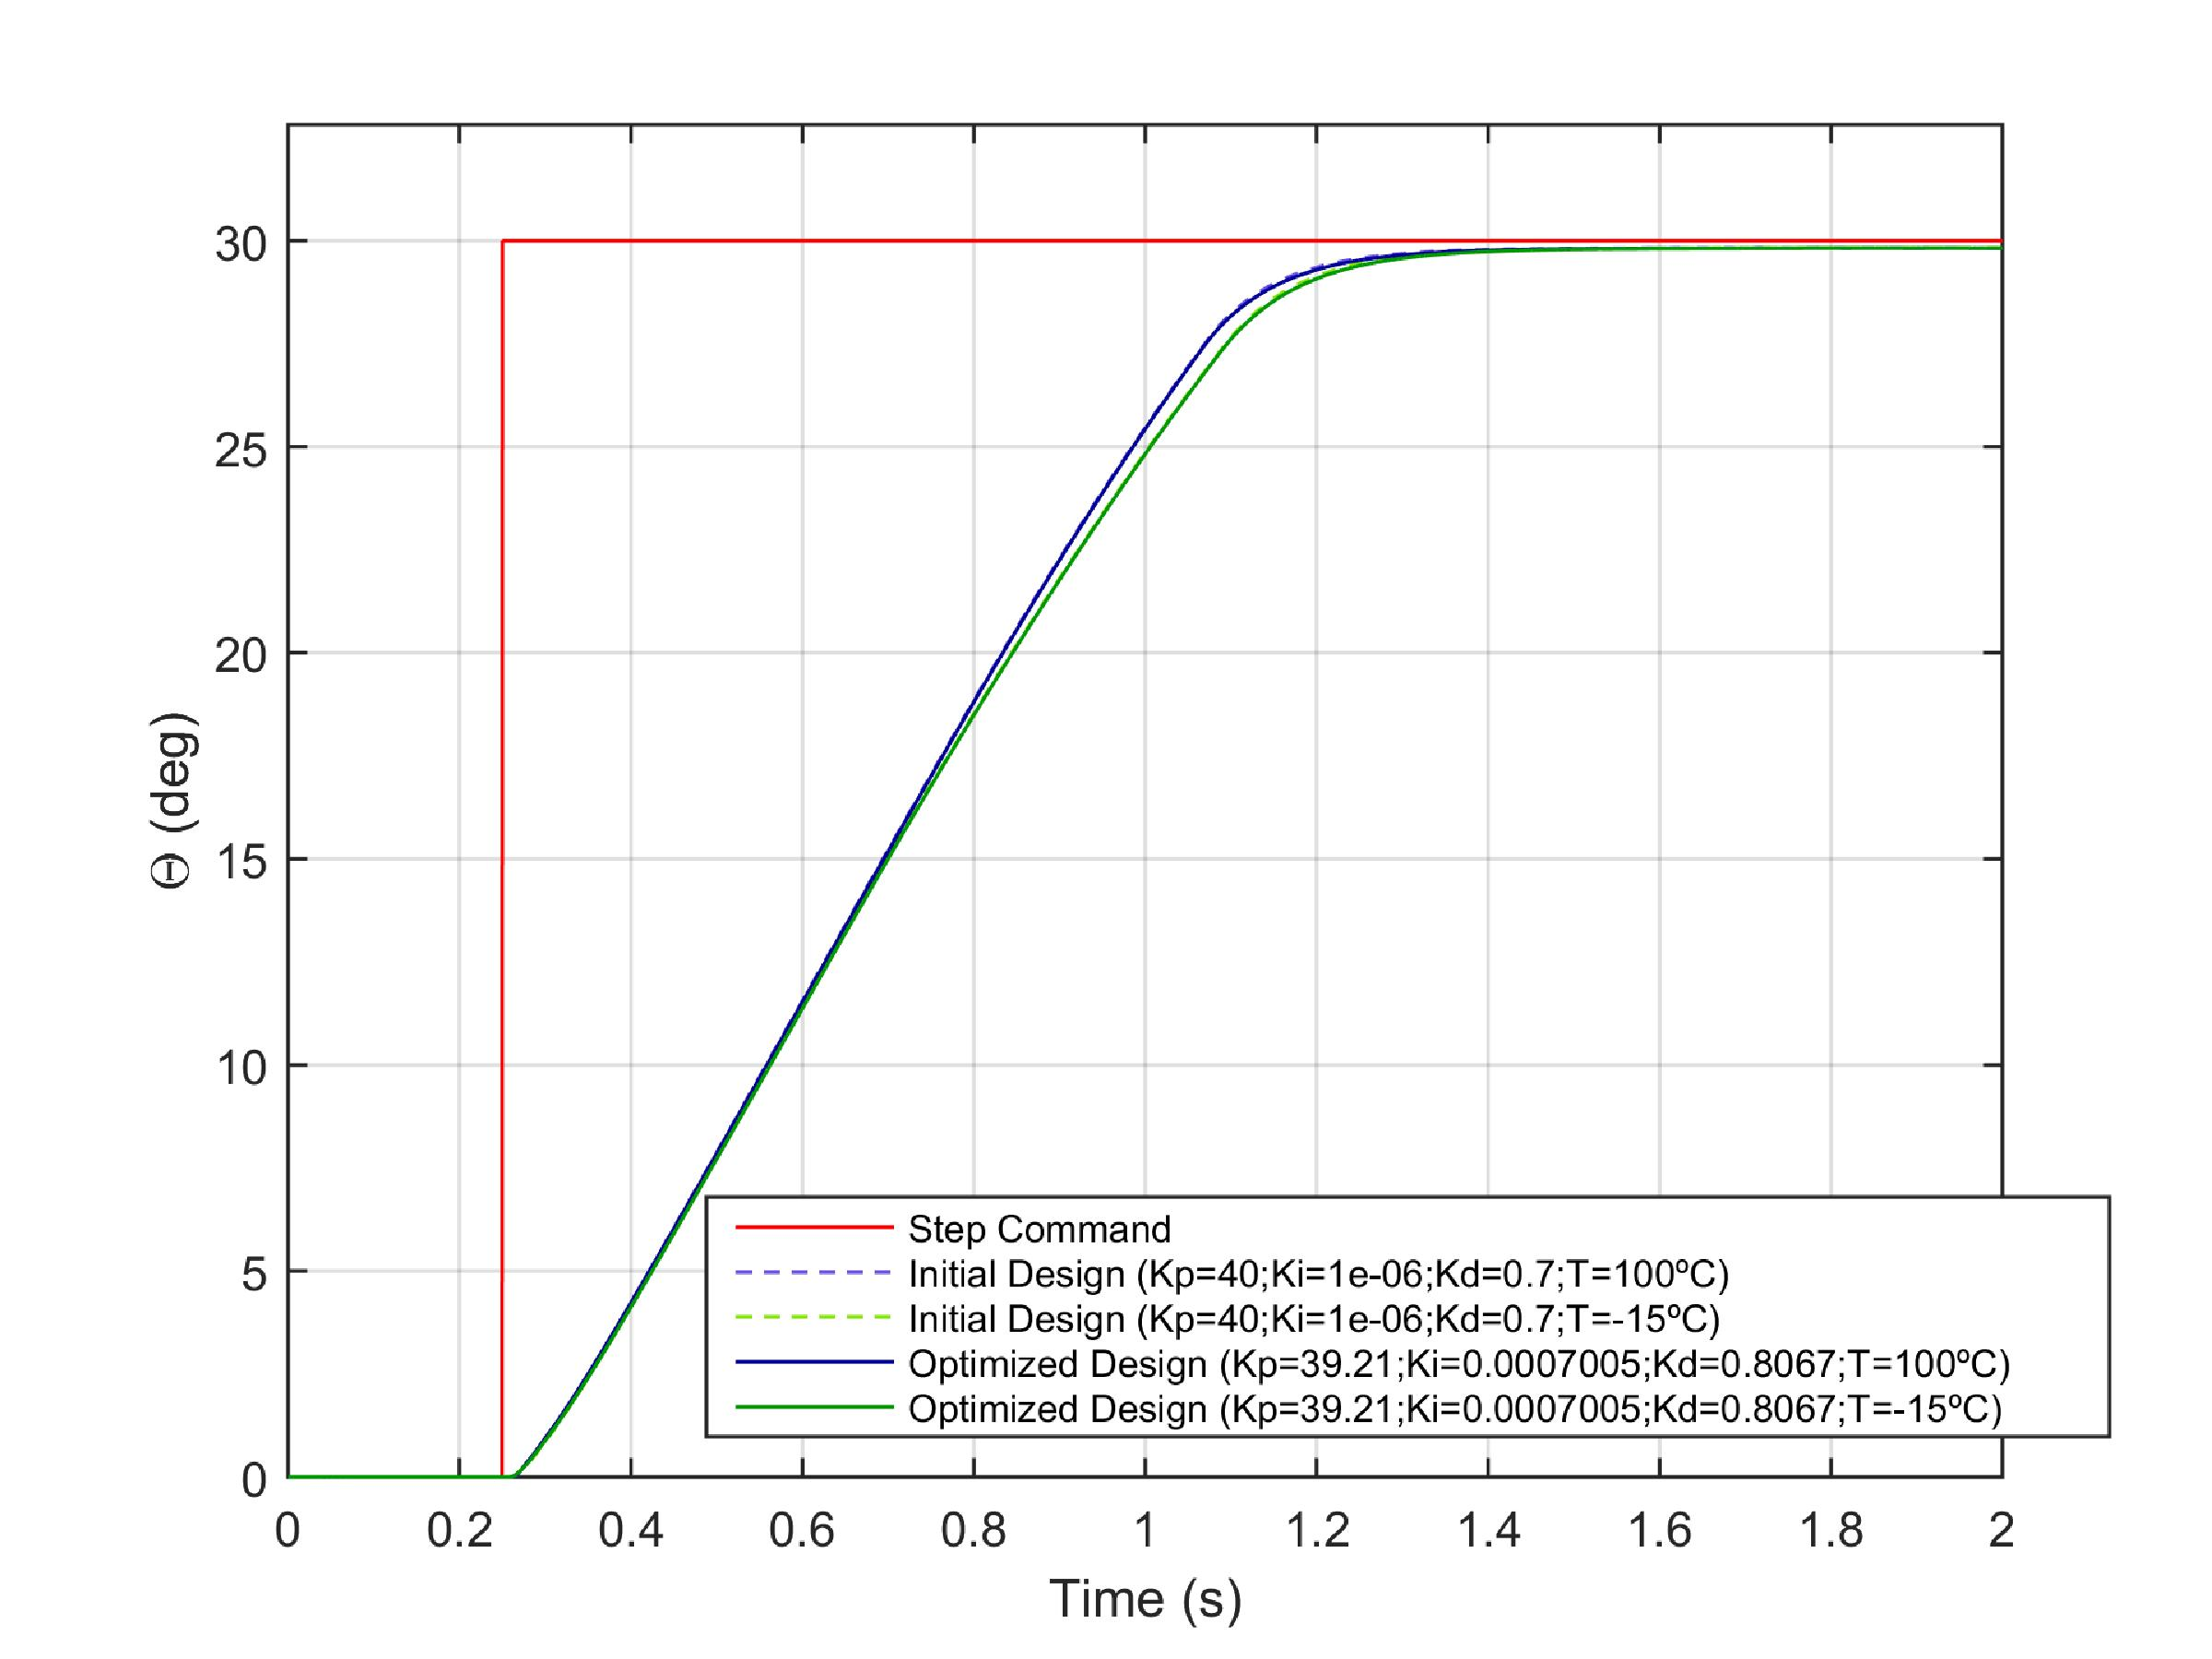
\includegraphics[width=0.9\textwidth]{Figuras/5.OptimizationResults/5-2-4-PID-TimeResponseComparison.jpg}}
	\caption{Time Response Optimization Result for the PID Controller.}
	\label{fig:5_2_4_PID_TimeResp}
\end{figure}

The closed-loop frequency response comparison is presented in Figure \ref{fig:5_2_4_PID_FreqResp} and the performance requirements are also shown in Table \ref{table:5_2_4_PID_PerfTable}. The closed-loop gain allowance was reduced to 12dB and the closed-loop phase allowance remained infinite. As for the PD controller, the performance parameters for the optimized PID did not reach or violate the requirements, suggesting that the solution is also a local minimum.

\begin{figure}[H]
	\centering
	\centerline{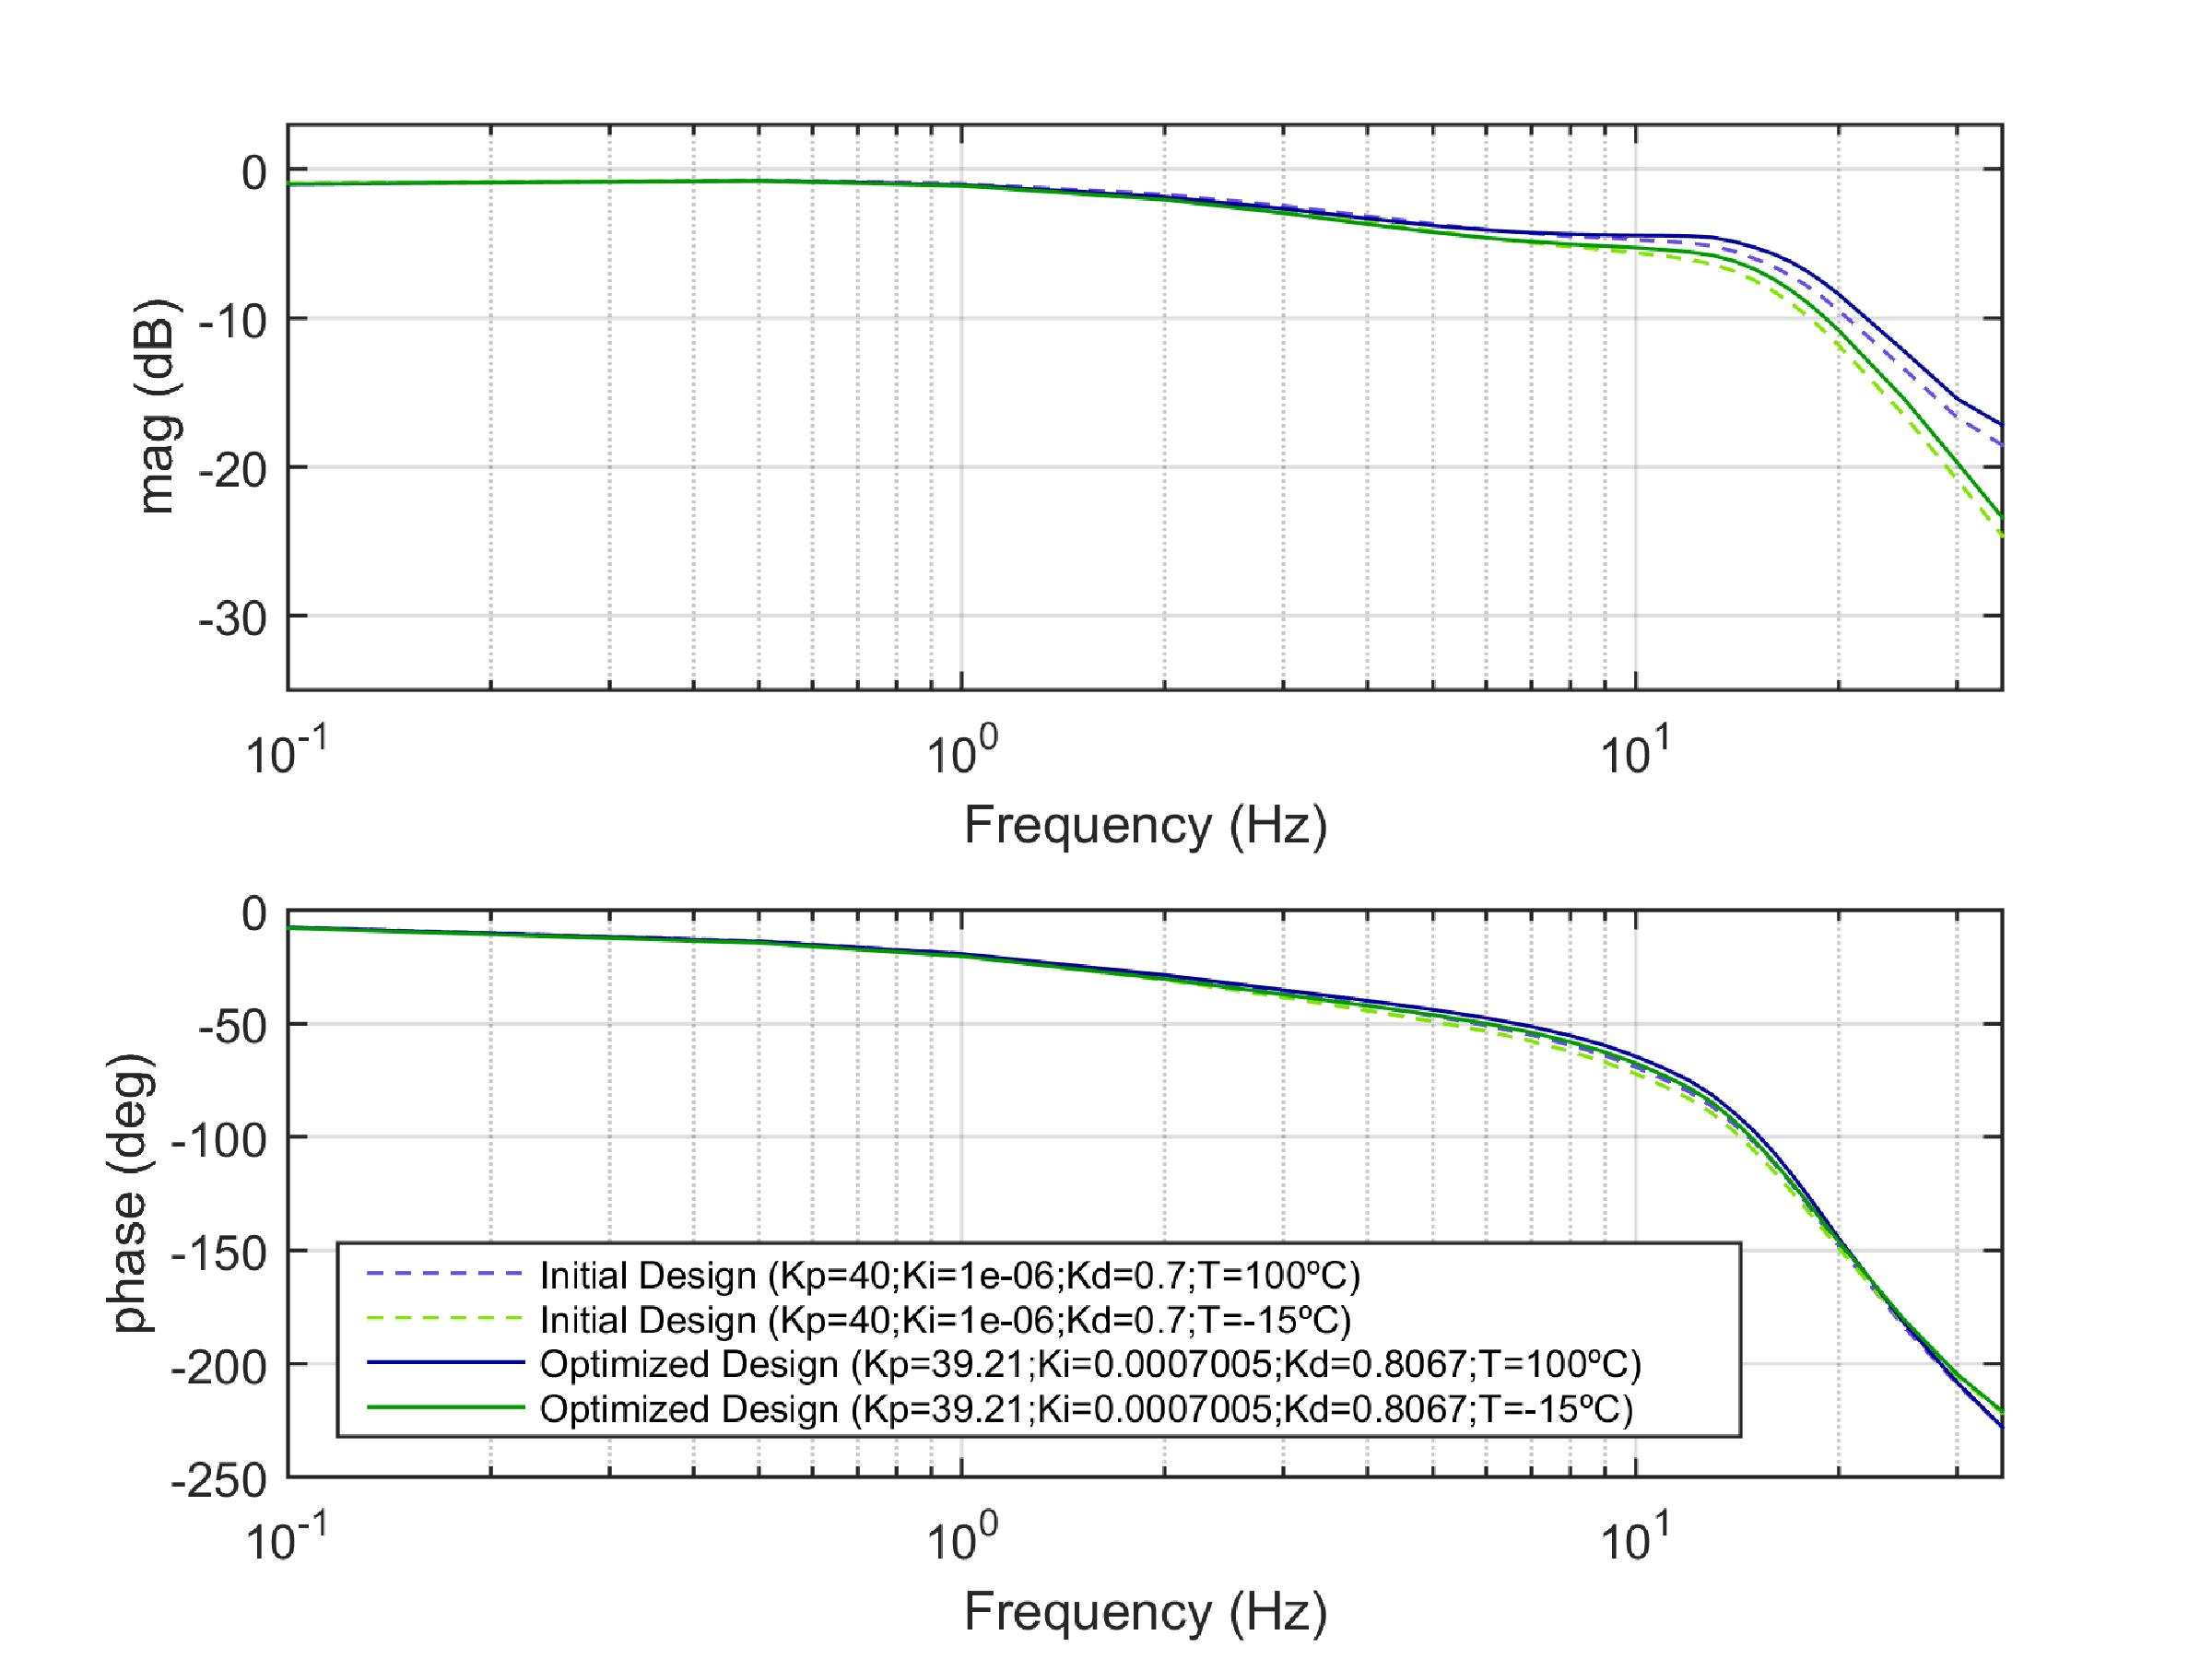
\includegraphics[width=0.9\textwidth]{Figuras/5.OptimizationResults/5-2-4-PID-FrequencyResponseComparison.jpg}}
	\caption{Frequency Response Baseline for the PID Controller.}
	\label{fig:5_2_4_PID_FreqResp}
\end{figure}

\begin{table}[H]
	\captionof{table}{Requirement Compliance for PID Controller}
	\label{table:5_2_4_PID_PerfTable}
	\centering
	\resizebox{14cm}{!} {
		\begin{tabular}{|l|c|c|c|c|}
			\hline
			Design Parameter & Requirement & Baseline & Optimized Controller & Difference (\%) \\ \hline
			Settling Time (ms) & $< 1100$ & $992$ & $1002$ & $1.0$ \\ \hline
			Steady State Error ($\%$) & $< 1$ & $0.27$ & $0.28$ & $3.7$ \\ \hline
			Overshoot ($\%$) & $< 10$ & $0$ & $0$ & $N/A$ \\ \hline
			Minimum Average Rate ($°$/s) & $> 32$ & $34.32$ & $34.28$ & $-0.1$ \\ \hline
			Maximum Average Rate ($°$/s) & $< 36$ & $34.32$ & $34.28$ & $-0.1$ \\ \hline
			Closed-Loop Gain Allowance (dB) & $> 10$ & $13$ & $12$ & $-7.7$ \\ \hline
			Closed-Loop Phase Allowance ($°$) & $> 45$ & $inf$ & $inf$ & $N/A$ \\ \hline
			Closed-Loop Maximum Peak (dB) & $< 0.5$ & $-0.74$ & $-0.77$ & $-4.1$ \\ \hline
			Closed-Loop Initial Magnitude(dB) & $None$ & $-0.99$ & $-1.01$ & $-2.0$ \\ \hline
			Closed-Loop Bandwidth (Hz) & $None$ & $5.83$ & $5.75$ & $-1.4$ \\ \hline
	\end{tabular}}
\end{table}

The results obtained with the frequency weighted cost function follow the same pattern observed previously: P and PI results are fairly similar as well as PD and PID results. In addition, optimization for all controllers yielded improvement in overall dynamic stiffness as expected. Also, it was possible to improve stiffness in higher frequencies, therefore, achieving the goal of the weighted cost function. Additionally, almost all optimizations were performed in less iterations and objective function executions, resulting in reduced execution times.

The results were aligned with the hypothesis that to increase dynamic stiffness in high frequencies a reduction in time domain performance would be required. P and PI controllers results show this clearly whereas PD and PID time performance were not affected substantially.

Other interesting observation is that P and PI controllers basically improved dynamic stiffness by having their proportional gain reduced until a constraint was violated. This happened because for these controllers only one design variable ($K_p$) effectively change dynamic stiffness, what naturally makes the optimization tend to one or the other bound of this gain. 

On the other hand, PD and PID controllers gains were fine tuned around the initial solution and probably converged to local minimums. In this case, \textit{fmincon} had two variables to use and many combinations of them to explore.

In summary, this section has shown that optimization with the frequency weighted cost function not only yielded controllers with better flutter suppression characteristics but also were executed faster than the optimizations with the previous cost function. 

\section{Optimization Constraints Sensitivity}

The optimization results are directly affected by the constraints imposed in the evaluated solutions. This naturally leads to the question: what would be the result if one or more constraints were slightly different? This section will present a constraint sensitivity analysis that aims to answer this question. The results obtained with the simple cost function will not be considered in this analysis as their results were not satisfactory.

\subsection{P and PI Controllers}

As discussed previously, the behavior of P and PI controllers optimization was very similar and therefore their sensitivity analysis is the same.

The optimization of these controllers was effectively performed by tuning the proportional gain which has a decreasing monotonic relationship with dynamic stiffness at 15Hz i.e. stiffness at this frequency tends to increase with proportional gain reduction. 

Therefore, the optimization reduced $K_p$ until a constraint was violated, in this case the settling time, as shown in Tables \ref{table:5_2_1_P_PerfTable} and \ref{table:5_2_2_PI_PerfTable}. If the settling time requirement was greater, $K_p$ would be smaller and the dynamic stiffness at 15Hz would be higher. In this case, closed-loop gain allowance would increase and closed-loop phase allowance would remain infinite hence, their requirements would not be violated. On the other hand, steady state error would increase and average rate would decrease and depending on how greater is the settling time this requirements could not be achieved.

The opposite would happen if the settling time requirement was smaller. In this case, $K_p$ would be greater, steady state error would be smaller and average rate would be higher. The closed-loop frequency response parameters would be jeopardized but would hardly violate their requirements.

For these controllers, the performance parameters did not reach the other constraints. Hence, any slight change of these requirements would not impact the obtained results.

The optimization with the weighted cost function was performed for the proportional controller with changes in the settling time constraint to confirm the expected results discussed in this section. Figure \ref{fig:5_3_1_P_DynStifTsComp} shows the behavior of the dynamic stiffness with a variation of $\pm10\%$ in the settling time requirement. 

As expected, the dynamic stiffness at 15 Hz increased when the settling time requirement was greater while the proportional gain decreased. Also, when the settling time requirement was reduced, the dynamic stiffness decreased and the proportional gain increased.

\begin{figure}[H]
	\centering
	\centerline{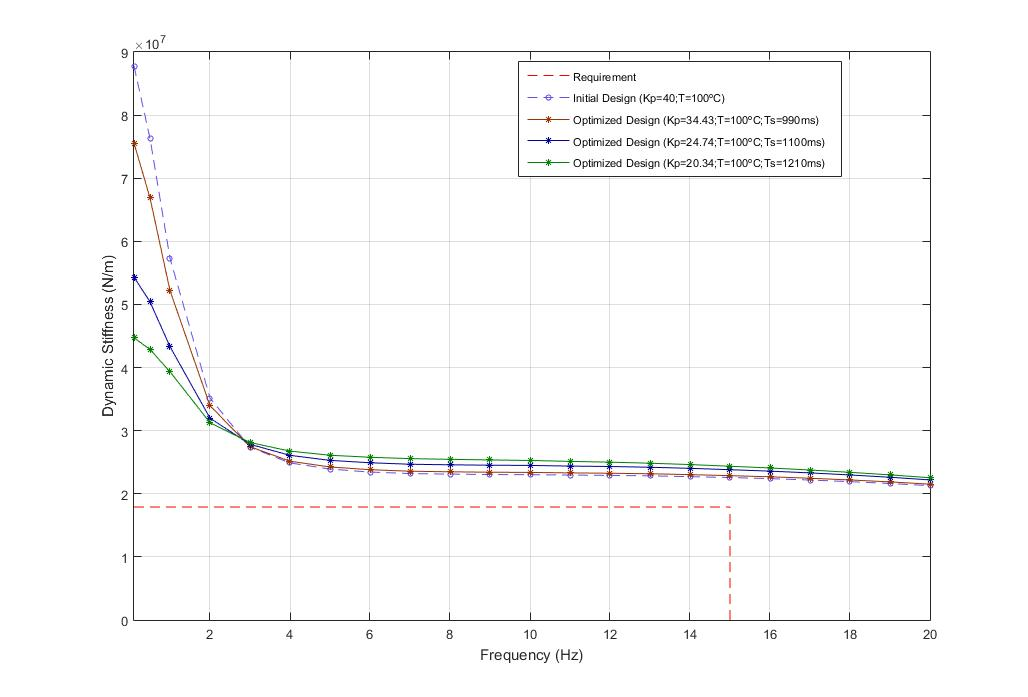
\includegraphics[width=0.9\textwidth]{Figuras/5.OptimizationResults/5-3-1-P-DynStiff-TsComp.jpg}}
	\caption{Optimized Dynamic Stiffness of Proportional Controller for Different Settling Time Requirements}
	\label{fig:5_3_1_P_DynStifTsComp}
\end{figure}

Table \ref{table:5_3_1_P_PerfTableComp} presents the behavior of the constraints in this analysis for each Optimized Controller (OC).

\begin{table}[H]
	\captionof{table}{Requirement Compliance of Proportional Controller for Different Settling Time Requirements}
	\label{table:5_3_1_P_PerfTableComp}
	\centering
	\resizebox{16cm}{!} {
		\begin{tabular}{|l|c|c|c|c|c|}
			\hline
			Design Parameter & Requirement & Baseline & OC (Ts-10\%) & OC (Ts=1100ms) & OC (Ts+10\%) \\ \hline
			Settling Time (ms) 		& $<990/<1100/<1210$ 	& $959$   & $990$   & $1101$  & $1211$  \\ \hline
			Steady State Error ($\%$) 			& $< 1$ 	& $0.27$  & $0.31$  & $0.43$  & $0.53$  \\ \hline
			Overshoot ($\%$) 					& $< 10$ 	& $0$     & $0$     & $0$     & $0$     \\ \hline
			Minimum Average Rate ($°$/s) 		& $> 32$ 	& $34.45$ & $34.36$ & $34.09$ & $33.78$ \\ \hline
			Maximum Average Rate ($°$/s) 		& $< 36$ 	& $34.45$ & $34.36$ & $34.09$ & $33.78$ \\ \hline
			Closed-Loop Gain Allowance (dB) 	& $> 10$ 	& $20.35$ & $22.56$ & $28.21$ & $32.70$ \\ \hline
			Closed-Loop Phase Allowance ($°$) 	& $> 45$ 	& $inf$   & $inf$   & $inf$   & $inf$   \\ \hline
			Closed-Loop Maximum Peak (dB) 		& $< 0.5$ 	& $-0.65$ & $-0.82$ & $-1.38$ & $-1.90$ \\ \hline
			Closed-Loop Initial Magnitude(dB)   & $None$ 	& $-1.0$  & $-1.2$  & $-1.9$  & $-2.5$  \\ \hline
			Closed-Loop Bandwidth (Hz) 			& $None$ 	& $6.3$   & $5.1$   & $3.3$   & $2.5$   \\ \hline
	\end{tabular}}
\end{table}

As expected, the response is faster and with less error when the settling time requirement is reduced and vice-versa. Additionally, the closed-loop gain allowance increased even more with a greater settling time requirement while the bandwidth was fairly reduced.

\subsection{PD and PID Controllers}

The behavior of PD and PID controllers optimization was also very similar. In this case, two variables, $K_p$ and $K_d$, were effectively used to achieve greater dynamic stiffness. Thus, the relationship between the design variables and the objective function was more complex and no longer monotonic.

This explains why no constraint was violated or reached by the performance parameters. As shown in Tables \ref{table:5_2_3_PD_PerfTable} and \ref{table:5_2_4_PID_PerfTable}, a slight change in requirements ($\pm5\%$) would not make the obtained solutions infeasible. Even a greater change ($\pm15\%$) would not invalidate the solutions unless it is applied to the settling time requirement. However, in this case not even the initial solution would be feasible therefore the optimization would most likely decrease dynamic stiffness at the infinite frequency.
%
%\section{Infinite Frequency Weight Sensitivity}
%
%Another interesting analysis is to understand how sensitive is the objective function and if it can be changed to improve the obtained results. This investigation was performed for the PD controller, since its optimization did not reach any constraints and its results were similar to the PID. 
%
%An increase in the relative importance of the infinite frequency might influence the objective function to change its local minima in a way that rewards more dynamic stiffness increase at that frequency. 
%
%The optimization program was executed for three different values of parameter $\gamma_{15Hz}$: 4, 5 and 6. Figure \ref{fig:5_4_P_DynStifGammaComp} shows the dynamic stiffness of the optimized controllers obtained with each $\gamma_{15Hz}$.
%
%\begin{figure}[H]
%	\centering
%	\centerline{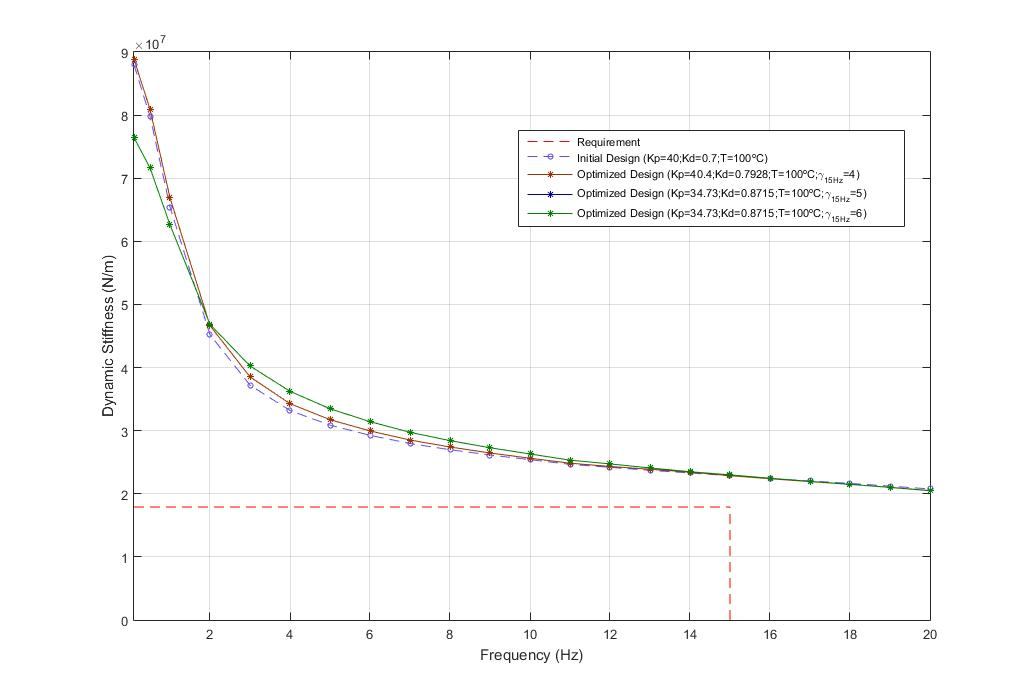
\includegraphics[width=0.9\textwidth]{Figuras/5.OptimizationResults/5-4-PD-DynStiff-WeigComp.jpg}}
%	\caption{Optimized Dynamic Stiffness of PD Controller for Different Infinite Frequency Weights}
%	\label{fig:5_4_P_DynStifGammaComp}
%\end{figure}
%
%The curve for a $\gamma_{15Hz}$ of 4 has a different behavior to what was previously observed. In this case, dynamics stiffness increased slightly in all frequencies up to 15 Hz and decreased otherwise. Despite this, the stiffness increase at 15 hz was fairly small as per Table \ref{table:5_4_DynStiffComp}.
%
%The curve for $\gamma_{15Hz}$ of 5 and 6 were the same, showing that the limitation of dynamic stiffness improvement by the controller.
%
%\begin{table}[H]
%	\captionof{table}{Dynamic Stiffness of PD Controller for Different Infinite Frequency Weights}
%	\label{table:5_4_DynStiffComp}
%	\centering
%	\resizebox{12cm}{!} {
%		\begin{tabular}{|l|c|c|}
%			\hline
%			Design 							& 15 Hz Dynamic Stiffness $(10^{7} N/m)$ & Difference (\%)	\\ \hline
%			Baseline						& $2.2853$ & $N/A$		\\ \hline
%			Optimized ($\gamma_{15Hz}=4$) 	& $2.2875$ & $0.1$		\\ \hline
%			Optimized ($\gamma_{15Hz}=5$) 	& $2.2918$ & $0.3$		\\ \hline
%			Optimized ($\gamma_{15Hz}=6$)	& $2.2994$ & $0.6$		\\ \hline
%	\end{tabular}}
%\end{table}
%
%\begin{table}[H]
%	\captionof{table}{Requirement Compliance of PD Controller for Different Infinite Frequency Weights}
%	\label{table:5_4_P_PerfTableComp}
%	\centering
%	\resizebox{16cm}{!} {
%		\begin{tabular}{|l|c|c|c|c|c|}
%			\hline
%			Design Parameter & Requirement & Baseline & OC ($\gamma_{15Hz}=4$) & OC ($\gamma_{15Hz}=5$) & OC ($\gamma_{15Hz}=6$) \\ \hline
%			Settling Time (ms) 					& $<1100$ 	& $992$   & $994$   & $1006$  & $1041$  \\ \hline
%			Steady State Error ($\%$) 			& $< 1$ 	& $0.27$  & $0.27$  & $0.28$  & $0.31$  \\ \hline
%			Overshoot ($\%$) 					& $< 10$ 	& $0$     & $0$     & $0$     & $0$     \\ \hline
%			Minimum Average Rate ($°$/s) 		& $> 32$ 	& $34.32$ & $34.31$ & $34.27$ & $34.20$ \\ \hline
%			Maximum Average Rate ($°$/s) 		& $< 36$ 	& $34.32$ & $34.31$ & $34.27$ & $34.20$ \\ \hline
%			Closed-Loop Gain Allowance (dB) 	& $> 10$ 	& $13.0$  & $12.0$  & $12.0$  & $12.0$  \\ \hline
%			Closed-Loop Phase Allowance ($°$) 	& $> 45$ 	& $inf$   & $inf$   & $inf$   & $inf$   \\ \hline
%			Closed-Loop Maximum Peak (dB) 		& $< 0.5$ 	& $-0.74$ & $-0.74$ & $-0.79$ & $-0.95$ \\ \hline
%			Closed-Loop Initial Magnitude(dB)   & $None$ 	& $-0.99$ & $-0.98$ & $-1.03$ & $-1.19$ \\ \hline
%			Closed-Loop Bandwidth (Hz) 			& $None$ 	& $5.8$   & $6.2$   & $5.6$   & $4.5$   \\ \hline
%	\end{tabular}}
%\end{table}
%
%
%
%
%
%
%
